\documentclass[twoside,11pt]{Latex/Classes/PhDthesisPSnPDF}
%         PUEDEN INCLUIR EN ESTE ESPACIO LOS PAQUETES EXTRA, O BIEN, EN EL ARCHIVO "PhDthesisPSnPDF.cls" EN "./Latex/Classes/"

\usepackage{blindtext}                        % Para insertar texto dummy, de 
%--------------------Cambiar captio de las subfiguras -------------------
\renewcommand*{\thesubfigure}{\alph{subfigure})}   %Cambia caption y también el \ref{   }  

	\newcommand{\beqhalf}{\noindent \begin{minipage}[c]{.5\linewidth} \begin{equation}}
	\newcommand{\eeqhalf}{\end{equation} \end{minipage} }
	\newcommand{\eqhalf}[1]{\beqhalf #1 \eeqhalf}	


\usepackage{animate}  %pARA EL GIF



%\makeatletter
%\newenvironment{taggedsubequations}[1]
% {%
%  % \end{subequations} will advance `equation`
%  \addtocounter{equation}{-1}%
%  \begin{subequations}%
%  % set the current label
%  \def\@currentlabel{#1 \emph{bis}}%
%  % redefine \theequation
%  \renewcommand{\theequation}{#1\alph{equation} \emph{bis}}%
% }
% {\end{subequations}}
%\makeatother %not \makeatletter

\makeatletter
\newenvironment{taggedsubequations}[1]
 {%
  % \end{subequations} will advance `equation`
  \addtocounter{equation}{-1}%
  \begin{subequations}%
  % set the current label
  \def\@currentlabel{#1}%
  % redefine \theequation
  \renewcommand{\theequation}{#1\alph{equation}}%
 }
 {\end{subequations}}
\makeatother %not \makeatletter




%%% Local Variables:
%%% mode: latex
%%% TeX-master: "~/Documents/LaTeX/CUEDThesisPSnPDF/thesis"
%%% End:
           % Archivo con funciones útiles

\usepackage{setspace}

%%-------------------------------------------------------------------------------
%                                   DATOS                                      |
%-------------------------------------------------------------------------------
\title{Título de la tesis}
\author{Jonathan Alexis Urrutia Anguiano}        
\degree{Licenciatura en Física}               % Carrera
\director{Dr. Alejandro Reyes Coronado}       % Asesor
\degreedate{YYYY}                           	% Año de la fecha del examen
\lugar{México, Cd. de México}          		% Lugar
\portadatrue                                	% Portada en COLOR


\keywords{tesis,autor,tutor,etc}            % Palablas clave para los metadatos del PDF
\subject{tema_1,tema_2}                     % Tema para metadatos del PDF  
%-------------------------------------------------------------------------------
%                                   PORTADA                                    |
%-------------------------------------------------------------------------------
\begin{document}

\maketitle									
%-------------------------------------------------------------------------------
%                                   Prologo                                    |
%-------------------------------------------------------------------------------
\frontmatter

%\begin{dedication}
Frase motivacional preferida
Yo.
\end{dedication}
       
%% !TeX root = ../tesis.tex
\begin{acknowledgements}
\addcontentsline{toc}{chapter}{\protect\numberline{}Agradecimientos}
\small
\vspace*{2.5em}

En estas líneas agradezco a quienes me brindaron apoyo y me guiaron durante mis estudios profesionales en la Universidad Nacional Autónoma de México (UNAM). Primeramente, en el ámbito académico, agradezco al Dr. Alejandro Reyes Coronado por sus consejos a lo largo de varios años de trabajo junto a él; a la Dra. Citlali Sánchez Aké por permitirme acercarme al trabajo experimental en su laboratorio; al Dr. Rubén Gerardo Barrera y Pérez no sólo por sus enseñanzas en la física, sino por mostrarme que la vida hay que disfrutarla;  al Dr. Guiseppe Pirruccio por sus valiosos comentarios y críticas al trabajo; y a la Dra. Celia Sánchez Pérez por todo su apoyo en este proceso. Asimismo, agradezco al proyecto  DGAPA-UNAM PAPIIT IN114919 por el apoyo económico que me otorgó a lo largo de un año para desarrollar mi trabajo de tesis de licenciatura y al programa de movilidad estudiantil de la Dirección General de Cooperación e Internacionalización por corroborar que la formación que me dio la UNAM compite con la de cualquier lado del mundo.

También quiero reconocer el esfuerzo de mi familia: a mi mamá, quien, entre muchas otras cosas, me enseñó que lo que uno hace por los demás no es una molestia sino una muestra de cariño; a mi papá, por desarrollar un interés en lo que me apasiona y conocerme a través de ello; a mis hermanas, Abby y Dianis, por aconsejarme desde la experiencia y el entendimiento en la que fue una nueva etapa; y a Mamá Bola y a Tío Beto, por todo lo que fueron para mí.

Igualmente, le doy las gracias a quienes me siguen acompañando desde hace varios ayeres: a Ximena LP, David de Aragón, Adrián AJ, Bryan ChH, Oscar OR y Claudio ER por amistades eternas basadas en discutir, en escuchar, en descubrir, en reconocer, en confiar y en apoyar, respectivamente, y que con el paso del tiempo sólo ganan fortaleza y significado para mí; y a Karla GB, por forjar conmigo una relación que, pese a nuestro reniegue por el otro, ha sido de las más valiosas.

Finalmente, les ofrezco (en orden cronológico) mis más sinceras palabras de gratitud por una camaradería siempre creciente: a Leo GP, por brindarme una  amistad que me costó el último bocado de chilaquiles, el cual cedería de nuevo; a Martín GT, por cada historia contada en 4.49 s; a Clau GR, por las intermitentes, pero siempre gratificantes, pláticas rondando por la ciudad; a AJ Polanco, por tus habilidades culinarias y por encarnar la fidelidad con los amigos; a EA Conde, por su sinceridad perpetua y clases de baile; a Jorge BD, por compartir conmigo \emph{el juego} de la ayudantía, la tesis y los propes; a Diana PV, por el asilo en su cubo y la confianza que nos dimos; a Mariana dBF, por enseñarme nuevas formas de aprender y el mensaje de Moby Dick: ser tú mismo; a Juan José BM, por ser las Prispas en medio de las Pringles (en varios sentidos); \textit{Karen LM, für die schöne Piñata und die unerwartete Freundschaft}; \textit{den faulen Veronika Z, Darko C und C Ying, die meine Familie waren und mit denen ich nur Abenteuer erlebte}; al gran JC, por las clases de mecánica y termo, pero también por mostrar determinación en lo que se quiere; y (nuevamente) a Clau GR por permitirme conocernos de nuevo, aprender del otro y crecer juntos.













%\blindtext % Dummy text
\end{acknowledgements}




    
%\include{0-2-Declaracion/1-Declaracion}           
%
% Thesis Abstract -----------------------------------------------------

%\begin{abstractslong}    %uncommenting this line, gives a different abstract heading
\begin{abstracts}        %this creates the heading for the abstract page
\addcontentsline{toc}{chapter}{\protect\numberline{}Resumen}
\vspace{-1em}

Los biosensores plasmónicos comerciales emplean plasmones-polaritones de superfice (SPPs) excitados en una película continua de oro. Se han propuesto arreglos nanoestructurados tanto periódicos como desordenados para mejorar la sensibilidad de los sensores comerciales empleando las resonancias plasmónicas de red de superficie (PSLRs) y  las resonancias de plasmón de superficie localizadas (LSPRs),  respectivamente, sin embargo, su fabricación es costosa y tardada. Con el modelo de esparcimiento coherente (CSM) se analiza de forma teórica la reflectancia de una monocapa desordenada de nanopartículas (NPs) esféricas de oro y de plata y se evalúa su uso como sensor. El CSM predice un supuesto modo plasmónico colectivo, excitado en incidencia interna, que puede sintonizarse al elegir el radio $a$ de las NPs de la monocapa y su fracción de llenado $\Theta$. Los resultados con el CSM muestran que una monocapa desordenada de NPs de oro con radio $a=30$ nm y $\Theta=0.125$ y una de NPs de plata con $a=40$ nm y $\Theta=0.1$ pueden emplearse para el biosensado. La comparación del supuesto modo colectivo con la PSLR y la LSPR muestra sensibilidades comparables entre las tres resonancias para ángulos de incidencia cercanos al ángulo crítico. La comparación del supuesto modo plasmónico colectivo con el SPP muestra longitudes de penetración comparables a pesar de que el SPP cuenta con una sensibilidad y una figura de mérito de bulto mayores.

\vspace*{1cm}\textit{
Commercial plasmonic biosensors use surface plasmon-polaritons (SPPs) excited on a continuous gold film. Periodic and disordered nanostructured arrays have been proposed to improve the sensitivity of commercial sensors by employing Plasmonic Surface Lattice Resonances (PSLRs) and Localized Surface Plasmon Resonances (LSPRs), however their production time is long and their cost is expensive.  By using the coherent spreading model (CSM) the reflectance of a monolayer of spherical gold and silver nanoparticles (NPs) randomly arranged is theoretically analyzed and its use as a sensor is evaluated. The CSM predicts a possible collective plasmonic mode, excited in internal incidence, which can be tuned by choosing the radius $a$ of the NPs on the monolayer and its cover fraccion $\Theta$. The results with the CSM show that a monolayer of gold NPs with radius $ a = 30 $ nm and $ \Theta = 0.125 $, as well as one of silver NPs with $ a = 40 $ nm and $ \Theta = 0.1 $  can be used for biosensing. The comparison of the possible collective plasmonic mode against the PSLR and the LSPR shows comparable sensitivities between the three resonances for angles of incidence close to the critical angle. The comparison of the probable collective plasmonic mode with the SPP shows comparable penetration lengths even though the SPP has both a greater sensitivity and a greater figure of merit.}



\end{abstracts}
%\end{abstractlongs}


% ----------------------------------------------------------------------                  

%-------------------------------------------------------------------------------
%                                   Índices                                    |
%-------------------------------------------------------------------------------
%Esta sección genera el índice
\setcounter{secnumdepth}{3} % organisational level that receives a numbers
\setcounter{tocdepth}{3}    % print table of contents for level 3

\def\baselinestretch{1} 

\tableofcontents            % Genera el índice 

%: ----------------------- list of figures/tables ------------------------
%\listoffigures              % Genera el ínidce de figuras, comentar línea si no se usa
%\listoftables               % Genera índice de tablas, comentar línea si no se usa


%-------------------------------------------------------------------------------
%                                   Contents                                   |
%-------------------------------------------------------------------------------
% the main text starts here with the introduction, 1st chapter,...
\mainmatter

\def\baselinestretch{1}                   % Interlineado

\chapter*{Introducción}
\addcontentsline{toc}{chapter}{\protect\numberline{}Introducción}
\label{chapter:Motivacion}

%Presentación
%Objetivo

%Motivación
Las propiedades f\'isicas de los materiales dependen en general del tamaño del sistema \cite{boverhof2015comparative}, por ejemplo, a escala nanom\'etrica ---de $1$ a $100$ nm \cite{boverhof2015comparative}---, la respuesta electromagn\'etica (EM) de bulto de los metales es menos relevante que los efectos de superficie \cite{zhao2008methods}.  La \emph{nanoplasm\'onica} estudia la respuesta EM a esta escala y el inter\'es en su estudio se ha renovado debido a las posibles aplicaciones que emplean las resonancias plasm\'onicas de superficie (Surface Plasmon Resonances, SPRs).  Áreas como la espectroscop\'ia \cite{novotny2006principles}, el sensado \cite{jain2008noble}, la litograf\'ia \cite{stockman2011nanoplasmonics}, la biolog\'ia y  medicina \cite{jain2008noble}, son ejemplos del creciente interés en la nanoplasmónica. 

Otro ejemplo donde la nanoplasmónica ha impactado es en los \textit{biosensores} \cite{estevez2014trends,mun2015nanobiosensors}, definidos como ``dispositivos [$\ldots$] basados en elementos de reconocimiento biológico conectados a un transductor de señal, que relaciona la concentración de [uno o varios analítos] a una señal medible'' \cite{mun2015nanobiosensors}. Los biosensores se clasifican según el método de reconocimiento del analito, o bien, del transductor empleado \cite{mun2015nanobiosensors}. Dentro de los biosensores que ya se comercializan, los ópticos se caracterizan por su estabilidad, por sus mediciones sin marcadores, y por la  posibilidad de miniaturización y de multiplexeo \cite{estevez2014trends}, sobre todo los que se basan en nanoestructuras plasmónicas.

Los plasmones son oscilaciones colectivas de los electrones en un material metálico,  resultado del  acoplamiento con la radiaci\'on EM a las frecuencias en las que ocurren las SPRs \cite{stockman2011nanoplasmonics}.  Los plasmones pueden excitarse dentro de un metal (plasmones de volumen) o  sobre la superficie de alguna estructura metálica (plasmones de superficie) \cite{maier2007plasmonics}, en cuyo caso, los plasmones pueden ser de dos tipos: propagantes y localizados.  Cuando los plasmones se propagan a lo largo de una interfaz plana entre un medio diel\'ectrico y uno met\'alico se denomina  \emph{plasm\'on-polarit\'on de superficie} (Surface Plasmon Polariton, SPP) \cite{maier2007plasmonics}.  Si el plasmón, en cambio, se encuentra en la superficie de una partícula  met\'alica, de tamaño finito, se le conoce como \emph{resonancia de plasm\'on de superficie localizado} (Localized Surface Plasmon Resonance, LSPR) \cite{maier2007plasmonics}.

Los biosensores ópticos emplean las SPRs por la respuesta que tienen ante cambios del índice de refracción de la matriz \cite{kabashin2009plasmonic}, que es el medio que rodea la estructura metálica.  Los sensores comerciales se caracterizan por el uso de SPPs \cite{estevez2014trends} en una configuración de reflexión total atenuada (Attenuated Total Reflection, ATR), en donde el índice de refracción del medio donde incide la luz que ilumina a la estructura metálica es mayor al de la matriz (ver Fig.  \ref{fig:ATR1}).  Las mediciones de reflectancia, en un sistema en configuración ATR, presentan mínimos para determinadas combinaciones de  ángulos de incidencia $\theta_i$ y longitud de onda $\lambda$  \cite{danilov2018ultra}.  Los sensores basados en las LSPRs se han propuesto como mejora sobre los sensores comerciales \cite{estevez2014trends}, ya que estos son al menos un orden de magnitud más sensibles a cambios de índice de refracción de la matriz  que los sensores basados en SPPs \cite{jain2008noble,kabashin2009plasmonic}. \\

	\begin{figure}[h!]\centering
	\begin{subfigure}{.05\textwidth}\vspace{-3.5cm}\caption{}\label{sfig:Pols}\end{subfigure}
	\begin{subfigure}{.43\textwidth} 
		\includegraphics[scale=.225]{0-4-Introduccion/figs/SPP-3D.png}
		\end{subfigure}
	\begin{subfigure}{.05\textwidth}\vspace{-3.5cm}\caption{}\label{sfig:Polp}	\end{subfigure}
	\begin{subfigure}{.43\textwidth}  
		\includegraphics[scale=.225]{0-4-Introduccion/figs/NPs-3D.png}
	\end{subfigure} 
	\caption{ Iluminación de \textbf{a)} una película delgada y \textbf{b)} un arreglo de NPs esf\'ericas desordenánas por un haz de longitud de onda $\lambda$, en configuraci\'on ATR.}	\label{fig:ATR1}	
	\end{figure}	
	
En el 2009 se public\'o un art\'iculo \cite{kabashin2009plasmonic} en el que se propone un sistema bidimensional de NPs cilíndricas de oro, localizadas periódicamente, para la mejora en resoluci\'on  del biosensado [ver Fig. \ref{sfig:Nanocilindros}]; las dimensiones de los nanocilindros y el parámetro de red del arreglo son menores que la longitud de onda con la que se ilumina el arreglo \cite{kabashin2009plasmonic}.  En el artículo se reportó un modo plasmónico distinto a los modos de las NPs individuales, que permite el sensado del índice de refracción de la matriz y se le denominó \textit{modo guiado} \cite{kabashin2009plasmonic}.  En el 2018 se publicó que este modo es una respuesta colectiva del arreglo periódico \cite{danilov2018ultra} y depende del parámetro de red; en este artículo se le identificó como una \emph{resonancia de red del plasmón de superficie} (Plasmon Surface Lattice Resonance, PSLR), las cuales ocurren cuando un rayo difractado por la estructura periódica excita una LSPR en los elementos de la estructura \cite{vakevainen2013plasmonic}; las PSLR dependen del  ángulo de incidencia y de la periodicidad del arreglo \cite{danilov2018ultra}. En la Fig. \ref{sfig:DipATR} se grafican los cálulos de la reflectancia como función de la longitud de onda, para el arreglo mostrado en la Fig.  \ref{sfig:Nanocilindros}, en donde se supuso un sustrato de vidrio ($n=1.5$) y una matriz de aire ($n=1$), así como una monocapa de nanocilindros de $360$ nm de largo, $25$ nm de diámetro, con una separación entre ellos de $60$ nm. La respuesta EM del arreglo de nanocilindros   fue calculada al considerar a los cilindros como nanoesferoides y emplear una modificación del modelo de Maxwell Garnett \cite{atkinson2006anisotropic} ---que es una teoría de medio efectivo\footnote{Proceso de homogenización en donde se sustituye el medio heterogéneo por un medio continuo equivalente.  Este proceso se basa en la respuesta promedio del medio original cuando la longitud de onda de la luz incidente es grande en comparación a las dimensiones del sistema \cite{sihvola1999mixing}.}--- para la función dieléctrica efectiva de la monocapa $\varepsilon(\omega) = n^2 (\omega)$. En la Fig. \ref{sfig:k(w)Kobashin} se grafica la relación de dispersión  (energía como función de la  proyección perpendicular al sustrato del vector de onda)  del modo guiado (puntos blancos), mientas que en la Fig.  \ref{sfig:dLambda} se grafican los resultados experimentales del corrimiento al rojo del la PSLR al cambiar el índice de refracción de la matriz.

	\begin{figure}[h!]\centering
		\begin{subfigure}{.01\linewidth}\caption{ }\label{sfig:Nanocilindros} \vspace{5cm}	\end{subfigure}  
		\begin{subfigure}{.45\linewidth}\hspace*{-3em}\includegraphics[scale=1]{0-4-Introduccion/figs/nanorods.png}\end{subfigure}
\begin{subfigure}{.01\linewidth}\caption{ }\label{sfig:DipATR}\vspace{4.75cm}\end{subfigure}  
		\begin{subfigure}{.45\linewidth}\hspace*{-1em}\includegraphics[scale=.9]{0-4-Introduccion/figs/reflectancia.png}\end{subfigure}\\
\begin{subfigure}{.01\linewidth}\caption{ }\label{sfig:k(w)Kobashin} \vspace{5cm}	\end{subfigure} 
		\begin{subfigure}{.45\linewidth}\hspace{1em}\includegraphics[scale=1]{0-4-Introduccion/figs/dispersion.png}\end{subfigure}	
\begin{subfigure}{.01\linewidth}\caption{ }\label{sfig:dLambda}\vspace{4.75cm}\end{subfigure}  
		\begin{subfigure}{.45\linewidth}\hspace*{-.5em}\includegraphics[scale=.9]{0-4-Introduccion/figs/sensibilidad.png}\end{subfigure}		
		\caption{Para un arreglo periódico cuadrado de nanocilindros de oro ---esquema en \textbf{a)}, extraído de  \cite{kabashin2009plasmonic}--- se muestran \textbf{b)} los cálculos de la reflectancia ---extraídos de  \cite{kabashin2009plasmonic}--- como función de la longitud de onda $\lambda$, para distintos ángulos de incidencia, y \textbf{c)} de la relación de dispersión ---extraída de  \cite{kabashin2009plasmonic}---, considerando nanocilindros inmersos en una matriz de aire ($n=1$), sobre un sustrato de vidrio ($n=1.5$) y de $360$ nm de largo, $25$ nm de diámetro y una separación de $60$ nm entre ellos. En \textbf{d)} se grafican los resultados experimentales ---extraídos de  \cite{danilov2018ultra}--- del corrimiento al de las PSLR excitadas para un arreglo de nanocilindros inmersos en agua y soportados por un sustrato de vidrio para un ángulo de incidencia de $46^\circ$ y $73^\circ$; para este caso se emplearon cilindros de altura de $90$ nm. de diámetro de $134$ nm y una separación de $320$ nm.}\label{fig:GraphsPapersNANOCILINDROS}
	\end{figure}

Los cálculos de la reflectancia en ATR [Fig. \ref{sfig:DipATR}], muestran las resonancias plasmónicas típicas de NPs individuales para cilindros (modo longitudinal alrededor de $720$ nm y el transversal alrededor de $500$ nm) y adicional a ellas, se observa el modo guiado al rededor de los $1,050$ nm.  El modo guiado, al excitarse a energías menores del modo longitudinal, no puede ser una resonancia de NP individual y por tanto debe corresponder a un modo colectivo. En la Fig.  \ref{sfig:k(w)Kobashin} se grafica la relación de dispersión de dicho modo guiado, donde los puntos blancos corresponden a los mínimos en la reflectancia alrededor de los $1,050$ nm de la Fig.  \ref{sfig:DipATR} del modo guiado.  Las líneas punteadas en la Fig.   \ref{sfig:k(w)Kobashin} corresponden a los ángulos críticos de las interfaces del medio efectivo simulado con el aire (línea izquierda superior) y con el sustrato (línea derecha inferior); la región oscura debajo de la línea punteada inferior derecha representa las combinaciones de energía y vector de onda sin sentido físico\footnote{La proyección del vector de onda $k_z$, perpendicular a la interfaz, está dada por $k_z = (\omega / c)n_m\cos\theta_i$, donde $\omega$ y $\theta_i$ son la frecuencia angular y el ángulo de incidencia de la onda plana incidente, respectivamente. La combinación de $\hbar\omega$ y $k_z$ en la región negra de la Fig. \ref{sfig:k(w)Kobashin} corresponde a valores donde $\cos\theta_i>1$, dando como resultado un ángulo complejo de incidencia, por lo que no tiene sentido físico}.  En la Fig.  \ref{sfig:dLambda} se muestran el corrimiento al rojo de de las PSLR como función del índice de refracción de la matriz ---medido en unidades de índice de refracción (Refractive Index Units, RIU)--- cuando un haz de luz que incide a $73^\circ$ (líneas sólidas) y a $46^\circ$ (líneas punteadas) se difracta por la matriz de agua (líneas rojizas) y por el sustrato de vidrio (líneas azuladas). Dentro de la gráfica se muestran los valores de la sensibilidad $\delta \lambda /\delta n$ para cada caso.  

%\section*{Planteamiento del problema}

Las ventajas de un sistema ordenado como sensor son la posibilidad de ajuste del parámetro de red del sistema para optimizar la medición del sensor a la muestra, así como su posible compatibilidad con equipos comerciales actuales \cite{kabashin2009plasmonic}.  Sin embargo, la fabricaci\'on de arreglos ordenados de NPs presenta una complicaci\'on t\'ecnica de alto costo y largo tiempo de producción \cite{estevez2014trends}, por lo que se propone el uso de un arreglo bidimensional desordenado de NPs esféricas que presente una respuesta colectiva semejante a la reportada en \cite{kabashin2009plasmonic} y \cite{danilov2018ultra}. Se ha observado que la respuesta colectiva en un arreglo desordenado también es sintonizable según las propiedades de las NPs empleadas, por lo que su uso en sensado no sólo cuenta con las ventajas de los sensores propuestos en \cite{kabashin2009plasmonic} y \cite{danilov2018ultra}, sino también una reducción en los precios y tiempos de producción. 

%\section*{Metodología}
Para  caracterizar la respuesta óptica de un arreglo bidimensional desordenado de NPs esféricas plasmónicas se emplea el modelo de esparcimiento coherente (Coherent Scattering Model, CSM) \cite{reyes2018analytical}, el cual proporciona expresiones analíticas para los coeficientes de amplitud de reflexión y de transmisión para una monocapa de NPs esféricas, idénticas, y desordenadas.  Las expresiones  dadas por el CSM dependen de las componentes de la matriz de esparcimiento empleada en la solución de Mie ---que resuelve los campos EMs esparcidos por una esfera iluminada por una onda plana \cite{bohren1998absorption}---, así como la respuesta EM del material que conforma las partículas esféricas de la monocapa: la función dieléctrica $\varepsilon(\omega)$.  Para caracterizar una excitación equivalente a la PSLR estudiada en \cite{kabashin2009plasmonic} y \cite{danilov2018ultra}, es decir, una respuesta colectiva apta para el biosensado, se calcula la reflectancia y transmitancia del sistema monocapa mediante los coeficientes de amplitud del CSM. 
 
Adicional a la caracterización de la respuesta óptica de una monocapa de NPs esféricas e idénticas dada por el CSM, se realiza una comparación entre ésta y la respuesta óptica de los biosensores comerciales basados en SPPs. La comparación se realiza mediante un análisis de sensibilidad ($\delta\lambda_{res}/\delta n$) y de la \emph{figura de mérito} (Figure Of Merit, FOM) ---definida como $/\delta\lambda_{res}/\delta n)/\Gamma$, con $\Gamma$ el ancho de la resonancia---, como se  efectua en \cite{svedendahl2009refractometric} , donde se compara experimentalmente la respuesta óptica de una monocapa desordenada de nanodiscos (NDs)  de oro [ver Fig. \ref{sfig:NanoDisks}] con la de una película delgada de oro; los NDs empleados son nanocilindros de $30$ nm de altura y  $120$ nm de diámetro, mientras que el grosor de la película delgada es de $50$ nm. En la Fig. \ref{sfig:TNanoD} se grafica la longitud de onda de resonancia  $\lambda_{res}$ del arreglo desordenado de NDs como función del ángulo de incidencia $\theta_i$; los valores de $\lambda_{res}$ corresponden a los mínimos de la transmitancia graficada en el recuadro dentro de la Fig. \ref{sfig:TNanoD}. En la Fig. \ref{sfig:resumenNDs} \textbf{i)} se grafican la reflectancia y la transmitancia  en una configuración de iluminación directa del arreglo desordenado de NDs, mientras que en la Fig. \ref{sfig:resumenNDs} \textbf{ii)} se grafica la reflectancia, en configuración ATR, para la película delgada de oro, en ambos caso se considera una matriz de agua ($n=1.33$) y de agua con distintas fracciones de etilenglicol. Finalmente, en la Fig. \ref{sfig:resumenNDs} se grafica el corrimiento al rojo de la resonancia $\Delta\lambda_{res}$ como función del índice de refracción de la matriz; la sensibilidad tanto del SPP como del arreglo de NDs se muestran dentro de la gráfica. A partir de la Fig. \ref{sfig:resumenNDs} se concluye en \cite{svedendahl2009refractometric} que la sensibilidad del SPP ($3,300$ nm~\mbox{RIU$^{-1}$}) es mayor a la del arreglo desordenado de NDs ($178$ nm~\mbox{RIU$^{-1}$}), lo cual también ocurre con las FOM: para el SPP se obtiene que $FOM_{SPP}\approx 57 \mbox{ RIU$^{-1}$}$, mientras que para los ND $FOM_{ND}\approx 2\mbox{ RIU$^{-1}$}$. Los resultados reportados en \cite{svedendahl2009refractometric} para la sensibilidad y la FOM son consistentes con la literatura \cite{brian2009sensitivity,Cahill1997surface}.
 
 
\begin{figure}[h!]\centering
\begin{minipage}[c]{.48\linewidth}
		\begin{subfigure}{.01\linewidth}\caption{ }\label{sfig:NanoDisks} \vspace{4.cm}	\end{subfigure}  
		\begin{subfigure}{.98\linewidth}\hspace*{3em}\includegraphics[scale=1.]{0-4-Introduccion/figs/nanoDisk.png}\end{subfigure}\\
\noindent \begin{subfigure}{.01\linewidth}\caption{ }\label{sfig:TNanoD}\vspace{3.5cm}\end{subfigure}  
		\begin{subfigure}{.98\linewidth}\includegraphics[scale=1.1,trim={0 0 0 -1em},clip]{0-4-Introduccion/figs/TransmitanciaND.png}\end{subfigure}
\end{minipage}		
		\begin{subfigure}{.01\linewidth}\caption{ }\label{sfig:resumenNDs} \vspace{9cm}	\end{subfigure} 
		\begin{subfigure}{.48\linewidth}\hspace{.5em}\includegraphics[scale=1.05]{0-4-Introduccion/figs/resumenND.png}\end{subfigure}		
		\caption{ \textbf{a)} Micrografía de electrones de barrido de la muestra del arreglo desordenado de NDs ---nanocilindros de $30$ nm de altura y  $120$ nm de diámetro--- de oro sobre vidrio, el recuadro interior muestra una fotografía de la muestra con un sustrato de $2.5$ cm de diámetro. \textbf{b)} Gráfica de la longitud de onda de resonancia $\lambda_{res}$ del arreglo desordenado de NDs como función del ángulo de incidencia para ambas polarizaciones: s y p. Los valores de $\lambda_{res}$ corresponden a los mínimos de la transmitancia graficada dentro del recuadro. \textbf{c)} Gráfica \textbf{i)} de la transmitancia y reflectancia del arreglo de NDs en iluminación directa y \textbf{ii)} de la reflectancia de una película delgada de oro de $50$ nm de grosor en una configuración ATR como función de la longitud de onda $\lambda$ considerando una matriz de agua ($n=1.33$) y de agua con distintas fracciones  de etilenglicol; \textbf{iii)} corrimiento al rojo de $\lambda_{res}$ presente en la película delgada y en el arreglo de NDs; el valor de la sensibilidad de cada arreglo se encuentra dentro de la gráfica. Todas las gráficas extraidas de \cite{svedendahl2009refractometric}.}\label{fig:GraphsPapersNANODISKS}
	\end{figure} 
 
El objetivo de esta tesis de licenciatura es caracterizar la respuesta EM de una monocapa desordenada de NPs esféricas idénticas soportada por un sustrato, calculada de forma analítica por el formalismo del CSM (considerando NPs de oro y de plata), y compararla con la de una película delgada de $50$ nm de grosor (sistema empleado en biosensores comerciales) \cite{svedendahl2009refractometric}, con la de una monocapa de nanocilindros ordenados \cite{kabashin2009plasmonic,danilov2018ultra} y con la de una monocapa de nanodiscos desordenados \cite{svedendahl2009refractometric}, y evaluar si el sistema de NPs esféricas desordenadas es apto para el biosensado.

Para cumplio
 
 
Dado que el CSM emplea la respuesta EM del material que conforma a las NPs del arreglo, primero se consideró un modelo simple para caracterizar la respuesta de electrones libres dado por el modelo de Drude-Sommerfeld \cite{novotny2006principles} y, posteriormente, considerando materiales más  realistas, se emplearon funciones dieléctricas para el oro y la plata obtenidas de forma experimental \cite{johnson1972constants}, mostrados en la siguiente sección.  Después, se presenta la solución de Mie, que resuelve las ecuaciones de Maxwell para una partícula esférica, empleando la matriz de esparcimiento que relaciona los campos EMs esparcidos por la esfera con los campos EMs incidentes.  Por último, se presenta la deducción del CSM. 

%\section*{Contribuciones}
%\section*{Estructura de la tesis}
            
\input{1-Teoria/1-Nociones-Basicas}
	\section{Solución de Mie}

\index{Mie!solución de}\index{Esparcimiento! de luz|see{Mie}}
El problema de absorción y esparcimiento de luz por una partícula esférica de tamaño arbitrario fue resuelto por el físico alemán Gustav Mie en 1908 \cite{mie1908metallosung}. La solución de Mie consiste en expandir una onda plana, que ilumina a una esfera de tamaño y material arbitrario, en una base de armónicos esféricos vectoriales que representan una base ortogonal, cuyos elementos satisfacen las ecuaciones de Maxwell \cite{bohren1998absorption}. Al considerar las condiciones de contorno que satisfacen los campos EMs sobre la superficie de la esfera, se escriben los campos EMs dentro de la partícula y los campos esparcidos por ésta como una serie en la base de los armónicos esféricos vectoriales, cuyos coeficientes corresponden a una expanción multipolar y son conocidos como los coeficientes de Mie \cite{bohren1998absorption}. A pesar de que existen publicaciones previas a la de Mie en donde  el problema de la absorción y esparcimiento de luz es tratado de forma semejante, el trabajo de Mie destacó debido al desarrollo de relaciones recursivas que facilitan el cálculo numérico y se discute la convergencia de los resultados \cite{horvath2009historic}. El desarrollo de una solución apta para el cálculo numérico permitió que en el artículo de Mie se describieran diez propiedades de la luz al interactuar con suspenciones diluidas de partículas esféricas \cite{mie1908metallosung}, lo que contribuyó al impacto de su solución sobre el trabajo de otros autores \cite{horvath2009historic}. El desarrollo de la solución de Mie descrito en esta sección se base principalmente en \ref{bohren1998absorption}.

	\begin{figure}[h!]\centering
	\tdplotsetmaincoords{60}{110}
	\pgfmathsetmacro{\rvec}{1. 3}
	\pgfmathsetmacro{\thetavec}{30}
	\pgfmathsetmacro{\varphivec}{60}
\begin{tikzpicture}[scale=3.5,tdplot_main_coords]
%draw the NP
	\draw[tdplot_screen_coords,ball color=yellow, opacity = 1] (0,0,0) circle (.05);
	\draw[tdplot_screen_coords, color=yellow, opacity = 1] (0,0,0) circle (.05);


%set up some coordinates 
	\coordinate (O) at (0,0,0);

%determine a coordinate (P) using (r,\theta,\varphi) coordinates.   This command
%also determines (Pxy), (Pxz), and (Pyz): the xy-, xz-, and yz-projections
%of the point (P). 
%syntax: \tdplotsetcoord{Coordinate name without parentheses}{r}{\theta}{\varphi}
	\tdplotsetcoord{P}{\rvec}{\thetavec}{\varphivec}

%draw figure contents
%--------------------
%draw the main coordinate system axes
	\draw[thick,- latex] (0,0,0) -- (1. 5,0,0) node[anchor=north east]{$x$};
	\draw[thick,- latex] (0,0,0) -- (0,1. 5,0) node[anchor=north west]{$y$};
	\draw[thick,- latex] (0,0,0) -- (0,0,1. 5) node[anchor=south]{$z$};

%draw the main cartesian vector system 
	\draw[thick,- latex, blue] (0,0,0) -- (1,0,0) node[anchor= south east]{$\vu{e}_x$};
	\draw[thick,- latex, blue] (0,0,0) -- (0,1,0) node[anchor=north west]{$\vu{e}_y$};
	\draw[thick,- latex, blue] (0,0,0) -- (0,0,1) node[anchor= east]{$\vu{e}_z$};

%draw a vector from origin to point (P) 
	\draw[thick,color=green, - latex] (O) -- (P);
	\node at (1,. 5,1. 1) {\color{green} $\vb{r}$};

%draw projection on xy plane, and a connecting line
	\draw[dashed, color=green] (O) -- (Pxy);
	\draw[dashed, color=green] (P) -- (Pxy);
	\fill[green, opacity = .3] (O) --(Pxy)-- (P)--(O);
	\draw[- latex, tdplot_screen_coords,green](.42,.2)--(.8,.2);
	\node[tdplot_screen_coords] at (1.35,.2) {\color{green}\small Plano de esparcimiento};


%draw the angle \varphi, and label it
	%syntax: \tdplotdrawarc[coordinate frame, draw options]{center point}{r}{angle}{label options}{label}
	\tdplotdrawarc[- latex]{(O)}{0. 5}{0}{\varphivec}{anchor=south}{$\varphi$}


%set the rotated coordinate system so the x'-y' plane lies within the
	%"theta plane" of the main coordinate system
	%syntax: \tdplotsetthetaplanecoords{\varphi}
	\tdplotsetthetaplanecoords{\varphivec}

%draw theta arc and label, using rotated coordinate system
	\tdplotdrawarc[tdplot_rotated_coords, - latex]{(0,0,0)}{0. 45}{0}{\thetavec}{anchor=north}{$\theta$}

%draw some dashed arcs, demonstrating direct arc drawing
	\draw[dashed,tdplot_rotated_coords] (\rvec,0,0) arc (0:90:\rvec);
	\draw[dashed] (\rvec,0,0) arc (0:90:\rvec);

%set the rotated coordinate definition within display using a translation
%coordinate and Euler angles in the "z(\alpha)y(\beta)z(\gamma)" euler rotation convention
%syntax: \tdplotsetrotatedcoords{\alpha}{\beta}{\gamma}
	\tdplotsetrotatedcoords{\varphivec}{\thetavec}{0}

%translate the rotated coordinate system
%syntax: \tdplotsetrotatedcoordsorigin{point}
	\tdplotsetrotatedcoordsorigin{(P)}

%use the tdplot_rotated_coords style to work in the rotated, translated coordinate frame
	\draw[thick,tdplot_rotated_coords,- latex, purple] (0,0,0) -- (. 3,0,0) node[anchor=north west]{{\color{black}$\vu{e}_\theta,$}$\vu{e}_{\parallel}^s$};
	\draw[thick,tdplot_rotated_coords,- latex,black] (0,0,0) -- (0,. 3,0) node[anchor=west]{$\vu{e}_\varphi$};
	\draw[thick,tdplot_rotated_coords,- latex,purple] (0,0,0) -- (0,-. 3,0) node[anchor= north west]{$\vu{e}_{\perp}^s$};
	\draw[thick,tdplot_rotated_coords,- latex] (0,0,0) -- (0,0,. 3) node[anchor=south]{$\vu{e}_r$ };



%set the rotated coordinate definition within display using a translation
%coordinate and Euler angles in the "z(\alpha)y(\beta)z(\gamma)" euler rotation convention
%syntax: \tdplotsetrotatedcoords{\alpha}{\beta}{\gamma}
	\tdplotsetrotatedcoords{\varphivec}{0}{0}

%translate the rotated coordinate system
%syntax: \tdplotsetrotatedcoordsorigin{point}
	\tdplotsetrotatedcoordsorigin{(Pxy)}

	\draw[thick,tdplot_rotated_coords,- latex, purple] (0,0,0) -- (. 3,0,0) node[anchor= west]{$\vu{e}_{\parallel}^i$};
	\draw[thick,tdplot_rotated_coords,- latex, blue] (0,0,0) -- (0,0,. 3) node[anchor= west]{$\vu{e}_z$};	
	\draw[thick,tdplot_rotated_coords,- latex, purple] (0,0,0) -- (0,-. 3,0) node[anchor= north west]{$\vu{e}_{\perp}^i$};



% Plane Wave
	\foreach \i in {-7,...,-2}{
		\draw[thick,tdplot_screen_coords,red, - latex] (\i/10,0,0)--(\i/10,1,0);}
	\node[tdplot_screen_coords] at (-4.5/10,1.1,0){\color{red}$\vb{k}_i$};
	\node[tdplot_screen_coords] at (-4.5/10,-.1,0){\small \color{red}Haz incidente};
\end{tikzpicture}
%
\caption{Diagrama del plano de esparcimiento (en verde) definido por el vector $\vb{r}$, posición donde se evalúan los campos EMs, y el vector $\vu{e}_z$, cuando una onda plana propagándose en dirección $z$ (en rojo) ilumina a una partícula arbitraria.  La base cartesiana para vectores se muestra en azul, mientras que la base esférica se muestra en negro.  Las direcciones paralelas $\parallel$ y perpendiculares $\perp$ al plano de incidencia  para el campo eléctro incidente, denotado por el subíndice $i$ y el esparcido, denotado por el subíndice $s$, se muestran en morado; el haz incidente se muestra en rojo.}\label{fig:PlanoEsparcimiento}
	\end{figure}	

Para  el estudio del esparcimiento por una partícula arbitraria inmersa en un medio con índice de refracción $n_m$, denominado  matriz, se considera que la partícula es iluminada por una onda plana con una longitud de onda $\lambda$, cuya dirección de propagación define la dirección $z$, es decir,
	\begin{align}
	\vb{E}^i = (E_x^i \vu{e}_x + E_y^i \vu{e}_y)e^{i(k z - \omega t)},
	\label{eq:Exyi}
	\end{align}
donde $k = 2\pi n_m /\lambda$ es el número de onda. En la Fig.  \ref{fig:PlanoEsparcimiento} se muestra  una partícula localizada en el origen,  iluminada por una onda plana [Ec. \eqref{eq:Exyi}] que se propaga en la dirección $z$. De forma análoga al plano de incidencia, se construye el plano de esparcimiento (en verde en la Fig. \ref{fig:PlanoEsparcimiento}), con el vector de dirección del esparcimiento $\vu{e}_r$ y la dirección del haz incidente $\vu{e}_z$, que define las componentes ortogonales $\perp$ y paralelas $\parallel$ de los campos EMs, así como su polarización. \index{Plano!de esparcimiento} \index{Polarización!respecto al plano de esparcimiento}. Los vectores unitarios perpendicular y paralelo al plano de esparcimiento de la onda incidente, $\vu{e}_{\perp}^i$  y $\vu{e}_{\parallel}^i$, respectivamente, y de los campos EMs esparcidos $\vu{e}_{\perp}^s$ y $\vu{e}_{\parallel}^s$ están dados por%
\begin{subequations} \index{Polarización!respecto al plano de esparcimiento!paralela ($\parallel$)}\index{Polarización!respecto al plano de esparcimiento!perpendicular ($\perp$)}\vspace*{-1em}

	\eqhalf{\vu{e}_{\perp}^i =-\, \hat{e}_\varphi  = \sin\varphi\,\vu{e}_x - \cos\varphi\,\vu{e}_y,}	
	\eqhalf{\vu{e}_{\parallel}^i = \cos\varphi\,\vu{e}_x + \sin\varphi\,\vu{e}_y,}	
	\label{eqs:vecInc}\end{subequations}	\begin{subequations}
	\eqhalf{\vu{e}_{\perp}^s= - \, \vu{e}_\varphi,}	
	\eqhalf{\vu{e}_{\parallel}^s = \vu{e}_\theta.}	
	\label{eqs:vecScat}\end{subequations}\vspace*{-1em}

\noindent Al despejar $\vu{e}_x$ y $\vu{e}_y$  de las Ecs. \eqref{eqs:vecInc}, y reescribirlos en la base de los vectores unitarios en la dirección perpendicular y normal al plano de esparcimiento como $\vu{e}_x = \sin\varphi\,\vu{e}_{\perp}^i + \cos\varphi\,\vu{e}_{\parallel}^i, $ y $\vu{e}_y = - \cos\varphi \,\vu{e}_{\perp}^i + \sin\varphi\,\vu{e}_{\parallel}^i$, se obtiene que $\vb{E}^i$ [Ec. \eqref{eq:Exyi}] se puede escribir como
\begin{align}
\vb{E}^i = [(\cos\varphi E_{x}^i + \sin\varphi E_{y}^i)\vu{e}_{\perp}^i +
			 (\sin\varphi E_{x}^i - \cos\varphi E_{y}^i)\vu{e}_{\parallel}^i]
			 e^{ikz}
			 = E_{\perp}^i  \vu{e}_{\perp}^i + E_{\parallel}^i\vu{e}_{\parallel}^i,
		\label{eq:EIncidente}
\end{align}
en donde se omite el término de la fase temporal $e^{-i\omega t}$ y la fase espacial $e^{ikz}$ se incluye en los coficientes $E_\perp^i$ y $E_\parallel^i$. Adicionalmente, al considerar para el campo eléctrico esparcido  únicamente los términos que corresponden al campo lejano, es decir, el término con componentes transversales, que decae como $r^{-1}$ y cumple con la relación $kr\ll 1$, el campo esparcido $\vb{E}^s$ puede escribirse como \cite{bohren1998absorption}\index{Electromagnéticos!campos!lejano} \vspace*{-1em}
	\begin{align}
	\vb{E}^s \propto \frac{e^{ikr}}{-ikr}\vb{E}_0^s 
			=  \frac{e^{ikr}}{-ikr}
			\qty( E_{\perp}^s  \vu{e}_{\perp}^s + E_{\parallel}^s \vu{e}_{\parallel}^s), \label{eq:ELejano}
	\end{align}
en donde  $\vb{E}_0^s$ es la amplitud del campo esparcido,  $ E_{\perp}^s$ y  $ E_{\parallel}^s$ sus componentes en la base de los vectores paralelo y perpendicular al plano de esparcimiento [Ec. \eqref{eqs:vecScat}]. Asimismo, es posible relacionar al campo eléctrico esparcido $\vb{E}^s$ por una partícula localizada en el centro de coordenadas  [Ec. \eqref{eq:ELejano}] con el  campo eléctrico incidente $\vb{E}^i$ [Ec. \eqref{eq:EIncidente}],  mediante el operador de esparcimiento de campo lejano  $\mathbb{F}(\vu{k}^i,\vu{k}^s)$ \index{Electromagnéticos!campos!diadica de campo lejano} \cite{tsang2000scattering}
	\begin{align}
	\vb{E}^s = \frac{e^{i\vb{k}^s\cdot\vb{r}}}{r}\mathbb{F}(\vu{k}^i,\vu{k}^s)\vb{E}^i,
	\label{eq:FarFieldDyadic}
	\end{align}
donde $\mathbb{F}$ depende de la dirección de la onda plana incidente $\vu{k}^i$ y de la dirección del campo eléctrico esparcido $\vu{k}^s$. Al considerar la forma asintótica del campo eléctrico esparcido [Ec. \eqref{eq:ELejano}] y su relación con el campo eléctrico incidente [Ec. \eqref{eq:FarFieldDyadic}], se pueden relacionar las componentes perpendiculares del campo esparcido y el campo incidente de una onda plana en la base de los vectores perpendiculares y paralelos al plano de incidencia mediante la matriz de esparcimiento $\mathbb{S}$ \index{Esparcimiento!matriz de} \cite{bohren1998absorption} \vspace*{-1em}
	\begin{align}
	\mqty(E_{\parallel}^s\\E_{\perp}^s) = 
		\frac{e^{ik(r-z)}}{-ikr} \mqty(S_2&S_3\\S_4&S_1)
	\mqty(E_{\parallel}^i\\E_{\perp}^i),\label{eq:MEsparcimientoGral}
	\end{align}
en donde, de forma general, $S_j = S_j(\theta,\varphi)$, con $j=1,2,3$ y $4$, son funciones complejas, además de que las componentes de la matriz de esparcimiento en la Ec. \eqref{eq:MEsparcimientoGral} dependen de la geometría de la partícula iluminada por la onda plana.

	\subsection{Solución a la ecuación de onda con simetría esférica}


Las ecuaciones de Maxwell, al considerar una región del espacio sin fuentes y campos EMs armónicos en el tiempo, se reescriben como \cite{jackson1999electrodynamics} \index{Maxwell!ecuaciones de!transformada de Fourier de las}

	\begin{subequations}
	\eqhalf{\nabla\cdot \vb{E} = 0, }
	\eqhalf{\nabla\cdot \vb{H} = 0,}
	\eqhalf{\nabla \times \vb{E} = i\omega\mu \vb{H}, \label{seq:FLArm}}
	\eqhalf{\nabla\times\vb{H} = - i \omega\varepsilon(\omega) \vb{E}, }	
	\label{eqs:MaxwellArm}
	\end{subequations} \vspace*{-1em}
	
\noindent	
en donde $\vb{H} = \vb{B}/\mu$ es el campo H, y la función dieléctrica $\varepsilon(\omega)$ y la permeabilidad magnética $\mu$ del material son funciones continuas. Al desacoplar las ecuaciones de Maxwell, se concluye que los campos EMs son soluciones a la ecuación de Helmholz \cite{jackson1999electrodynamics}\index{Ecuación!de Helmholtz}

	\begin{subequations}
	\eqhalf{\nabla^2 \vb{E}- k^2 \vb{E} = \vb{0},}
	\eqhalf{\nabla^2 \vb{H}- k^2 \vb{H} = \vb{0},}
	\label{eq:Helmholtz}
	\end{subequations} \vspace*{-1em}

\noindent	
en donde $k = n k_0$ es la magnitud del vector de onda, $n$ es el índice de refracción en la región del espacio donde se evalúan los campos EMs [Ec. \eqref{eq:indice}] y $k_0 = \omega / c$ es la relación de dispersión en el vacío [Ec. \eqref{eq:dispersion}].

Se propone un campo vectorial $\vb{M}$ tal que \cite{bohren1998absorption}
	\begin{align}
	\vb{M} &= \nabla \times \left(\vb{r} \psi\right),
	\label{eq:MrotCPsi}
	\end{align}
donde $\psi$ es una función escalar y $\vb{r}$ el vector de posición; dado que $\vb{M}$ es el rotacional de  $\vb{r}\psi$, se cumple que $\nabla\cdot \vb{M} = \vb{0}$, y que $\vb{M}$ y $\vb{r}$ son vectores perpendiculares\footnote{Empleando la convención de la suma de Einstein y con $\epsilon_{ijk}$ el símbolo de  Levi-Civita: $M_i = [\nabla\times(\vb{r}\psi)]_i =  \epsilon_{ijk}\partial_j(r_k\psi) =\psi\epsilon_{ijk}\partial_j(r_k) -\epsilon_{ikj}r_k\partial_j\psi  =\psi[\nabla\times\vb{r}]_i - [\vb{r}\times\nabla\psi]_i = - [\vb{r}\times\nabla\psi]_i$.} La  ecuación de Helmholtz para $\vb{M}$, dado que el operador laplaciano y el rotacional conmutan\footnote{ Para un campo vectorial arbitrario $\vb{A}$ se cumple que $\nabla^2\vb{A} = \nabla(\nabla\cdot\vb{A}) - \nabla\times(\nabla\times\vb{A})$, por lo que el rotacional del laplaciano de $\vb{A}$ es $ \nabla\times( \nabla^2\vb{A})=\nabla\times[\nabla(\nabla\cdot\vb{A})  ]-  \nabla\times[\nabla\times(\nabla\times \vb{A})] = -  \nabla\times[\nabla\times(\nabla\times \vb{A})] $ pues el rotacional del gradiente de cualquier función es nulo. Además, al sustituir $\vb{A}\to \nabla\times\vb{A}$ en la expresión del laplaciano de $\vb{A}$ y  considerando que la divergencia del rotacional de cualquier función es nulo, se obtiene que$ \nabla^2(\nabla\times\vb{A})=\nabla[\nabla\cdot(\nabla\times\vb{A})  ]-  \nabla\times[\nabla\times(\nabla\times \vb{A})] = -  \nabla\times[\nabla\times(\nabla\times \vb{A})] $. Por tanto, $\nabla^2$ y $\nabla\times$ con operadores que conmutan.}, es
	\begin{align*}
	\nabla^2 \vb{M} + k^2 \nabla\vb{M} = \nabla\times \left[ \nabla^2\left(\vb{r} \psi\right)  
											+ k^2  \left(\vb{r} \psi\right) \right],
	\end{align*}
y como $\nabla^2 (\vb{r}\psi)=2\nabla\psi+\vb{r}\nabla^2\psi$\footnote{$[\nabla^2 (\vb{r}\psi)]_i = \partial^2_{jj}(r_i\psi)= \partial_j [\partial_j(r_i)\psi+r_i\partial_j\psi] =\partial_{jj}{r_i} + 2 \partial_jr_i\partial_j\psi+r_i\partial^2_{jj}\psi$, donde $\partial_j r_i = \delta_{ij}$ con $\delta_{ij}$ la delta de Kronecker, pol lo que se cumple que $[\nabla^2 (\vb{r}\psi)]_i = 2\partial_i\psi+r_i\partial_{jj}\psi = 2[\nabla\psi]_i + [\vb{r}\nabla^2\psi]_i$.} y  $\nabla\times(\nabla \psi)=0$, la ecuación de Helmholtz para $\vb{M}$ puede reescribirse como
	\begin{align}
	\nabla^2 \vb{M} + k^2 \nabla\vb{M}  = \nabla\times\left[\vb{r}\left( \nabla^2\psi+k^2\psi \right) \right].
	\end{align}
Adicional a $\vb{M}$, se define el vector $\vb{N}$ como \cite{bohren1998absorption} 
	\begin{align}
	\vb{N} = \frac{\nabla\times \vb{M}}{k}, \label{eq:NrotM/k}
	\end{align}
cuyo laplaciano es $\nabla^2 \vb{N} = \nabla^2( \nabla\times \vb{M} /k) =  \nabla\times (\nabla^2\vb{M} /k) $, y por tanto la ecuación de Helmholtz para $\vb{N}$ es
	\begin{align*}
	\nabla^2 \vb{N} + k^2 \vb{N} =  \nabla\times \left( \frac{\nabla^2 \vb{M}}{k} \right) + k \nabla\times \vb{M} 
		 = \frac{1}{k} \nabla\times \left( \nabla^2 \vb{M} + k^2  \vb{M} \right).
	\end{align*}\vspace*{-1em}
	
Los campos $\vb{M}$ y $\vb{N}$ cumplen con la  ecuación de Helmholtz vectorial [Ec. \eqref{eq:Helmholtz}] si, y sólo si, la función escalar $\psi$ cumple con la ecuación de Helmholtz escalar $\nabla^2 \psi + k^2 \psi = 0$. Si este es el caso, entonces, el rotacional de $\vb{N}$ está dado por
	\begin{align}
	\nabla\times \vb{N} &= \nabla\times \qty(\frac{\nabla\times \vb{M}}{k})  
						= \frac{\nabla\qty(\nabla\cdot\vb{M})-\nabla^2\vb{M}}{k}
						= - \frac{\nabla^2 \vb{M}}{k}
						= \frac{k^2 \vb{M}}{k}
						= k \vb{M}.\label{eq:rotN}
	\end{align}\vspace*{-1em}
	
Los campos vectoriales $\vb{M}$ y $\vb{N}$ son conocidos como los \emph{armónicos  vectoriales}\index{Armónicos vectoriales}, $\psi$ como su función generadora y $\vb{r}$ como el vector de guía o vector piloto \cite{bohren1998absorption}. Los armónicos vectoriales $\vb{M}$ y $\vb{N}$  cumplen con tener divergencia nula y que el rotacional de uno es proporcional al otro [Ecs. \eqref{eq:NrotM/k} y \eqref{eq:rotN}], es decir, que cumplen con las ecuaciones de Maxwell [Ecs. \eqref{eqs:MaxwellArm}] siempre que se cumpla que\index{Armónicos vectoriales!función generadora de los}\vspace*{-.75em}
	\begin{tcolorbox}[title = $\mathbf{\psi}$: Función generadora de los armónicos  vectoriales, ams align ]
	\nabla^2 \psi + k^2 \psi  = 0.\label{eq:AV_psi}
	\end{tcolorbox}

Cuando se considera una partícula esférica de radio $a$ e índice de refracción $n_p$, inmersa en un medio denominado matriz con índice de refracción $n_m$ (ver Fig. \ref{fig:EsferaA}), iluminada por una onda plana propagándose a lo largo del eje $z$, es conveniente emplear coordenadas esféricas $(r, \theta, \varphi)$, en las que la función generadora de los armónicos vectoriales debe cumplir con la ecuación \index{Armónicos esféricos vectoriales!función generadora de los}
	\begin{align}
	\frac{1}{r^2} \pdv{r}\qty(r^2\pdv{\psi}{r})+ 
	\frac{1}{r^2\sin\theta}\pdv{\theta}\qty(\sin\theta\pdv{\psi}{\theta})
	 + \frac{1}{r^2\sin^2\theta}\pdv[2]{\psi}{\varphi} + k^2 \psi =0. \label{eq:AEV_psi}
	\end{align}
Al resolver la Ec. \eqref{eq:AEV_psi} es posible construir un conjunto de funciones linealmente independientes que sean una base para los campos EMs incidente, esparcido y dentro de la esfera, lo que permite determinar, mediante las condiciones a la frontera de los campos EMs, la forma de la matriz de esparcimiento [Ec. \eqref{eq:MEsparcimientoGral}].

	\begin{figure}[h!]\centering
	%set the plot display orientation
	%synatax: \tdplotsetdisplay{\theta_d}{\varphi_d}
		\tdplotsetmaincoords{60}{110}
	%define polar coordinates for some vector
	%TODO: look into using 3d spherical coordinate system
		\pgfmathsetmacro{\rvec}{1. 3}
		\pgfmathsetmacro{\thetavec}{30}
		\pgfmathsetmacro{\varphivec}{60}	
\begin{tikzpicture}[scale=4,tdplot_main_coords]

%set up some coordinates 
	\coordinate (O) at (0,0,0);

%determine a coordinate (P) using (r,\theta,\varphi) coordinates.   This command
%also determines (Pxy), (Pxz), and (Pyz): the xy-, xz-, and yz-projections
%of the point (P). 
%syntax: \tdplotsetcoord{Coordinate name without parentheses}{r}{\theta}{\varphi}
	\tdplotsetcoord{P}{\rvec}{\thetavec}{\varphivec}

%draw figure contents
%--------------------

%Draw the NP
	\draw[tdplot_screen_coords,ball color=yellow, opacity = 1] (O) circle (. 25);
	\draw[tdplot_screen_coords, color=yellow, opacity = 1] (O) circle (. 25);
	\draw[color=blue, -, thick] (0,0,0) -- (. 18,-. 18,. 18);	
	\node at (. 09,-. 09,. 15){\color{blue} $a$};
	\node at (. 25,-. 25,-. 05){$n_m$};
	\node at (. 01,-. 18,-. 1){$n_p$};		
	
%draw the main coordinate system axes
	\draw[thick,- latex] (0,0,0) -- (. 8,0,0) node[anchor=north east]{$x$};
	\draw[thick,- latex] (0,0,0) -- (0,. 8,0) node[anchor=north west]{$y$};
	\draw[thick,- latex] (0,0,0) -- (0,0,. 8) node[anchor=south]{$z$};

%draw a vector from origin to point (P) 
	\draw[thick,color=green, - latex] (O) -- (P);
	\node at (1,. 6,1. 2) {\color{green} $\vb{r}$};
	
%draw projection on xy plane, and a connecting line
	\draw[dashed, color=green] (O) -- (Pxy);
	\draw[dashed, color=green] (P) -- (Pxy);
%	\fill[green, opacity = . 3] (O) --(Pxy)-- (P)--(O);	

%draw the angle \varphi, and label it
	%syntax: \tdplotdrawarc[coordinate frame, draw options]{center point}{r}{angle}{label options}{label}
	\tdplotdrawarc[- latex]{(O)}{0. 6}{0}{\varphivec}{anchor=north}{$\varphi$}


%set the rotated coordinate system so the x'-y' plane lies within the
	%"theta plane" of the main coordinate system
	%syntax: \tdplotsetthetaplanecoords{\varphi}
	\tdplotsetthetaplanecoords{\varphivec}

%draw theta arc and label, using rotated coordinate system
	\tdplotdrawarc[tdplot_rotated_coords, - latex]{(0,0,0)}{0. 6}{0}{\thetavec}{anchor=north east}{$\theta$}

% Plane Wave
	\foreach \i in {-3,...,3}{
		\draw[thick,tdplot_screen_coords,red, - latex] (-.8+\i/10,-.3,0)--(-.8+\i/10,.7,0);}
	\node[tdplot_screen_coords] at (-8/10,+.8,0){\color{red}$\vb{k}_i$};
	\node[tdplot_screen_coords] at (-8/10,-.4,0){\small \color{red}Haz incidente};
\end{tikzpicture}	
		\caption{ Esfera de radio $a$ e ínidce de refracción $n_p$, inmersa en una matriz con índice $n_m$. La esfera es iluminada por una onda plana con vector de onda $\vb{k}_i$, que se propaga en la dirección $\hat{e}_z$. Se escoge como vector piloto $\vb{r}$.}\label{fig:EsferaA}
	\end{figure}	
	
Para resolver la Ec. \eqref{eq:AEV_psi} se emplea el método de separación de variables, al proponer como solución $\psi= R(r)\Theta(\theta) \Phi(\varphi)$. Para que $\psi$ sea solución a la Ec.  \eqref{eq:AEV_psi}, las funciones $R(r),\, \Theta(\theta), \mbox{ y } \Phi(\varphi)$ deben cumplir con las ecuaciones
	\begin{align}
	\frac{1}{\Phi}\dv[2]{\psi}{\varphi} &+ m^2 \Phi =0, \label{eq:Phi}\\
	\frac{1}{\sin\theta}\dv{\theta}\qty(\sin\theta\dv{\Theta}{\theta}) &+ 	\qty[\ell(\ell+1)- \frac{m^2}{\sin^2\theta}]\Theta =0,\label{eq:Theta}\\
	\dv{r}\qty(r^2\dv{R}{r}) &+ \qty[ k^2 r^2 - \ell (\ell +1)] R =0, 	\label{eq:Req}
	\end{align}
en donde tanto $\ell$  como $m$ son constantes que se determinan mediante las condiciones impuestas a $\psi$. Dado que $\psi$ debe ser una función con periodicidad $2\pi$ en $\varphi$, es decir que $\psi(\varphi) = \psi(\varphi+2\pi)$, las soluciones linealmente independientes de la Ec. \eqref{eq:Phi} son \index{Armónicos esféricos vectoriales!función generadora!solución azimutal de la}

	\begin{subequations}
	\eqhalf{\Phi_e(\varphi) = \cos(m\varphi),}
	\eqhalf{\Phi_o(\varphi) = \sin(m\varphi),}
	\label{eq:SinCos} 
	\end{subequations} \vspace{-1em}
	
\noindent con $m$ un número natural (incluido el cero) y donde los subíndices $e$ y $o$ hacen referencia a que son funciones pares (\emph{even}, $e$) e impares (\emph{odd}, $o$), respectivamente. Las funciones $\sin(m\varphi)$ y $\cos(m\varphi)$ obedecen las relaciones de ortogonalidad
 	\begin{subequations}
	\begin{align}
	\int_0^{2\pi} \sin(m\varphi) &\cos(m' \varphi) \dd\varphi = 0 \qquad \forall\, m,m',\label{seq:ortSinCos}\\
	\int_0^{2\pi} \sin(m\varphi) \sin(m'\varphi)\dd\varphi &=  \int_0^{2\pi} \cos(m\varphi) \cos(m'\varphi)\dd\varphi  = \delta_{m,m'}\frac{\pi}{2},\label{seq:ortCos2}
	\end{align}\label{eq:ortSinCos}
 	\end{subequations}
en donde $\delta_{m,m'}$ es la delta de Kronecker.\index{Ortogonalidad!seno y coseno, relaciones de}

Al realizar el cambio de variable $\mu = \cos\theta$ en la Ec. \eqref{eq:Theta}, ésta se reescribe como
	\begin{align*}
	\qty(1-\mu^2) \dv[2]{\Theta}{\mu} - 2 \mu \dv{\Theta}{\mu} + \qty[\ell(\ell+1)-\frac{m^2}{(1-\mu^2)}]\Theta= 0,
	\end{align*}\index{Armónicos esféricos vectoriales!función generadora!solución polar de la}\index{Ecuación!asociada de Legendre}\index{Legendre!ecuación asociada de}
\hspace{-.5em}cuyas soluciones son	las \emph{funciones asociadas de Legendre} $P_\ell^m(\cos\theta)$ de grado $\ell$ y orden $m$  \cite{arfken2001methods}, imponiendo que $\ell = m, m+1,m+2,\ldots$ para  que la Ec. \eqref{eq:Theta} sea finita en $\theta = 0$ y $\theta = \pi$ ---o bien $\mu=\pm1$---. Las funciones asociadas de Legendre cumplen con la relación de ortogonalidad 
	\begin{align}
	\int_{-1}^1P_\ell^m(\mu) P_{\ell'}^md\mu = \delta_{\ell,\ell'}\frac{2}{2\ell+1}\frac{(\ell+m)!}{(\ell-m)!}.
	\label{eq:ortLegendre}
	\end{align}\index{Legendre!polinomios de}\index{Legendre!funciones asociadas de}\index{Ortogonalidad!funciones asociadas de Legrende, relaciones de}\index{Legendre!funciones asociadas de!relaciones de ortogonalidad de las}
\hspace{-.5em}Asimismo, las funciones asociadas de Legendre se reducen a los polinomios de Legendre cuando $m=0$, además de que las funciones asociadas y los polinomios de Legendre se relacionan mediante la identidad  \cite{arfken2001methods}
	\begin{align}
	P_\ell^m (\mu) = (1-\mu^2)^{m/2}\dv[m]{P_\ell(\mu)}{\mu},
	\label{eq:Legendre}
	\end{align}
de donde se deduce  que $P_\ell^m(\pm 1)=0$ para toda $m$ distinta de cero.

Para resolver la Ec. \eqref{eq:Req} se emplea el cambio de variable $\rho = k r$ y de define la función $Z =R\sqrt{\rho}$, por lo que la ecuación radial se reescribe como \index{Armónicos esféricos vectoriales!función generadora!solución radial de la}\index{Ecuación!esférica de Bessel}\index{Bessel!ecuación esférica de}
	\begin{align}
	\rho \dv{\rho}\qty(\rho\dv{Z}{\rho})+\qty[\rho^2-\qty(\ell+\frac12)^2] Z = 0,
	\label{eq:rho}
	\end{align}
cuyas soluciones son las \emph{funciones esféricas de Bessel} $j_\ell$ y $y_\ell$ o cualquier combinación lineal de ellas, por lo que de forma general las soluciones de la Ec. \eqref{eq:rho} son \cite{arfken2001methods} \index{Bessel!funciones esféricas de}

	\begin{subequations}
	\eqhalf{j_\ell (\rho) = \sqrt{\frac{\pi}{2\rho}} J_{\ell+1/2}(\rho), \label{eqs:jn}}
	\eqhalf{y_\ell (\rho) = \sqrt{\frac{\pi}{2\rho}} Y_{\ell+1/2}(\rho), \label{eqs:yn}}
	\eqhalf{h_\ell^{(1)} (\rho) = j_\ell(\rho) + i y_\ell(\rho), \label{eqs:h1}}
	\eqhalf{h_\ell^{(2)} (\rho) =  j_\ell(\rho) - i y_\ell(\rho), \label{eqs:h2}}
	\label{eq:SphBessel}
	\end{subequations}

\noindent	
en donde $J_\ell$ y $Y_\ell$ son las \emph{funciones de Bessel del primer y segundo tipo}, respectivamente, y $h_\ell$ son las \emph{funciones esféricas de Bessel del tercer tipo}, también denominadas como \emph{funciones esféricas de Hankel}. Todas las funciones esféricas de Bessel $z_\ell$ ---donde $z_\ell$ es cualquier función de las Ecs. \eqref{eq:SphBessel}--- puede ser calculada mediante relaciones de recurrencia\footnote{Todas las funciones esféricas de Bessel cumplen: $	z_{\ell-1}(\rho) + z_{\ell+1}(\rho) =(2\ell+1)z_\ell(\rho)/\rho$ y $(2\ell + 1) \dv*{z_\ell(\rho)}{\rho} = \ell z_{\ell-1}(\rho) - (\ell+1)z_{\ell+1}(\rho)$, con  $j_0(\rho) = \sin\rho / \rho$ y $j_1(\rho) = \sin\rho / \rho^2- \cos\rho/\rho$, $y_0(\rho) = -\cos\rho/\rho$ y $y_1(\rho) = -\cos\rho/\rho^2-\sin\rho/\rho$.\index{Bessel!funciones esféricas de!relaciones de recurrencia de las}} \cite{arfken2001methods}\index{Hankel!funciones esféricas de}\index{Hankel|see{Bessel}}.

Dado que las soluciones para la ecuación azimutal son las Ecs. \eqref{eq:SinCos}, para la polar, Ec. \eqref{eq:Legendre} y para la radial, Ecs. \eqref{eq:SphBessel}, las funciones generadoras de los armónicos esféricos vectoriales son\index{Armónicos esféricos vectoriales!función generadora!solución general}\begin{subequations}\vspace*{-2em}

	\eqhalf{\psi_{em\ell} = \cos(m\varphi) P_\ell^m( \cos \theta) z_\ell(k r),}
	\eqhalf{\psi_{om\ell} = \sin(m\varphi) P_\ell^m( \cos \theta) z_\ell(k r).}
	\label{eq:psieo}	\end{subequations}\vspace*{-1em}

\noindent Al emplear las Ecs. \eqref{eq:psieo} en la Ec. \eqref{eq:MrotCPsi} se obtiene como resultado $\vb{M}_{em\ell}$ y $\vb{M}_{om\ell}$, dados por las expresiones \vspace{-.5em}
	\begin{subequations}
	\begin{tcolorbox}[title = Armónicos esféricos vectoriales $\vb{M}_{em\ell}$ y $\vb{M}_{om\ell}$, ams align ]
	\vb{M}_{em\ell} = &-m\sin(m\varphi)z_\ell(kr) \frac{P_\ell^m(\cos\theta)}{\sin\theta}\,\vu{e}_\theta
					-\cos(m\theta)z_\ell(kr) \dv{P_\ell^m(\cos\theta)}{\theta}(\cos\theta)\,\vu{e}_\varphi,\label{seq:Meml} \\
	\vb{M}_{om\ell} = & m\cos(m\varphi)z_\ell(kr) \frac{P_\ell^m(\cos\theta)}{\sin\theta}\,\vu{e}_\theta
					-\sin(m\theta)z_\ell(kr) \dv{P_\ell^m(\cos\theta)}{\theta}(\cos\theta)\,\vu{e}_\varphi.	\label{seq:Moml}				
	\end{tcolorbox}\vspace*{-.75em} \noindent
%
Para el cálculo $\vb{N}_{em\ell}$ y $\vb{N}_{om\ell}$ se sustituyen las Ecs. \eqref{seq:Meml} y \eqref{seq:Moml} en la Ec. \eqref{eq:NrotM/k}. Para simplificar las expresiones de las componentes radiales de  $\vb{N}_{em\ell}$ y $\vb{N}_{om\ell}$, se agrupan los términos que dependen de $\varphi$ y $kr$ y, dado que las funciones asociadas de Legendre cumplen con la relación 
\begin{align*}
-\ell(\ell+1) P_\ell^m (\cos\theta)= \frac{1}{\sin\theta}\dv{\theta}\qty(\sin\theta\dv{P_\ell^m(\cos\theta)}{\theta}) - \frac{m^2}{\sin^2\theta}P_\ell^m(\cos\theta),
\end{align*}
que es una consecuencia de la Ec. \eqref{eq:Theta}, las expresiones de $\vb{N}_{em\ell}$ y $\vb{N}_{om\ell}$ son \index{Armónicos esféricos vectoriales!$\vb{M}$ y $\vb{N}$} \vspace*{-.75em}
%
	\begin{tcolorbox}[title = Armónicos esféricos vectoriales $\vb{N}_{em\ell}$ y $\vb{N}_{om\ell}$, ams align, breakable ]
	\vb{N}_{em\ell} =&\cos(m\varphi) \frac{z_\ell(kr)}{kr} \ell(\ell+1)P_\ell^m(\cos\theta)\,\vu{e}_r\notag\\
	&+ \cos(m\varphi)  \frac{1}{kr} \dv{(kr)}\qty\Big[kr\, z_\ell(kr)] \dv{P_\ell^m(\cos\theta)}{\theta}(\cos\theta)\,\vu{e}_\theta
	 \label{seq:Neml} \\
		&- m \sin(m\varphi) \frac{1}{kr} \dv{(kr)}\qty\Big[kr\, z_\ell(kr)] \frac{P_\ell^m(\cos\theta)}{\sin\theta}
		 \,\vu{e}_\varphi, \notag\\			
	\vb{N}_{om\ell} =&\sin(m\varphi)\frac{z_\ell(kr)}{kr} \ell(\ell+1)P_\ell^m(\cos\theta)\,\vu{e}_r \notag\\
	&+ \sin(m\varphi)  \frac{1}{kr} \dv{(kr)}\qty\Big[kr\, z_\ell(kr)] \dv{P_\ell^m(\cos\theta)}{\theta}(\cos\theta) \,\vu{e}_\theta
	 \label{seq:Noml} \\
		&+ m \cos(m\varphi) \frac{1}{kr} \dv{(kr)}\qty\Big[kr\, z_\ell(kr)] \frac{P_\ell^m(\cos\theta)}{\sin\theta}
		\, \vu{e}_\varphi. \notag							
	\end{tcolorbox}\label{eq:AEV}
	\end{subequations}

Los armónicos esféricos vectoriales son solución a la ecuación de Helmholtz, por lo que cualquier solución de los campos EMs puede escribirse como una serie infinta en términos de las Ecs. \eqref{eq:AEV}. Para resolver el problema de los campos EMs esparcidos por una partícula esférica, esto es, determinar las componentes de la matriz de esparcimiento $\mathbb{S}$ de la Ec. \eqref{eq:MEsparcimientoGral}, se expande una onda plana $\vb{E}^i$ en la base de los armónicos esféricos vectoriales, haciendo uso de sus condiciones de ortogonalidad, calculadas a partir de la relaciones de ortogonalidad de las Ecs. \eqref{eq:ortSinCos} y \eqref{eq:ortLegendre}, dando como resultado que los armónicos esféricos vectoriales son ortogonales cuando tienen paridad distinta y cuando se realiza el producto interior entre $\vb{M}$ y $\vb{N}$, es decir \index{Armónicos esféricos vectoriales!relaciones de ortogonalidad de los}\index{Ortogonalidad!armónicos esféricos vectoriales, relaciones de}\vspace{-.5em}
%
	\begin{tcolorbox}[ ams align ]
		\langle\vb{M}_{em\ell}, \vb{M}_{om'\ell'} \rangle_{\theta,\varphi} =
		\langle\vb{N}_{em\ell}, \vb{N}_{om'\ell'} \rangle_{\theta,\varphi} = 0
		&\qquad \forall\,  m,m',\ell, \ell',\\
		\langle\vb{M}_{om\ell}, \vb{N}_{em'\ell'} \rangle_{\theta,\varphi} = 
		\langle\vb{M}_{om\ell}, \vb{N}_{om'\ell'} \rangle_{\theta,\varphi} = 	
		\langle\vb{M}_{em\ell}, \vb{N}_{em'\ell'} \rangle_{\theta,\varphi} = 0
		&\qquad \forall\,  m,m',\ell, \ell',	\\
		\langle\vb{M}_{em\ell},  \vb{N}_{om\ell'} \rangle_{\theta,\varphi} =
		\langle\vb{M}_{om\ell},  \vb{N}_{em\ell'} \rangle_{\theta,\varphi} = 0	
		&\qquad \forall\, \ell, \ell'\, m,
	\end{tcolorbox}\vspace{-.5em}\noindent
en donde se definió el producto interior $\langle \vb{A},\vb{B} \rangle_{\theta,\varphi}$ como 
	\begin{align*}
	\langle \vb{A},\vb{B} \rangle_{\theta,\varphi} 
	\equiv 
	\int_0^{2\pi}\int_0^\pi \vb{A}\cdot\vb{B} \sin\theta \dd\theta \dd\varphi.
	\end{align*}
De igual manera, cuando se realiza el producto interior con elementos de los armónicos esféricos vectoriales de la misma paridad, y considerando las combinaciones de  $\langle \vb{M},\vb{M}\rangle_{\theta,\varphi}$ y $\langle \vb{N},\vb{N}\rangle_{\theta,\varphi}$  se obtienen las relaciones \vspace{-.5em}
	\begin{tcolorbox}[ ams align ]
	\!\!	\langle\vb{M}_{em\ell},  \vb{M}_{em\ell'} \rangle_{\theta,\varphi} = 
		&\langle\vb{M}_{om\ell},  \vb{M}_{om\ell'} \rangle_{\theta,\varphi} 
			=\delta_{\ell,\ell'}\pi z_\ell (\rho)^2
			\frac{\ell(\ell+1)}{2\ell+1}\frac{(\ell+m)!}{(\ell-m)!}
		\quad \forall\, \ell, \ell',\, m, \label{eq:MM} \\
	\!\!	\langle\vb{N}_{em\ell},  \vb{N}_{em\ell'} \rangle_{\theta,\varphi} = 
		&\langle\vb{N}_{om\ell},  \vb{N}_{om\ell'} \rangle_{\theta,\varphi}
		 \label{eq:NN}\\
			=&\delta_{\ell,\ell'}\pi\frac{\ell(\ell+1)}{2\ell+1}
			\frac{(\ell+m)!}{(\ell-m)!}
			\left\{ \qty[\frac{z_\ell(\rho)}{\rho}]^2 \ell(\ell+1)+
			 \qty[\frac{1}{\rho}\dv{[\rho z_\ell (\rho)]}{\rho}]^2  \right\}
		\quad \forall\, \ell, \ell',\, m.	\notag
	\end{tcolorbox}

%------------------------------

Al considerar una onda plana con longitud de onda $\lambda$, polarizada en la dirección $x$, y caracterizada por el campo eléctrico $\vb{E}^i$ propagándose en la dirección $z$, en una matriz con función dieléctrica $\varepsilon_m$, permeabilidad magnética $\mu_m$ y por tanto índice de refracción $n_m = \sqrt{\varepsilon_m\mu_m / \varepsilon_0\mu_0}$ (ver Fig. \ref{fig:EsferaA}), en la base de los vectores ortonormales polares canónicos, así como en la base de los armónicos esféricos vectoriales [Ecs. \eqref{eq:AEV}] se obtiene \index{Onda!plana!en la base esférica canónica}
	\begin{align*}
\vb{E}^i = & E_0 e^{ik_mr\cos\theta} \qty(\sin\theta\cos\varphi \vu{e}_r + 
								\cos\theta\cos\varphi\vu{e}_\theta-\sin\varphi\vu{e}_\varphi)\notag\\
	 =& \sum_{m=0}^\infty\sum_{\ell=m}^\infty \qty[ B_{em\ell}\vb{M}_{em\ell} 
	 	+ B_{om\ell}\vb{M}_{om\ell} +A_{em\ell}\vb{N}_{em\ell} + A_{om\ell}\vb{N}_{om\ell}],
	\end{align*}
donde se omite la dependencia temporal $e^{-i\omega t}$, $E_0$ es la magnitud del campo eléctrico, $k_m=2\pi n_m/\lambda$ es el número de onda,  y  $B_{em\ell},\, B_{om\ell},\, A_{em\ell}$ y $ A_{om\ell}$ son los coeficientes en la expansión de armónicos esféricos vectoriales de la onda plana, que se determinan a partir de las Ecs. \eqref{eq:MM} y \eqref{eq:NN}. Dado que en la componente radial de la onda plana en la base canónica es proporcional a $\cos\varphi$, se sigue que $m=1$ al comparar con las expresiones de $\vb{N}_{em\ell}$ [Ec. \eqref{seq:Neml}] y $\vb{N}_{om\ell}$ [Ec. \eqref{seq:Noml}] ---únicos elementos con componente radial---, y además que $A_{om\ell}=0$ pues $\vb{N}_{om\ell}$ es proporcional a $\sin\varphi$ en la componente radial. Asimismo, por la dependencia con $\sin\varphi$ en la componente  $\vu{e}_\varphi$, $B_{em\ell}=0$ pues $\vb{M}_{em\ell}$ es proporcional a $\cos\varphi$ en dicha entrada. Puesto que la onda plana es finita en todo el espacio, se elige $z_\ell = j_\ell$\footnote{La función esférica de Bessel $y_\ell(\rho)$ diverge cuando $\rho = 0$, por lo que los campos EMs dentro de la partícula esférica divergirían.}, denotado en los armónicos esféricos vectoriales con el superíndice $(1)$.\index{Armónicos esféricos vectoriales!$\vb{M}^{(1)}$ y $\vb{N}^{(1)}$} Entonces, la onda plana en la base de los armónicos esféricos vectoriales se escribe como 
	\begin{align*}
	\vb{E}^i = \sum_{\ell=1}^\infty \qty[B_{o1\ell}\vb{M}_{o1\ell}^{(1)} + A_{e1\ell}\vb{N}_{e1\ell}^{(1)}],
	\end{align*}
con $B_{o1\ell} = \langle \vb{E}^i, \vb{M}_{o1\ell}^{(1)}  \rangle_{\theta,\varphi} / \langle \vb{M}_{o1\ell}^{(1)} ,\vb{M}_{o1\ell}^{(1)} \rangle_{\theta,\varphi}$ y $ A_{e1\ell} = \langle \vb{E}^i, \vb{N}_{e1\ell}^{(1)} \rangle_{\theta,\varphi} / \langle \vb{N}_{e1\ell}^{(1)},\vb{N}_{e1\ell}^{(1)} \rangle_{\theta,\varphi}$. Al emplear las Ecs. \eqref{eq:MM} y \eqref{eq:NN} con $m=1$, las condiciones de ortogonalidad de los armónicos esféricos vectoriales, y la Ley de Faraday-Lenz [Ec. \eqref{seq:FLArm}] se calcula la expresión de los campos EMs de la onda plana incidente en una base esférica, dada por \index{Onda!plana!en la base de los armónicos esféricos vectoriales}\index{Armónicos esféricos vectoriales!expansión de una onda plana en la base de los}

	\begin{subequations}
	\eqhalf{	\vb{E}^i = \sum_{\ell =1}^\infty  E_\ell\qty(\vb{M}_{o1\ell}^{(1)}-i\vb{N}_{e1\ell}^{(1)}),\label{eqs:EiAEV}}
	\eqhalf{\vb{H}^i =\frac{-k_m}{\omega\mu_m} \sum_{\ell =1}^\infty  E_\ell\qty(\vb{M}_{e1\ell}^{(1)}+i\vb{N}_{o1\ell}^{(1)}),	\label{eqs:HiAEV}}
	\label{eq:EHiAEV}		
	\end{subequations}\vspace*{-1em}
	
\noindent con $E_\ell = E_0 i^\ell (2\ell+1)/[\ell(\ell+1)]$.

Para calcular los campos EMs esparcidos ($\vb{E}^s,\,\vb{H}^s$) y los campos EMs dentro de la partícula esférica ($\vb{E}^p,\,\vb{H}^p$), se emplean las condiciones a la frontera de los campos EMs en una interfaz arbitraria [Ecs. \eqref{eqs:CFrontera}], en donde las componentes paralelas de los campos EMs a la interfaz son continuas, es decir \index{Electromagnéticos!campos!condiciones ala frontera de una esfera de los}
	\begin{align}
	\qty(\vb{E}^i+\vb{E}^s -\vb{E}^p)\times\vu{e}_r =
	\qty(\vb{H}^i+\vb{H}^s -\vb{H}^p)\times\vu{e}_r = \vb{0}.
	\label{eq:CFEsfera}
	\end{align}
De las Ecs. \eqref{eq:EHiAEV} y de las condiciones a la frontera [Ec. \eqref{eq:CFEsfera}], se deduce que en la expansión de los campos EMs esparcidos e  internos, los coeficientes para $m\neq 1$ son nulos. Los campos EMs dentro de la partícula ($\vb{E}^p,\,\vb{H}^p$), caracterizada por la función dieléctrica $\varepsilon_p$, permeabilidad magnética $\mu_p$ y el índice de refracción $n_p = \sqrt{\varepsilon_p\mu_p/\varepsilon_0\mu_0}$, son finitos, por lo que se emplea como solución a la ecuación de onda las funciones $j_\ell(k_p r)$, con $k_p = 2\pi n_p /\lambda$ el número de onda dentro de la partícula esférica. Las expresiones para los campos EMs  en esta región son \index{Mie!solución de!campos electromagnéticos dentro de una partícula esférica} \vspace*{-1em}
	
	\begin{subequations}
	\eqhalf{\vb{E}^p = \sum_{\ell =1}^\infty E_\ell \qty(c_\ell \vb{M}_{o1\ell}^{(1)}-i d_\ell\vb{N}_{e1\ell}^{(1)}),	\label{eqs:EpAEV}}
	\eqhalf{\vb{H}^p = \frac{-k_p}{\omega\mu_p} \sum_{\ell =1}^\infty E_\ell\qty(d_\ell\vb{M}_{e1\ell}^{(1)}+i c_\ell\vb{N}_{o1\ell}^{(1)}).\label{eqs:HpAEV}}
	\label{eq:EHpAEV}		
	\end{subequations}\vspace*{-1em}

Para los campos esparcidos ($\vb{E}^s,\,\vb{H}^s$) ---definidos fuera de la partícula--- las funciones $j_\ell$ y $y_\ell$ no tienen puntos indeterminados, por lo que se emplean las funciones esféricas de Hankel $h_\ell^{(1)}$ y $h_\ell^{(2)}$, que en su límite asintótico ($\ell^2\ll kr$), son \cite{bohren1998absorption}\index{Hankel!funciones esféricas de!límite asintótico}\index{Onda!esférica}

	\eqhalf{h_\ell^{(1)}(k_m r) \approx -i^\ell \frac{e^{ik_m r}}{ik_m r},\notag}
	\eqhalf{h_\ell^{(2)}(k_m r) \approx -i^\ell \frac{e^{-ik_m r}}{ik_m r},\notag}	

\vspace*{-1em}\noindent
por lo que $h_\ell^{(1)}$ corresponde a una onda esférica saliente y $h_\ell^{(2)}$ a una entrante. Dado que el campo esparcido es una onda saliente, se emplea $h_\ell^{(1)}$ como solución radial a la función generadora de los armónicos esféricos vectoriales. Entonces, los campos EMs esparcidos $(\vb{E}^s,\vb{H}^s)$ son \index{Mie!solución de!campos electromagnéticos esparcidos por una partícula esférica}
	\begin{subequations}
	\eqhalf{\vb{E}^s = \sum_{\ell =1}^\infty E_\ell \qty(i a_\ell \vb{N}_{e1\ell}^{(3)}- b_\ell\vb{M}_{o1\ell}^{(3)}),
		\label{eqs:EsAEV}}
	\eqhalf{\vb{H}^s = \frac{k}{\omega\mu} \sum_{\ell =1}^\infty E_\ell\qty(ib_\ell\vb{N}_{o1\ell}^{(3)}+a_\ell\vb{M}_{e1\ell}^{(3)}),
		\label{eqs:HsAEV}}	
	\label{eq:EHsAEV}		
	\end{subequations}
		
\noindent
en donde se denota mediante el superíndice $(3)$ que se emplea $h_\ell^{(1)}$ para la solución radial\index{Armónicos esféricos vectoriales!$\vb{M}^{(3)}$ y $\vb{N}^{(3)}$}. Como los campos EMs de la onda plana incidente, los campos EMs esparcidos y los campos EMs dentro de la partícula  cumplen con $m= 1$, se definen las funciones   $\pi_\ell$ y $\tau_\ell$ como  \index{Legendre!funciones asociadas de!funciones $\pi_\ell$ y $\tau_\ell$} \vspace*{-1em}

	\begin{subequations}
	\eqhalf{\pi_\ell(\cos\theta)= \frac{P_\ell^1(\cos\theta)}{\sin\theta},
		\label{eqs:pi}}
	\eqhalf{\tau_\ell(\cos\theta) = \dv{P_\ell^1(\cos\theta)}{\theta},
		\label{eqs:tau}}	
	\label{eq:pitau}		
	\end{subequations}\vspace*{-1em}

\noindent para expresar la dependencia angular polar en los armónicos esféricos vectoriales [Ecs. \eqref{eq:AEV}]. Las relaciones de recurrencia de las funciones asociadas de Legendre \cite{arfken2001methods} permiten expresar a  $\pi_\ell$ y $\tau_\ell$ como  \cite{bohren1998absorption}  \index{Legendre!funciones asociadas de!relaciones de recurrencia de las}

	\eqhalf{\pi_\ell(\mu) = \frac{2\ell-1}{\ell-1} \mu \pi_{\ell-1}(\mu) - \frac{\ell}{\ell-1}\pi_{\ell-2}(\mu),
		\notag}
	\eqhalf{\tau_\ell(\mu) = \ell \mu\pi_\ell(\mu) - (\ell+1)\pi_{\ell-1}(\mu),
		\notag}	\vspace*{-1em}

\noindent en donde se empleó el cambio de variable $\mu = \cos\theta$ y se define   $\pi_0 =0 $ y $\pi_1 = 1$.  Las funciones $\pi_\ell$ y $\tau_\ell$ son funciones pares e impares, respectivamente, y a pesar de no ser orotogonales, sí lo son la suma aritmética de ellas, es decir \cite{bohren1998absorption}\index{Ortogonalidad!funciones $\pi_\ell$ y $\tau_\ell$, relaciones de}\index{Legendre!funciones asociadas de!funciones $\pi_\ell$ y $\tau_\ell$, ortogonalidad}
	\begin{align}
	\int_{-1}^{1}[\tau_\ell(\mu)\pm\pi_\ell(\mu)]
	[\tau_{\ell'}(\mu)\pm\pi_{\ell'}(\mu)] = 0, \qquad \ell\neq \ell'. 
	\label{eq:ortTauPi}
	\end{align}

Para determinar los coeficientes $a_\ell,b_\ell,c_\ell$ y $d_\ell$ de las Ecs. \eqref{eq:EHpAEV} y \eqref{eq:EHsAEV} se emplean las condiciones a la frontera [Ec. \eqref{eq:CFEsfera}], por lo que se deben de satisfaces las siguientes ecuaciones \index{Electromagnéticos!campos!condiciones ala frontera de una esfera de los}

	\eqhalf{E_\theta^i + E_\theta^s = E_\theta^p,\notag}
	\eqhalf{E_\varphi^i + E_\varphi^s = E_\varphi^p,\notag}
	\eqhalf{H_\theta^i + H_\theta^s = H_\theta^p,\notag}
	\eqhalf{H_\varphi^i + H_\varphi^s = H_\varphi^p,\notag}\vspace*{-1em}

\noindent en $r =a$, que es la superficie de la partícula esférica. Al emplear la ortogonalidad de las funciones $\sin\varphi$ y $\cos\varphi$ [Ec. \eqref{eq:ortSinCos}], reescribir los armónicos esféricos vectoriales [Ecs. \eqref{eq:AEV}] en términos de $\pi_\ell$ y $\tau_\ell$ y emplear la ortogonalidad de $\tau_\ell\pm\pi_\ell$ [Ec. \eqref{eq:ortTauPi}], junto con las expresiones de los campos EMs de la onda plana incidente [Ecs. \eqref{eq:EHiAEV}], de los campos EMs dentro de la partícula [Ecs. \eqref{eq:EHpAEV}] y los campos EMs esparcidos [Ecs. \eqref{eq:EHsAEV}], se obtiene el sistema de ecuaciones
	\begin{align*}
	j_\ell(Nx)c_\ell + h_\ell^{(1)}(x)b_\ell &= j_\ell(x),\\
	\mu_m\qty[Nj_\ell(Nx)]'c_\ell + \mu_p [xh_\ell^{(1)}(x)]'b_\ell &= \mu_p [xj_\ell(x)]',\\
	\mu_m N j_\ell(Nx)d_\ell +\mu_p h_\ell^{(1)}(x)a_\ell &=\mu_p j_\ell(x),\\
	\qty[Nj_\ell(Nx)]'d_\ell + N [xh_\ell^{(1)}(x)]'a_\ell &= N [xj_\ell(x)]',
	\end{align*}
en donde $'$ denota la derivada respecto al argumento de las funciones de Bessel, $x = k_m a = 2 \pi n_m a /\lambda$ es el parámetro de tamaño y $N = n_p / n_m$ es el índice de refracción relativo entre la partícula y la matriz. Al determinar los coeficientes $a_\ell$ y $b_\ell$, se obtiene una expresión analítica para los campos EMs esparcidos, por lo que es posible determinar las componentes de la matriz de esparcimiento $\mathbb{S}$ en la Ec. \eqref{eq:MEsparcimientoGral}. La solución para los coeficientes $a_\ell$ y $b_\ell$, los coeficientes de los campo EMs esparcidos\footnote{Las expresiones de los coeficientes para los campos EMs dentro de la partícula esférica [Ecs. \eqref{eq:EHpAEV}] son \index{Mie!solución de!campos electromagnéticos dentro de una partícula esférica}
	\begin{align*}
	c_\ell = \frac{\mu_p j_\ell(x)[xh_\ell^{(1)}(x)]' - \mu_p h_\ell^{(1)}(x) [xj_\ell(x)]'}
				{\mu_pj_\ell(Nx) [xh_\ell^{(1)}(x)]'-\mu_m h_\ell^{(1)}(x) [N x j_\ell(Nx)]' },
	\qquad	
	d_\ell = \frac{\mu_p N j_\ell(x)[xh_\ell^{(1)}(x)]' - \mu_p N h_\ell^{(1)}(x) [xj_\ell(x)]'}
				{\mu_m N^2 j_\ell(Nx) [xh_\ell^{(1)}(x)]'-\mu_p h_\ell^{(1)}(x) [N x j_\ell(Nx)]' }	,
	\end{align*}}, son \index{Mie!solución de!campos electromagnéticos esparcidos por una partícula esférica}
	\begin{subequations}\begin{align}
	a_\ell &= \frac{\mu_m N^2 j_\ell(Nx)[xj_\ell(x)]' - \mu_p j_\ell(x) [Nxj_\ell(x)]'}
				{\mu_mN^2j_\ell(Nx) [xh_\ell^{(1)}(x)]'-\mu_p h_\ell^{(1)}(x) [N x j_\ell(Nx)]' },
	\label{eq:a_ellFULL}\\
	b_\ell &= \frac{\mu_p N j_\ell(Nx)[xj_\ell(x)]' - \mu_m j_\ell(x) [Nxj_\ell(x)]'}
				{\mu_p j_\ell(Nx) [xh_\ell^{(1)}(x)]'-\mu_m h_\ell^{(1)}(x) [N x j_\ell(Nx)]' },
	\label{eq:b_ellFULL}			
	\end{align}\label{eq:MieCoefScattFULL}\end{subequations}
sin embargo, para el caso en el que la partícula esférica no es magnéntica, $n_p = \sqrt{\varepsilon_p/\varepsilon_0}$, y tampoco lo es la matriz $n_m =\sqrt{\varepsilon_m/\varepsilon_0}$, las Ecs. \eqref{eq:MieCoefScattFULL} se reducen a \index{Mie!coeficientes de}\begin{subequations}\vspace*{-.75em}
	\begin{tcolorbox}[title = Coeficientes de Mie, ams align, breakable ]
	a_\ell &= \frac{N\psi_\ell(Nx)\psi_\ell'(x)-\psi_\ell(x)\psi_\ell' (Nx)}
				{N\psi_\ell(Nx)\xi_\ell'(x)-\xi_\ell(x)\psi_\ell'(Nx)},
				\label{eqs:a_ell}\\
	b_\ell &= \frac{\psi_\ell(Nx)\psi_\ell'(x)-N\psi_\ell(x)\psi_\ell' (Nx)}
			{\psi_\ell(Nx)\xi_\ell'(x)-N\xi_\ell(x)\psi_\ell'(Nx)},
			 \label{eqs:b_ell}	 
	\end{tcolorbox}\label{eq:MieCoef}	\end{subequations}\vspace*{-.75em}\noindent
en donde $\psi_\ell(\rho) = \rho j_\ell(\rho)$ y $\xi_\ell(\rho) = \rho h_\ell^{(1)}(\rho)$  son las funciones de Riccati-Bessel \cite{bohren1998absorption,arfken2001methods}\index{Bessel!funciones de Ricatti-Bessel}\index{Hankel!funciones de Ricatti-Bessel}\index{Ricatti-Bessel!funciones de} y la prima ($'$) denota la derivada de las funciones respecto a su argumento. Los armónicos esféricos vectoriales representan una expansión multipolar del campo eléctrico esparcido por una partícula esférica y los coeficientes de Mie [Ec.  \eqref{eq:MieCoef}] modulan la contribución al campo total esparcido de cada término:  $a_\ell$, los multipolos eléctricos; $b_\ell$, los magnéticos \cite{kreibig1995clusters}\index{Mie!expanción multipolar}. En la Fig. \ref{fig:Multipolos} se muestran las primeras cuatro contribuciones multipolares del campo eléctrico esparcido\footnote{En el artículo original de Mie (ref. \cite{mie1908metallosung}) se les denomina a la contribuciones multipolares como ondas parciales.} $\vb{E}^s$ [Ec. \eqref{eqs:EsAEV}], considerando únicamente las componentes transversal a una  superficie esférica y concéntrica a la partícula esparcidora. 
%	\begin{figure}[h]\centering
%		\includegraphics[scale=.85]{1-Teoria/figs/EsNorm.pdf}\\
%		\hspace{-4em}
%		\begin{subfigure}{.05\linewidth}\vspace{-3.25cm}\label{figs:ElectricMultipoles} \caption{ } \end{subfigure}
%		\hspace{-3em}
%		\begin{subfigure}{.9\linewidth}
%		\animategraphics[loop, autoplay,scale=.25]{10}{1-Teoria/figs/Ne11/Ne11_crop-}{0}{62}%
%		\animategraphics[loop, autoplay,scale=.25]{10}{1-Teoria/figs/Ne12/Ne12_crop-}{0}{62}%
%		\animategraphics[loop, autoplay,scale=.25]{10}{1-Teoria/figs/Ne13/Ne13_crop-}{0}{62}%
%		\animategraphics[loop, autoplay,scale=.25]{10}{1-Teoria/figs/Ne14/Ne14_crop-}{0}{62}
%		\end{subfigure}\\
%		\hspace{-4em}	
%		\begin{subfigure}{.05\linewidth}\vspace{-3.25cm}\label{figs:MagneticMultipoles} \caption{ } \end{subfigure}
%		\hspace{-3em}
%		\begin{subfigure}{.9\linewidth}			
%		\animategraphics[loop, autoplay,scale=.25]{10}{1-Teoria/figs/Mo11/Mo11_crop-}{0}{62}%
%		\animategraphics[loop, autoplay,scale=.25]{10}{1-Teoria/figs/Mo12/Mo12_crop-}{0}{62}%
%		\animategraphics[loop, autoplay,scale=.25]{10}{1-Teoria/figs/Mo13/Mo13_crop-}{0}{62}%
%		\animategraphics[loop, autoplay,scale=.25]{10}{1-Teoria/figs/Mo14/Mo14_crop-}{0}{62}%
%		\end{subfigure}
%		\caption{Contribuciones multipolares \textbf{a)} eléctricas $a_\ell$ y \textbf{b)} magnéticas $b_\ell$ de orden $\ell = 1,2,3$ y $4$ del campo esparcido $\vb{E}^s$ por una partícula esférica, evaluadas en una superficie matemática esférica y concéntrica a la partícula que radía los campos EMs, en donde el plano de la página corresponde al plano de oscilación del campo eléctrico incidente $\vb{E}^i$. En las gráficas presentadas, el color rojo corresponde a los valores máximos del campo eléctrico, mientras que los azules son los puntos menos intensos, donde se presentan los nodos en la superficie esférica.}
%		\label{fig:Multipolos}
%	\end{figure}
	\begin{figure}[h!]\centering
		\includegraphics[scale=.85]{1-Teoria/figs/EsNorm.pdf}\\
		\hspace{-4em}
		\begin{subfigure}{.05\linewidth}\vspace{-3.25cm}\label{figs:ElectricMultipoles} \caption{ } \end{subfigure}
		\hspace{-3em}
		\begin{subfigure}{.9\linewidth}
			\includegraphics[scale=.25]{1-Teoria/figs/Ne11_static_crop.png}%
			\includegraphics[scale=.25]{1-Teoria/figs/Ne12_static_crop.png}%
			\includegraphics[scale=.25]{1-Teoria/figs/Ne13_static_crop.png}%
			\includegraphics[scale=.25]{1-Teoria/figs/Ne14_static_crop.png}%
		\end{subfigure}\\
		\hspace{-4em}	
		\begin{subfigure}{.05\linewidth}\vspace{-3.25cm}\label{figs:MagneticMultipoles} \caption{ } \end{subfigure}
		\hspace{-3em}
		\begin{subfigure}{.9\linewidth}			
		\includegraphics[scale=.25]{1-Teoria/figs/Mo11_static_crop.png}%
		\includegraphics[scale=.25]{1-Teoria/figs/Mo12_static_crop.png}%
		\includegraphics[scale=.25]{1-Teoria/figs/Mo13_static_crop.png}%
		\includegraphics[scale=.25]{1-Teoria/figs/Mo14_static_crop.png}%
		\end{subfigure}
		\caption{Contribuciones multipolares \textbf{a)} eléctricas $a_\ell$ y \textbf{b)} magnéticas $b_\ell$ de orden $\ell = 1,2,3$ y $4$ del campo esparcido $\vb{E}^s$ por una partícula esférica, evaluadas en una superficie matemática esférica y concéntrica a la partícula que radia los campos EMs, en donde el plano de la página corresponde al plano de oscilación del campo eléctrico incidente $\vb{E}^i$. En las gráficas presentadas, el color rojo corresponde a los valores máximos del campo eléctrico, mientras que los azules son los puntos menos intensos, donde se presentan los nodos ($\vb{E}^s\approx \vb{0}$) en la superficie esférica.}
		\label{fig:Multipolos}
	\end{figure}

Los campos EMs esparcidos [Ecs. \eqref{eq:EHsAEV}] fueron calculados al considerar una onda plana incidente $\vb{E}^i$ polarizada en la dirección $x$, sin embargo, debido a la simetría de la esfera, una onda plana polarizada en la dirección $y$ se describe mediante la transformación $\varphi\to\varphi+\pi/2$, por lo que los campos EMs esparcidos y dentro de la esfera se calculan mediante el mismo procedimiento \cite{bohren1998absorption}. Entonces, cualquier cantidad relacionada con la absorción y esparcimiento de una esfera se calcula únicamente mediante lo coeficientes de Mie [Ecs. \eqref{eq:MieCoef}]. En particular, para determinar la matriz de esparcimiento $\mathbb{S}$ se relaciona el campo eléctrico esparcido en el límite de campo lejano\index{Electromagnéticos!campos!lejano}, en donde al emplear las funciones de Riccati-Bessel, y sus derivadas, en el límite asintótico\footnote{\index{Ricatti-Bessel!funciones de!límite asintótico de las}\index{Hankel!funciones esféricas de!límite asintótico de las}En el límite $\ell^2 \ll \rho$, se cumple que $h_\ell^{(1)}(\rho)\approx (-i)^\ell e^{i\rho}/i\rho$ y $\dv*{h_\ell^{(1)}}{\rho} = (-i)^\ell e^{i\rho}/\rho$. Por lo tanto,  $\xi(\rho)\approx (-i)^\ell e^{i\rho}/i$ y $\dv*{\xi}{\rho} = (-i)^\ell e^{i\rho}(1/i\rho + 1)$.} $\ell^2 \ll kr$, las componentes radiales de los campos EMs decaen como $(k_mr)^{-2}$, por lo que son despreciables. Al escribir los armónicos esféricos  [Ecs. \eqref{eq:AEV}] en términos de $\pi_\ell$, $\tau_\ell$ y las funciones de Riccati--Bessel $\psi$ y $\xi$ en el límite asintótico, despreciando los términos proporcionales a $(k_mr)^{-1}$, el campo eléctrico esparcido en la componente paralela y perpendicular al plano de esparcimiento (ver Fig. \ref{fig:PlanoEsparcimiento}) es
	\begin{align*}
	E_\theta^s \vu{e}_\parallel^s &=\frac{\cos\varphi}{k_mr}
								\sum_\ell^\infty E_0i^\ell\frac{2\ell+1}{\ell(\ell+1)}
						(i a_\ell\xi_\ell'\tau_\ell-b_\ell\xi_\ell\pi_\ell)\vu{e}_\theta\\
			&\approx E_0\cos\varphi\frac{e^{ik_mr}}{-ik_mr}\sum_\ell^\infty\frac{2\ell+1}{\ell(\ell+1)}
				( a_\ell \tau_\ell + b_\ell\pi_\ell )\vu{e}_\theta \\
		E_\varphi^s \vu{e}_\perp^s &= \frac{\sin\varphi}{k_mr}
							\sum_\ell^\infty E_0i^\ell\frac{2\ell+1}{\ell(\ell+1)}						
							(-ia_\ell\xi_\ell'\pi_\ell+b_\ell\xi_\ell\tau_\ell)\vu{e}_\varphi \\
			&\approx E_0\sin\varphi\frac{e^{ik_mr}}{-ik_mr}\sum_\ell^\infty\frac{2\ell+1}{\ell(\ell+1)}					(a_\ell\pi_\ell+b_\ell\tau_\ell)(-\vu{e}_\varphi)
	\end{align*}
donde $\vu{e}_\parallel^s =\vu{e}_\theta$ y $\vu{e}_\perp^s=-\vu{e}_\varphi$. Al emplear la Ec. \eqref{eq:EIncidente} para reescribir a la onda plana incidente $\vb{E}^i$ [Ec. \eqref{eqs:EiAEV}] en la base de $\{\vu{e}_\parallel^i,\vu{e}_\perp^i\}$ [Ec. \eqref{eqs:vecInc}], se determina la forma explícita de la matriz de esparcimiento para una partícula esférica:\vspace*{-.75em} \index{Mie!matriz de esparcimiento de}\index{Esparcimiento!de Mie, matriz de}
	\begin{tcolorbox}[title = Matriz de esparcimiento de Mie,  breakable ]
	\begin{align}
	\mqty(E_{\parallel}^s\\E_{\perp}^s)  =  
		\frac{e^{ik_m(r-z)}}{-ik_mr} \mqty(S_2 (\theta) & 0\\ 0 & S_1 (\theta))
	\mqty(E_{\parallel}^i\\E_{\perp}^i),	
	\label{eq:MieMatrix}
	\end{align}
	donde $E^i_\parallel=E_0\cos\varphi$, $E^i_\perp = E_0\sin\varphi$ y \begin{subequations}\\
	\eqhalf{	S_1 (\theta) = \sum_\ell^\infty\frac{2\ell+1}{\ell(\ell+1)}(a_\ell\pi_\ell+b_\ell\tau_\ell),
				\label{eqs:S_1}}
	\eqhalf{	S_2 (\theta) = \sum_\ell^\infty\frac{2\ell+1}{\ell(\ell+1)}( a_\ell \tau_\ell + b_\ell\pi_\ell ).
			 \label{eqs:S_2}	}
	\label{eq:MatrixElements}	\end{subequations}
	\end{tcolorbox}\vspace*{-.75em}\noindent


	\section{Respuesta electromagnética de materiales plasmónicos}

En el artículo original de Mie \cite{mie1908metallosung} se emplea la solución a los campos EMs esparcidos para describir las propiedad ópticas de suspensiones coloidales de partículas esféricas de oro\index{Mie!solución de}. En sus cálculos, Mie asumió que la  respuesta electromagnética del oro en bulto, dada por los datos experimentales de la función dieléctrica $\varepsilon(\omega)$,\index{Función dieléctrica} era válida también para nanopartículas (NPs) cuyo radio fuera un orden de magnitud menor al de la longitud de onda de la luz que ilumina a la NP \cite{horvath2009historic}. A pesar de que la suposición de Mie es válida para los cálculos que publicó \cite{horvath2009historic}, en general la respuesta electromagnética de los materiales depende de sus dimensiones y a la nanoescala los efectos de superficie cobran relevancia respecto a los de bulto \cite{boverhof2015comparative}, por lo que la función dieléctrica de bulto debe corregirse para NPs. 

Para corregir la respuesta EM  en bulto de materiales plasmónicos, se asume que su función dieléctrica corresponde a la suma de la respuesta de los electrones de conducción del material  $\varepsilon^{intra}(\omega) $, correspondiente a las transiciones electrónicas intrabanda, y con los electrones ligados  $\varepsilon^{inter}(\omega) $, correspondientes a las transiciones electrónicas interbanda\index{Función dieléctrica!interbanda}\index{Función dieléctrica!intrabanda} \cite{noguez2007surface}, es decir
	\begin{align*}
	\varepsilon^B_{exp}(\omega) = \varepsilon^{intra}(\omega) + \varepsilon^{inter}(\omega),
	\end{align*}
en donde $\varepsilon^B_{exp}(\omega)$ es la función dieléctrica de bulto, que puede se medida de forma experimental \cite{johnson1972constants}. Es posible considerar los efectos de tamaño en $\varepsilon^{intra}(\omega)$ empleando el modelo de Drude-Sommerfeld, el cual describe la función dieléctrica de un material en bulto con electrones de conducción a partir de asumir un gas de electrones libres \cite{gross2014festkorperphysik}. Al corregir el modelo de Drude-Sommerferd considerando los efectos de superficie de la NP e introducir esta corrección en los datos experimentales del bulto, se construye una función dieléctrica apta para NPs y el cálculo de sus propiedades ópticas mediante la solución de Mie.\index{Drude-Sommerfeld!modelo de}

\subsection{Modelo de Drude-Sommerfeld}

 Para describir la contribución de los electrones de conducción en la respuesta EM del material $\varepsilon^{intra}(\omega)$ se emplea el modelo de Drude-Sommerfeld que, desde un enfoque clásico, es la solución a la ecuación de movimiento de los electrones libres en un material ante la presencia de un campo eléctrico externo oscilante \cite{gross2014festkorperphysik}. El efecto de un campo eléctrico externo $\vb{E}$ sobre los electrones libres de un material es un cambio de su posición, por lo que aparecen momentos dipolares $\vb{p}=q_e\vb{r}$; con $q_e$, la carga del electrón y $\vb{r}$, su desplazamiento.  El efecto neto en el material es una polarización $\vb{P} = n_v \vb{p}$, donde $n_v$ es la densidad volumétrica electrónica \cite{novotny2006principles}.  La respuesta óptica del material dada por el modelo de Drude-Sommerfeld, caracterizada por la función dieléctrica $\varepsilon_D(\omega)$, depende de $\vb{E}$ y $\vb{P}$ como \index{Electrón!libre}
	\begin{align}
	\vb{P} = n_v q_e \vb{r} =\varepsilon_0\qty(\frac{\varepsilon_D(\omega)}{\varepsilon_0}-1)\vb{E},
	\label{eq:PolarizationDrude}
	\end{align}
donde se asume que la polarización ocurre en la dirección del campo eléctrico \cite{novotny2006principles}. Si el material se encuentra ante la presencia de un campo eléctrico oscilante de la forma $\vb{E}_0 e^{-i\omega t}$, la ecuación de movimiento que obedece un electrón libre del material es \cite{kreibig1995clusters,gross2014festkorperphysik}\index{Drude-Sommerfeld!modelo de!ecuación de movimiento}\index{Ecuación!de movimiento de un electrón libre}\index{Ecuación!de movimiento de un electrón libre|seealso{Drude-Sommerfeld}}
	\begin{align}
	m_e^* \pdv[2]{\vb{r}}{t} +  \gamma \pdv{\vb{r}}{t} = q_e\vb{E}_0e^{-i\omega t},
	\label{eq:movementDrude}
	\end{align}
donde $m_e^*$ es \index{Electrón!masa eféctica del}la masa efectiva del electrón\footnote{La masa efectiva es el resultado de la interacción de un electrón con el potencial de la red cristalina que conforma al material, con los fonones de la red y con los otros electrones en la red \cite{gross2014festkorperphysik}. } \cite{gross2014festkorperphysik} y $\gamma$ es la \emph{constante fenomenológica de amortiguamiento} \cite{kreibig1995clusters}, que es el inverso del tiempo promedio entre eventos de colisiones  de los electrones \cite{novotny2006principles,gross2014festkorperphysik}.  Al multiplicar la Ec.  \eqref{eq:movementDrude} por $n_v q_e$, resolverla con el \emph{Ansatz} $\vb{r} = \vb{r}_0e^{-i\omega t}$ y compararla con la Ec.  \eqref{eq:PolarizationDrude}, se obtiene la función dieléctrica tipo Drude: \cite{novotny2006principles,gross2014festkorperphysik}\index{Drude-Sommerfeld!modelo de}\index{Drude-Sommerfeld!modelo de!frecuencia de plasma $\omega_p$}\index{Función dieléctrica!tipo Drude}  \vspace*{-.75em}
%
	\begin{tcolorbox}[title = Modelo de Drude-Sommerfeld, breakable ]
	\eqhalf{\frac{\varepsilon_D(\omega)}{\varepsilon_0}= 1 - \frac{\omega_p^2}{\omega(\omega+i\gamma)},
	\label{eq:Drude}}
	\eqhalf{	\omega_p =\sqrt{ \frac{n_v e^2}{m_e^* \varepsilon_0}},
	\label{eq:wp}}
	\end{tcolorbox}\vspace*{-.75em}\noindent
%
con $\omega_p$, la frecuancia de plasma. La constante fenomenológica $\gamma$ depende de las dimenciones y geometría del material, se emplea en la Ec. \eqref{eq:Drude} la constante fenomenológica de bulto $\gamma_\infty$ ---que se considera como una esfera de radio $a\to\infty$--- dada por \cite{kreibig1995clusters} \index{Drude-Sommerfeld!modelo de!constante fenomenológica de amortiguamiento de bulto $\gamma_\infty$}
	\begin{align}
	\gamma_\infty = \frac{v_F}{L},
			 \label{eq:gammaInf}	
	\end{align}
donde $v_F$ es la velocidad de Fermi\footnote{\index{Fermi!velocidad de}En un sistema con $N$ electrones, que obedecen el principio  de exclusión de Pauli, la energía de Fermi $E_F$ es la máxima en la que todos los niveles energéticos están ocupados por los electrones del material, y está dada por $E_F = (\hbar^2/2m_e^*)k_F^2$, con $k_F$ la norma del vector de onda de Fermi \cite{gross2014festkorperphysik}.  Puesto que la velocidad de Fermi es $v_F = p_F/m_e^* = \hbar k_F / m$ y que para un gas de electrones libres $k_F=(3\pi n_v)^{1/3}$, se obtiene que para metales como el oro, plata o cobre,  $v_F\approx 10^{15}$ nm s$^{-1}$ \cite{gross2014festkorperphysik,ashcroft1976solid}. } del material a una temperatura dada y $L$ es el camino libre medio, que representa la distancia promedio que recorren los electrones entre eventos de colisiones \cite{gross2014festkorperphysik}.  

La frecuencia de plasma $\omega_p$ en el modelo de Drude-Sommerfeld delimita regímenes donde el material plasmónico se comporta como un metal o como un dieléctrico \cite{trugler2011properties}.  En la Fig.  \ref{fig:Drude} se grafican las funciones dieléctricas (gráfica interna) y los índices de refracción  (gráfica principal) modelados por una función tipo Drude [Ec. \eqref{eq:Drude}] con $\omega_p=4. 3$ eV [Fig.  \ref{sfig:Drude4eV}] y $10$ eV [Fig.  \ref{sfig:Drude10eV}], y $\gamma=0. 15$ eV.  En estas gráficas se observa que $\Re[\varepsilon(\omega)]<0$ para $\omega<\omega_p$, por lo que al sustituir el índice de refracción en la expresión de una onda plana propagante se obtiene una onda evanescente, es decir, la onda plana no penetra el material y es reflejada: el material presenta una respuesta metálica.  Para $\omega>\omega_p$ se cumple que $\Re[\varepsilon(\omega)]>0$ y $\Im[\varepsilon(\omega)]\approx 0$, por lo que el índice de refracción, en dicho régimen, se comporta como el de un  material transparente. \index{Onda!evanescente}

	\begin{figure}[h!]\centering\hspace*{-1.5em}
	\begin{subfigure}{.01\linewidth}\caption{}\label{sfig:Drude4eV}\vspace{3.75cm}\end{subfigure}
	\begin{subfigure}{.45\linewidth}\hspace*{-1.3em}
	\includegraphics[scale=1]{1-Teoria/figs/1-4-varepsn4eV.pdf}
	\end{subfigure}
	\begin{subfigure}{.01\linewidth}\caption{}\label{sfig:Drude10eV}\vspace{3.75cm}\end{subfigure}
	\begin{subfigure}{.45\linewidth}\hspace*{-1em}
	\includegraphics[scale=1 ]{1-Teoria/figs/1-4-varepsn10eV.pdf}
	\end{subfigure}\vspace*{-.7em}
	\caption{ Índice de refracción (gráfica externa) y función dieléctrica (gráfica interna) del modelo de Drude-Sommerfeld para las frecuencias de plasma \textbf{a)} $\omega_p=4. 3$ eV y \textbf{b)} $\omega_p=10$ eV; ambos casos con $\gamma=0. 15$ eV, como función de la energía.  En el marco superior se observa su dependencia en longitud de onda $\lambda$. }\label{fig:Drude}
	\end{figure}	

\subsection{Corrección por tamaño para partículas esféricas}

La corrección de la función dieléctrica para NPs esféricas a partir de la función dieléctrica de bulto $\varepsilon_B^{exp}(\omega)$, obtenida mediante métodos experimentales, consiste en la modificación de la constante fenomenológica en el modelo de Drude-Sommerfeld\footnote{También es posible hacer una corrección de tamaño en la contribución interbanda de la función dieléctrica considerando la densidad de estados sin embargo, para los datos experimentales de \cite{johnson1972constants}, esta corrección para partículas esféricas es apreciable para NPs con radios menores a $2$ nm \cite{mendoza2014determination}.}, dado que ésta depende del camino libre medio de los electrones $L$ y debe modificarse cuando el radio de las NPs $a$ es menor a $L$ \cite{kreibig1995clusters}. Por ejemplo, para metales típicos, como el oro y la plata, a frecuencias del espectro visible y a una temperatura de $273$ K, el camino libre medio de los electrones libres para el oro y la plara es  de $56$ nm  y $42$ nm, respectivamente\footnote{Cálculos a partir de los datos obtenidos de las tablas 1.3 y 2.1 de \cite{ashcroft1976solid}, donde $v_F^{Au} = 1.40\times 10^{15}$ nm y $v_F^{Ag}=1.39\times 10^{15}$ nm.\index{Fermi!velocidad de}}, por lo que para NPs de oro o plata con radios menores a $60$ nm se hace una corrección de la constante fenomenológica para materiales de bulto. La corrección de $\gamma_\infty$ para una partícula esférica de radio $a$ se calcula al considerar el camino libre medio efectivo de los electrones, proporcional al radio de la partícula, obteniedo así un término de amortiguamiento adicional al de bulto y que es aditivo a éste \cite{kreibig1995clusters}, es decir,\index{Drude-Sommerfeld!modelo de!constante fenomenológica para esferas ($\gamma_a$)} 
	\begin{align*}
	 \gamma = \gamma_\infty + \gamma_a = v_F \qty(\frac{1}{L}+\frac{A}{a}). 
	\end{align*}
donde $A$ es un parámetro del orden de la unidad \cite{noguez2007surface,mendoza2014determination} y depende de la teoría con la que sea calculado el camino libro medio efectivo \cite{kreibig1995clusters}.  Entonces, para NPs esféricas modeladas por una función dieléctrica tipo Drude [Ec.  \eqref{eq:Drude}] se emplea  la corrección por tamaño de la función dieléctrica dada por \index{Función dieléctrica!para partículas esféricas,corrección por tamaño de la}
	\begin{align}
	\frac{\varepsilon(\omega)}{\varepsilon_0} = \frac{\varepsilon_B^{exp}(\omega)}{\varepsilon_0}
						 - \qty( 1 - \frac{\omega_p^2}{\omega(\omega+i\gamma_\infty)}) 
						 + \qty( 1 - \frac{\omega_p^2}{\omega[\omega+i(\gamma_\infty + Av_F/a)]}),
			\label{eq:sizeCorrection}
	\end{align}
en donde se resta la contribución del material de bulto  a la función dieléctrica experimental $ \varepsilon_B^{exp}(\omega)$ y se introduce la función dieléctrica con la corrección $\gamma = \gamma_\infty+\gamma_a$. Para realizar este proceso se calculan los parámetros $\omega_p$ y $\gamma_\infty$ que mejor ajusten al modelo de Drude, sin embargo, la función dieléctrica experimental del material $\varepsilon_B^{exp}(\omega)$ depende del método de fabricación de la muestra y del sustrato sobre el que está depositada \cite{svetovoy2008optical}. En el cálculo de $\omega_p$ y $\gamma_\infty$ se debe considerar que el comportamiento tipo Drude es válido para el límite $\omega\to 0$ (caso estático), por lo que el ajuste debe hacerse hasta una cierta frecuencia de corte en la que el modelo de Drude aún sea válido \cite{mendoza2014determination}, ya que la elección de la frecuencia de corte para el ajuste modifica el resultado de los parámetros de Drude.

Para determinar los parámetros $\omega_p$ y $\gamma$ del modelo de Drude [Ec. \eqref{eq:Drude}] se emplea el método propuesto en \cite{mendoza2014determination}, donde se construyen dos relaciones lineales entre $\varepsilon' = \Re[\varepsilon_D(\omega)/\varepsilon_0]$ y $\varepsilon''=\Im[\varepsilon_D(\omega)/\varepsilon_0]$, obviando la dependencia en $\omega$. Las partes real e imaginaria de la Ec. \eqref{eq:Drude} son \vspace*{-1em}\begin{subequations}

	\eqhalf{\varepsilon' =
		 1 - \frac{\omega_p^2 \omega^2}{\omega^4 + (\omega\gamma)^2},
		 \label{eqs:ReDrude}}
	\eqhalf{\varepsilon'' =
		 \frac{\omega_p^2  (\omega\gamma)}{\omega^4 + (\omega\gamma)^2}.
		 \label{eqs:ImDrude}
			}\end{subequations} 
			
\noindent		
Dado que $1-\varepsilon' = \omega_p^2\omega^2 / [\omega^4 + (\omega\gamma)^2]$, al calcular  $(1-\varepsilon')\gamma/\omega$ y sustituir con la Ec. \eqref{eqs:ImDrude} se obtiene que $	( 1-\varepsilon') (\gamma/\omega)=\varepsilon''$, por lo que se cumple la relación
	\begin{align}
	\omega\varepsilon''= \gamma( 1-\varepsilon'). \label{eq:gammaAjuste}
	\end{align}
Asimismo, al calcular la suma del cuadrado de $1-\varepsilon'$ y el cuadrado de $\varepsilon''$ se obtiene
	\begin{align*}
	( 1-\varepsilon') ^2 + (\varepsilon'')^2 
					=\frac{\omega_p^4 \omega^4}{[\omega^4 + (\omega\gamma)^2]^2}+
									\frac{\omega_p^4 (\omega\gamma)^2}{[\omega^4 + (\omega\gamma)^2]^2}
					= \frac{\omega_p^4[\omega^4 + (\omega\gamma)^2]}{[\omega^4 + (\omega\gamma)^2]^2}
					= \frac{\omega_p^4}{\omega^4 + (\omega\gamma)^2},
		\end{align*}
y al multiplicar ambos lados de la ecuación por $\omega^2$	 y sustituir con la Ec. \eqref{eqs:ReDrude} se obtiene
	\begin{align}
	\omega^2\qty[( 1-\varepsilon') ^2 + (\varepsilon'')^2 ]  
						= \omega_p^2( 1-\varepsilon').
	\label{eq:omegaAjuste}
	\end{align}
Es decir, al graficar el miembro izquierdo de las Ecs. \eqref{eq:gammaAjuste} y \eqref{eq:omegaAjuste} como función de $ 1-\varepsilon'$ se obtienen dos funciones lineales sin ordenada al origen por lo que, al emplear los valores experimentales de la función dieléctrica, cuando estos no correspondan a una recta que cruza por el origen, la función dieléctrica deja de descrita por el modelo de Drude. Asimismo, es posible determinar los parámetros $\omega_p$ y $\gamma$ de la función dieléctrica empleando los valores de la parte real y la parte imaginario de $\varepsilon(\omega)/\varepsilon_0$, es decir, considerando ambas contribuciones.

En la Fig.  \ref{fig:FitDrude} se muestran las gráficas de las Ecs. \eqref{eq:gammaAjuste} en rojo y \eqref{eq:omegaAjuste} en azul, donde se emplearon los datos experimentales para la función dieléctrica del oro [Fig. \ref{sfig:FitDrudeAu}] y la plata [\ref{sfig:FitDrudeAg}] obtenidos de \cite{johnson1972constants}. Para ambos materiales, el modelo de Drude-Sommerfeld describe los datos experimentales para $\hbar\omega<1.76$ eV (delimitado por la línea vertical gris; los datos considerados para el ajuste se muestran como discos, el resto como círculos). Mediante un ajuste de los datos experimentales, se obtuvo que para el oro $\hbar\omega_p=(8.70\pm 0.02)$ eV y $\hbar\gamma = (8.29\pm 0.08)\times 10^{-2}$ eV, mientras que para la plata $\hbar\omega_p=(9.05\pm 0.02)$ eV y $\hbar\gamma = (2.04\pm 0.08)\times 10^{-2}$ eV.

	\begin{figure}[h!]\centering\hspace*{-1.5em}
	\begin{subfigure}{.01\linewidth}\caption{}\label{sfig:FitDrudeAu}\vspace{3.75cm}\end{subfigure}
	\begin{subfigure}{.45\linewidth}\hspace*{-1.3em}
	\includegraphics[scale=1]{1-Teoria/figs/1-4-DrudeFit_Au.pdf}
	\end{subfigure}
	\begin{subfigure}{.01\linewidth}\caption{}\label{sfig:FitDrudeAg}\vspace{3.75cm}\end{subfigure}
	\begin{subfigure}{.45\linewidth}\hspace*{-1em}
	\includegraphics[scale=1]{1-Teoria/figs/1-4-DrudeFit_Ag.pdf}
	\end{subfigure}\vspace*{-.7em}
	\caption{ Determinación de los parámetros $\gamma$ (rojo) y $\omega_p$ (azul) mediante las Ecs. \eqref{eq:gammaAjuste} y \eqref{eq:omegaAjuste}, respectivamente, para los datos experimentales de la función dieléctrica \textbf{a)} del oro y \textbf{b)} la plata obtenidos de \cite{johnson1972constants}; la dependencia en la energía $\hbar\omega$ se muestra en la escala superior. Los círculos corresponden a datos considerados para el ajuste al modelo de Drude-Sommerfeld, mientras que los discos corresponden a los datos de contribuciones no plasmónicas; la división entre ambos regímenes corresponde a la línea vertical gris que para ambos casos se encuentra en $\hbar\omega\approx 1.76$ eV.}\label{fig:FitDrude}
	\end{figure}	

%	\begin{figure}[h!]\centering\hspace*{-1.5em}
%	\begin{subfigure}{.01\linewidth}\caption{}\label{sfig:sizeAu}\vspace{3.75cm}\end{subfigure}
%	\begin{subfigure}{.45\linewidth}\hspace*{-1.3em}
%	\includegraphics[scale=1]{1-Teoria/figs/1-4-sizeAuSmall.pdf}
%	\end{subfigure}
%	\begin{subfigure}{.01\linewidth}\caption{}\label{sfig:sizeAg}\vspace{3.75cm}\end{subfigure}
%	\begin{subfigure}{.45\linewidth}\hspace*{-1em}
%	\includegraphics[scale=1]{1-Teoria/figs/1-4-sizeAgSmall.pdf}
%	\end{subfigure}\vspace*{-.7em}
%	\caption{ Comparación de la función dieléctrica como función de la energía $\hbar\omega$ para el\textbf{a)}  oro y \textbf{b)} la plata en bulto (líneas continuas) y para NPs esféricas de radio $a=5$ nm (líneas discontinuas), $a=10$ nm (líneas punteadas) y $a=50$ nm (líneas punto punteadas). La dependencia de la función dieléctrica con la longitud de onda $\lambda$ se muestra en el marco superior.}\label{fig:sizeCorrection}
%	\end{figure}	

%
%
%	\begin{figure}[h!]\centering
%	\includegraphics[scale=1]{1-Teoria/figs/0-sizeAgBig.pdf}
%    \vspace*{-1em}
%	\caption{ Comparación del índice de refracción (gráfica principal) y la función dieléctrica (gráfica secundaria) como función de la energía $\hbar\omega$ para el oro en bulto (líneas continuas) y para NPs esféricas de radio $a=5$ nm (líneas discontinuas), $a=10$ nm (líneas punteadas) y $a=50$ nm (líneas punto punteadas). La dependencia de la función dieléctrica con la longitud de onda $\lambda$ se muestra en el marco superior.}
%	\end{figure}		
%	
%	
%	\begin{figure}[h!]\centering
%	\includegraphics[scale=1]{1-Teoria/figs/0-sizeAuBig.pdf}
%    \vspace*{-1em}
%	\caption{Comparación del índice de refracción (gráfica principal) y la función dieléctrica (gráfica secundaria) como función de la energía $\hbar\omega$ para la plata en bulto (líneas continuas) y para NPs esféricas de radio $a=5$ nm (líneas discontinuas), $a=10$ nm (líneas punteadas) y $a=50$ nm (líneas punto punteadas). La dependencia de la función dieléctrica con la longitud de onda $\lambda$ se muestra en el marco superior.}
%	\end{figure}		

En la Fig.  \ref{fig:sizeCorrection} se muestra la correción por tamaño de la función dieléctrica del oro [Fig. \ref{sfig:sizeAu}] y la plata [Fig.  \ref{sfig:sizeAg}] para partículas esféricas, considerando $A=1$ en la Ec. \eqref{eq:sizeCorrection}. Tanto para el oro como para la plata, la función dieléctrica de bulto, experimental, corresponde a las líneas continuas (en donde los puntos corresponden a los valores experimentales); la función dieléctrica para NPs esféricas de radio $a=5$ nm corresponde a las líneas discontinuas; para $a=10$ nm, líneas punteadas; y para $a=50$ nm, líneas punto punteadas. Asimismo, para ambos materiales, la función dieléctrica para NPs se asemeja a la de bulto para energías $\hbar\omega>2$ eV. sin embargo, para $\hbar\omega<2$ eV, los efectos de tamaño son apreciables y más significativos mientras menor sea el radio de las NPs, como se observa tanto  en la parte real (líneas azules) como en la imaginaria (líneas rojas) de la función dieléctrica.

	\begin{figure}[h!]\centering\hspace*{-1.5em}
	\begin{subfigure}{.01\linewidth}\caption{}\label{sfig:sizeAu}\vspace{7cm}\end{subfigure}
	\begin{subfigure}{.7\linewidth}\hspace*{-1em}
	\includegraphics[scale=1]{1-Teoria/figs/0-sizeAuEpsilon.pdf}
	\end{subfigure}\\ \hspace*{-1.5em}
	\begin{subfigure}{.01\linewidth}\caption{}\label{sfig:sizeAg}\vspace{7cm}\end{subfigure}
	\begin{subfigure}{.7\linewidth}\hspace*{-1em}
	\includegraphics[scale=1]{1-Teoria/figs/0-sizeAgEpsilon.pdf}
	\end{subfigure}\vspace*{-.7em}
	\caption{ Comparación de la función dieléctrica como función de la energía $\hbar\omega$ para \textbf{a)} el   oro y \textbf{b)} la plata en bulto (líneas continuas) y para NPs esféricas de radio $a=5$ nm (líneas discontinuas), $a=10$ nm (líneas punteadas) y $a=50$ nm (líneas punto punteadas). La dependencia de la función dieléctrica con la longitud de onda $\lambda$ se muestra en la escala superior.}\label{fig:sizeCorrection}
	\end{figure}	

\subsection{Plasmones}

En la deducción de la función dieléctrica del modelo de Drude [Ec. \eqref{eq:Drude}] se resolvió la ecuación de movimiento de los electrones libres en un material ante la  presencia de un campo eléctrico oscilante en el tiempo. A las oscilaciones colectivas (modos propios) de los electrones libres debido al acoplamiento con la radiación EM se les denominan  plasmones, que pueden ocurrir en el bulto \cite{stockman2011nanoplasmonics}, o bien, sobre una superficie. A diferencia del plasmón de volumen, las resonancias plasmónicas de superficie (Surface Plasmon Resonances, SPRs) pueden clasificarse en modos propagantes y localizados. Cuando un plasmón se propaga a lo largo de una interfaz plana entre un medio diel\'ectrico y uno met\'alico se le denomina  \emph{plasm\'on-polarit\'on de superficie} (Surface Plasmon Polariton, SPP) \cite{maier2007plasmonics}.  Si el plasmón, en cambio, se encuentra en la superficie de una partícula  met\'alica, de tamaño finito, se le conoce como \emph{resonancia de plasm\'on de superficie localizado} (Localized Surface Plasmon Resonance, LSPR) \cite{maier2007plasmonics}. 

Para determinar a qué frecuencias se excitan los plasmones de volumen se calcula el rotacional de la ley de Faraday-Lenz y se sustituye el rotacional del campo magnético con la ley de Ampère-Maxwell, y  tras calcular su transformada de Fourier el resultado es \cite{maier2007plasmonics}
	\begin{align*}
	\vb{k}(\vb{k}\cdot\vb{E})-k^2\vb{E} =
			 -\frac{\varepsilon(\omega)}{\varepsilon_0}
			 \frac{\omega^2}{c^2}\vb{E},
	\end{align*}
donde se hace la distinción entre los casos de ondas transversales ($\vb{k}\cdot\vb{E}=0$), de donde se obtiene la relación de dispersión
	\begin{align*}
	k^2 = \frac{\varepsilon(\omega)}{\varepsilon_0}  \frac{\omega^2}{c^2},
	\tag{\ref{eq:dispersion} \emph{bis}}\label{eq:TMode}		
	\end{align*}
y los casos con ondas longitudinales ($\vb{k}\cdot\vb{E}=kE$), en donde
	\begin{align}
	\varepsilon(\omega) = 0.
	\label{eq:LMode}
	\end{align}
Para obtener la relación de dispersión de un plasmón de volumen, se sustituye la función dieléctrica del modelo de Drude-Sommerfeld [Ec. \eqref{eq:Drude}], considerando el límite $\gamma\to 0$, en las Ecs. \eqref{eq:TMode} y \eqref{eq:LMode}, dando como resultado \vspace*{-.75em}\begin{subequations}
	\begin{tcolorbox}[title = Relación de dispersión del plasmón de volumen,  breakable, ams align ]
	\omega&=\omega_p,	& \mbox{(Modo longitudinal)}\\
%	\omega &=  \sqrt{(ck)^2+\omega_p^2}, & \mbox{(Modo transversal)}
	k^2 &= \frac{\omega^2-\omega_p^2}{c^2} . & \mbox{(Modo transversal)}
	\label{eq:volumePlasmon}
	\end{tcolorbox}\end{subequations}\vspace*{-.75em}\noindent
Dado que el plasmón de volumen es un modo longitudinal no puede acoplarse a ondas EMs transversales \cite{maier2007plasmonics}. Por otro lado, el SPP sí responde a ondas EM transversales y su relación de dispersión se calcula al considerar la geometría presentada en la Fig. \ref{fig:SPP}, en donde un haz de luz incide sobre una interfaz plana entre un medio dieléctrico, con una función dieléctrica $\varepsilon_1(\omega)>0$ y uno metálico con $\varepsilon_2(\omega)$, es decir, que cumpla con que $\Re[\varepsilon_2(\omega)]<0$, que en el modelo de Drude-Sommerfeld [Ec. \eqref{eq:Drude}] basta con imponer $\omega<\omega_p$.

\begin{figure}[h!]\centering
	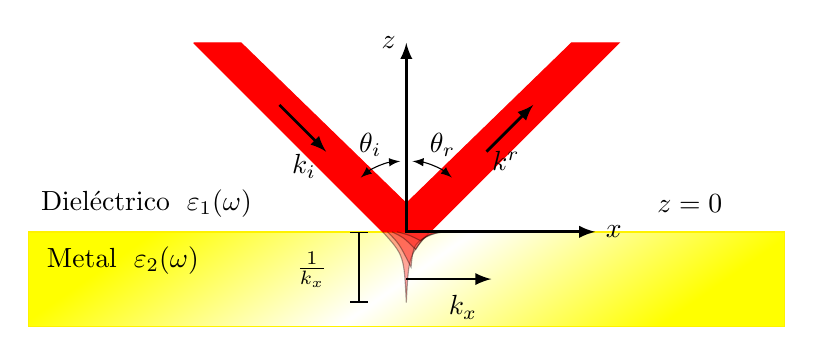
\begin{tikzpicture}[scale=1.2]
	%-------------------------------------------- Incidence media
\shadedraw[	top color = yellow,				%%%%	Color de arriba
			bottom color =yellow,				%%%%	Color de abajo
			middle color = white, 			%%	Color de en medio
			shading angle = 35]			%%%%	Ángulo de gradiente
		 (-4,-1) rectangle (4,0);
% Interface
\draw[yellow,line width=.5pt](-4,0)--(4,0)--(4,-1)--(-4,-1)--(-4,0); %%..5pt, interface]
% Media names
\node at (-2.75,.3) {Diel\'ectrico $\; \varepsilon_1(\omega)$}; 
\node at (-3,-.3) {Metal  $\; \varepsilon_2(\omega)$};
\node at (3,.3) {$z=0$};

%-------------------------------------------- Laser beam outside
\draw[fill=red, opacity = 1,red](-2.25,2)--(-1.75,2)-- (0,.3)  %%% outside the metal
						--(1.75,2)--(2.25,2)
						--(.25,0)--(-.25,0)--(-2.25,2);																														
%--------------------------------------------  Incident Wave
\path (0,0)++(112.5:1cm)node{$\theta_i$};       % Angle
\draw[latex - latex](95:.75cm)arc(95:130:.75cm);
 
    \draw[- latex,line width=1pt](135:1.9cm)--(135:1.2cm);    %Wave vector
    \path (0,0)++(141:1.1cm)node[left]{$\vb{k}_i$};     %Wave vector label
    
%--------------------------------------------  Reflected Wave
\path (0,0)++(67.5:1cm)node{$\theta_r$};       % Angle
\draw[latex - latex](85:.75cm)arc(85:50:.75cm);
 
    \draw[- latex,line width=1pt](45:1.2cm)--(45:1.9cm);    %Wave vector
    \path (0,0)++(43:1.1cm)node[right]{$\vb{k}^r$};     %Wave vector label
  
%--------------------------------------------  Transmitted Wave & Skin depth
\draw[fill = red, opacity = .35] (-.25,0) ..controls (-.025,-.25) .. (0,-.75)
											..controls (.025,-.25) .. (.25,0);  %1st evanescent wave
\draw[fill = red, opacity = .35] (-.2,0) ..controls (-.075,-.125) .. (0.05,-.375)
											..controls (.075,-.125) .. (.3,0);  %2nd evanescent wave
\draw[fill = red, opacity = .35] (-.15,0) ..controls (-.025,-.0625) .. (0.1,-.1875)
											..controls (.175,-.0625) .. (.35,0);  %3rd evanescent wave
\draw[fill = red, opacity = .35] (-.1,0) ..controls (.025,-.03125) .. (0.15,-.09375)
											..controls (.225,-.03125) .. (.4,0);  %4th evanescent wave	

    \draw[- latex,line width=1pt](0,-.5)--(.9,-.5);    %Wave vector
    \node at (.6,-.8) {$\vb{k}_x$};
    
    \draw[|-|,line width=.2mm,black] (-.5,.0)--(-.5,-.75);%
    \node at (-1,-.4) {$\frac{1}{k_x}$};
%--------------------------------------------  Axes
\draw[latex - latex, line width =1pt] (0,2)node[left]{$z$}--(0,0) -- (2,0)node[right]{$x$};
\end{tikzpicture}
	\caption{ Esquema de la interfaz entre un medio dieléctrico y un medio metálico; ambos homogéneos, lineales e isótropos. Un haz de luz incide en el metal desde el medio dieléctrico.  La reflexión es total debido a la naturaleza metálica del material sin embargo, se presenta una onda evanescente que se propaga en dirección paralela a la interfaz.}\label{fig:SPP}
	\end{figure}
	
En la Fig. \ref{fig:SPP} se observa que al incidir el haz en la superficie, en el medio metálico, $z<0$, se presenta una onda evanescente que se propaga en la dirección $\vu{e}_x$, cuya amplitud decae exponencialmente en la dirección $\vu{e}_z$ y cuyo máximo valor $1/k_x$ es la longitud de penetración, con $k_x$ la componente paralela a la interfaz del vector de onda. Si se considera que una onda plana incide, con frecuencia $\omega$ en la dirección $\vb{k}^i$, los campos EMs de la onda evanescente se proponen como 

	\begin{subequations}\eqhalf{	\vb{E}(\vb{r},t) = \vb{E}(z)e^{ik_x x-\omega t },}
	\eqhalf{\vb{H}(\vb{r},t) = \vb{H}(z)e^{ik_x x-\omega t},}
	\label{eq:EHbetax}\end{subequations} \vspace*{-1em}
	
\noindent donde $\vb{E}(z>0)=\vb{E}_1$, con $E_1$ la magnitud de del campo eléctrico dentro del dieléctrico, y $\vb{E}(z<0)=\vb{E}_2$, la magnitud de del campo eléctrico en el medio metálico; la misma distinción se hace para el campo $\vb{H}$ y para la función dieléctrica $\varepsilon(z)$. La ecuación de Helmholtz [Ec. \eqref{eq:Helmholtz}] para los campos EMs de las Ecs. \eqref{eq:EHbetax} son

	\begin{subequations}
	\eqhalf{	\pdv[2]{\vb{E}}{z} + \qty[k_0^2\frac{\varepsilon(z)}{\varepsilon_0} - k_x^2 ] \vb{E}= 0,\label{eq:helmE}}
	\eqhalf{\pdv[2]{\vb{H}}{z} + \qty[k_0^2\frac{\varepsilon(z)}{\varepsilon_0}  - k_x^2 ] \vb{H}= 0, \label{eq:helmH}}
	\end{subequations} 
	
\noindent con $k_0 = \omega/c$. Para el cálculo de la relación de dispersión del SPP, se considera que hay homogeneidad en la dirección $y$, y que la única dependencia en la variable $x$  es en el término de propagación, es decir, que $\partial/\partial x\to ik_x$. Bajo estas consideraciones, al desarrollar la ley de Faraday-Lenz y la ley de Ampère-Maxwell con las expresiones de las Ecs. \eqref{eq:EHbetax} se obtiene el conjunto de ecuaciones \vspace*{-1em}

	\begin{subequations}
	\eqhalf{	\mqty(-\pdv*{E_y}{z} \\ \pdv*{E_x}{z}-ik_x E_z\\ik_x E_y)
				= i\omega\mu_0 \mqty(H_x\\H_y\\h_z),}
	\eqhalf{	\mqty(-\pdv*{H_y}{z} \\ \pdv*{H_x}{z}-ik_x H_z\\ik_x H_y)
				= i\omega\varepsilon(z) \mqty(E_x\\E_y\\E_z).}	
	\end{subequations}\noindent 

El SPP es sensible a la polarización de la onda plana incidente por lo que se consideran los casos de polarización \emph{s} y \emph{p}. En polarización \emph{s}, las componentes no nulas de los campos EMs son $E_y$, $H_z$ y $H_x$, por lo que se  cumplen con las relaciones

	\begin{subequations}
	\eqhalf{	H_x =  \frac{i}{\omega \mu_0} \pdv{E_y}{z},\label{eq:Hx}}
	\eqhalf{H_z =  \frac{k_x}{\omega \mu_0} E_y, \label{eq:Hz}}	
	\label{eq:ondaS}	\end{subequations} \vspace*{-1em}

\noindent junto con la ecuación de Helmholtz para el campo eléctrico [Ec. \eqref{eq:helmE}] con  $\vb{E} = E_y\vu{e}_y$, cuya solución se propone como
	\begin{align}
	E_y(z) = \begin{dcases}
		E_1 e^{ik_x x} e^{-k_{1,z}z}, & z>0\\
		E_2 e^{ik_x x} e^{k_{2,z} z}, & z<0
		\end{dcases},\label{eq:AnsatzEy}
	\end{align}
con $k_{j,z} = k_j\cos\theta_i$ y $k_j = k_0 \sqrt{\varepsilon_j(\omega)/\varepsilon_0}$, con $j = 1,2$; donde se escribe de forma explícita el comportamiento de decaimiento exponencial en la amplitud y se omite el término $e^{-i\omega t}$ por simplicidad. Al calcular el campo $\vb{H}$ con las Ecs. \eqref{eq:ondaS} y \eqref{eq:AnsatzEy}, se obtienen a las expresiones 
	
	\eqhalf{	H_x(z) = \begin{dcases}
	-i \frac{E_1}{\omega\mu_0}k_{1,z} e^{ik_x x} e^{-k_{1,z} 	z}, & z>0\\
	i \frac{E_2}{\omega\mu_0}k_{2,z} e^{ik_x x} e^{k_{2,z} z}, & z<0
	\end{dcases},\notag}
	\eqhalf{	H_z(z) = \begin{dcases}
	\frac{E_1}{\omega\mu_0}k_x  e^{ik_x x} e^{k_{1,z} z} & z>0\\
	\frac{E_2 }{\omega\mu_0}k_x  e^{ik_x x} e^{k_{2,z}z} & z<0
	\end{dcases}.\notag}
	
\noindent   Las condiciones a la frontera impuestas en los campos EMs resultan en que la componente paralela a la interfaz del campo eléctrico, $E_y$, y del campo $\vb{H}$, $H_z$, sean continuas, por lo que $E_1 = E_2$. Adicionalmente, por la continuidad de la componente paralela a la interfaz del  campo $\vb{H}$, $H_x$, se concluye que en $z=0$
	\begin{align}
	E_1\qty(k_{1,z}+k_{2,z})= 0. \label{eq:condS}
	\end{align}
Por el \emph{Ansatz} propuesto en la Ec. \eqref{eq:AnsatzEy}, para que la onda evanescente esté confinada a la interfaz se debe cumplir que $k_{j,z}<0$, por tanto, la Ec. \eqref{eq:condS} se satisface sólo si $E_1 = E_2 = 0$, es decir  que no existe un acoplamiento entre los electrones libres del metal en la interfaz plana y la onda EM incidente para polarización \emph{s}.

El cálculo de la relación de dispersión del SPP para polarización \emph{p} es análogo al cálculo con polarización \emph{s} al intercambiar el campo eléctrico por el campo $\vb{H}$ y al intercambiar la permitividad magnética por la función dieléctrica \cite{maier2007plasmonics}, es decir, $\vb{E}\leftrightarrow\vb{H}$ y $\varepsilon(z)\leftrightarrow\mu_0$. Al considerar las condiciones de continuidad del campo $\varepsilon(z)\vb{E}$ y el campo $\vb{H}$ se obtiene la expresión
	\begin{align*}
	\frac{E_1}{\omega}\qty( \frac{k_{1,z}}{\varepsilon_1}+  \frac{k_{2,z}}{\varepsilon_2} ) = 0,
	\end{align*}
que lleva a la condición
	\begin{align}
	\frac{k_{1,z}}{k_{2,z}} = - \frac{\varepsilon_1}{\varepsilon_2}. \label{eq:condP}
	\end{align}
Asimismo, la ecuación de Helmholtz para el campo $\vb{H}$ [Ec. \eqref{eq:helmH}] impone que
	\begin{align}
	k_{j,z}^2 = k_x^2 - k_0^2 \frac{\varepsilon_j}{\varepsilon_0}.
	\label{eq:kdkm}
	\end{align}
Al elevar al cuadrado los dos miembros de la Ec. \eqref{eq:condP}, sustituir $k_{j,z}^2$ con la Ec. \eqref{eq:kdkm}, y  despejar $k_x^2$  empleando la identidad de diferencia de cuadrados,  se calcula la relación de dispersión del SSP. Adicionalmente, como  $k_0^2 \varepsilon_j(\omega)= k_x^2 +k_{j,z}^2$, entonces\cite{maier2007plasmonics}\vspace*{-.75em}\begin{subequations}
	\begin{tcolorbox}[title = Relación de dispersión del SPP, breakable ]
	\eqhalf{k_x^2 = \frac{k_0^2}{\varepsilon_0} \frac{\varepsilon_1 \varepsilon_2}{\varepsilon_1 + \varepsilon_2},
	\label{eqs:kx}}
	\eqhalf{	k_{j,z}^2 = \frac{k_0^2}{\varepsilon_0} \frac{\varepsilon_j^2}{\varepsilon_1 + \varepsilon_2},\label{eqs:kz}}
	
	con $j=1$, el medio dieléctrico; y $j=2$, el medio metálico.
	\end{tcolorbox}\label{eq:SPPRelDiso}\end{subequations}\vspace*{-.75em}
\noindent
Para que se obtenga una onda evanescente en la interfaz (modo ligado) , $k_x$ debe ser una cantidad real y $k_z$ una cantidad imaginaria \cite{novotny2006principles}, por lo que en la Ec. \eqref{eqs:kx} la suma y el producto de las funciones dieléctricas deben ser ambas positivas o ambas negativas y $\varepsilon_1+\varepsilon_2<0$ en la Ec. \eqref{eqs:kz} \cite{novotny2006principles}, dando como resultado que $\varepsilon_1\varepsilon_2<0$. Estas condiciones se satisfacen con la suposición inicial en la que $\varepsilon_1$ corresponda a la respuesta EM de un medio dieléctrico y $\varepsilon_2$ a la de un metal \cite{maier2007plasmonics,novotny2006principles}. La frecuencia de resonancia $\omega$ del SPP se encuentra cuando las Ecs. \eqref{eq:SPPRelDiso} son máximas, es decir, cuando $\varepsilon_1(\omega)+\varepsilon_2(\omega)$ es mínima. Si se emplea el modelo de Drude-Sommerfeld [Ec. \eqref{eq:Drude}] en el límite $\gamma\to 0$ para $\varepsilon_2(\omega)$, entonces \cite{maier2007plasmonics}  \vspace*{-.75em}
	\begin{tcolorbox}[title =Frecuencia de resonancia del SPP, ams align,  breakable ]
	\omega = \frac{\omega_p}{\sqrt{1+\varepsilon_1/\varepsilon_0}}.
	\end{tcolorbox}\vspace*{-.75em}\noindent

La Fig. \ref{fig:Relaciones_de_dispersion} muestra la relación de dispersión como la dependencia de la frecuencia $\omega$ con componente paralela del vector de onda $k_x$, respecto a una interfaz entre el vacío ($\varepsilon_1=\varepsilon_0$) y un material descrito por le modelo de Drude-Sommerfeld [Ec. \eqref{eq:Drude}] en el límite $\gamma\to 0$ para una onda plana propagándose en el vacío (línea continua negra), para el plasmón de volumen (línea continua roja) y para un SPP (línea continua azul). Las líneas discontinuas roja y azul corresponden a los valores $\omega=\omega_p$ y $\omega=\omega_p/\sqrt{2}$, respectivamente, que son las frecuencias que delimitan el régimen de modos radiativos ($\omega>\omega_p$), donde las dos componentes del vector de onda $\vb{k}$ son cantidades reales, y el régimen de modos ligados ($\omega<\omega_p/\sqrt{2}$), donde $k_x$ es una cantidad real pero la componente del vector de onda perpendicular a la interfaz $k_z$ es una cantidad imaginaria. La línea discontinua negra corresponden a la relación de dispersión de una onda plana propagándose  en un medio con $n=1.5$.

\begin{figure}[h!]\centering
	\begin{tikzpicture}
	\node[inner sep=0pt] at (0,0)
    {\includegraphics[scale=1]{1-Teoria/figs/1-4-RelacionDispersion.pdf}};
    \draw [thick, decorate, decoration={brace,amplitude=10pt,mirror}]
(6.5,-.8) -- (6.5,4.0);
\node at (8,2.5){\footnotesize Modo};
\node at (8,2.){\footnotesize radiativo};
\node at (8,1.5){\footnotesize $k_x\to\text{Real}$};
\node at (8,1.){\footnotesize $k_z\to\text{Real}$};
    \draw [thick, decorate, decoration={brace,amplitude=10pt,mirror}]
(6.5,-3.25) -- (6.5,-1.3);
\node at (8,-1.5){\footnotesize Modo};
\node at (8,-2.){\footnotesize ligado};
\node at (8,-2.5){\footnotesize $k_x\to\text{Real}$};
\node at (8,-3.){\footnotesize $k_z\to\text{Imaginario}$};
\end{tikzpicture}
\vspace*{-1em}
	\caption{Relación de dispersión en términos de $\omega/\omega_p$ como función de $k_xc/\omega_p$ de una onda plana en vacío (línea sólida negra), del plasmón de volumen (línea sólida roja) y del SPP (línea sólida azul) para materiales con una función dieléctrica tipo Drude en el límite $\gamma\to 0$ y sobre una interfaz con el vacío ($\varepsilon_1 =\varepsilon_0$). El régimen de modos radiativos se encuentra en $\omega_p\leq\omega$ (igualdad denotada por la línea discontinua roja), donde $k_x$ y $k_z$ son cantidades reales; el régimen de modos ligados se encuentra en $\omega\leq\omega_p/\sqrt{2}$ (igualdad denotada por la línea discontinua azul), donde $k_x$ es una cantidad real pero $k_z$ es una cantidad imaginaria. Para excitar a SPP es necesario cambiar el índice de refracción de la matriz, por ejemplo empleando un prisma para obtener una onda plana viajando en vidrio (línea punteada negra); la región sombreada delimita las frecuencias a las que el SPP puede excitarse.}
	\label{fig:Relaciones_de_dispersion}
	\end{figure}		

La relación dispersión de la onda plana propagándose en el vacío (línea continua negra en la Fig. \ref{fig:Relaciones_de_dispersion})  es igual a la del SPP (línea continua azul) para  $k_x=0$, por lo que no es posible excitar al SPP con este tipo de ondas \cite{trugler2011properties}. Sin embargo, es posible excitar al SPP empleano un tercer medio dieléctrico, con una función dieléctrica mayor al del dieléctrico que forma la interfaz con el medio metálico donde se excitará el SPP \cite{trugler2011properties}. Un método experimental, pero no el único \cite{maier2007plasmonics}, para excitar al SPP sobre la interfaz formada por una placa metálica con una función dieléctrica $\varepsilon_2(\omega)$ y la matriz dieléctrica con $\varepsilon_1(\omega)$, donde se encuentra inmersa la placa, al emplear una configuración de reflexión total atenuada (Atenuatted Total Reflexión, ATR) \cite{kabashin2009plasmonic}, en donde una onda evanescente interactúa con un objeto \cite{hecht1998optics}, como puede ser una segunda interfaz o bien, NPs soportadas sobre el sustrato. En la Fig. \ref{fig:ATR-SPP} se muestra una posible configuración para excitar experimentalmente al SPP mediante la medición de la reflectancia y el cálculo de los valores que se obtendrían en el experimento. El arreglo consiste en una  placa metálica, con una función dielétrica $\varepsilon_2(\omega)$ y altura $d$, inmersa en un dieléctrico $\varepsilon_1(\omega)=\varepsilon_0$ sobre un sustrato cuya función dieléctrica $\varepsilon_3(\omega)$ cumpla con $\varepsilon_3(\omega)>\varepsilon_1(\omega)$; en la Fig. \ref{sfig:ATR} el sustrato empleado es un prisma con $\varepsilon_3(\omega)/\varepsilon_0=1.5^2$. Cuando una onda plana incide sobre la interfaz entre la placa metálica y el sustrato, se produce una onda evanescente que se propaga en la dirección $\vb{k}_x=k_x\vu{e}_x$ y si $1/k_x>d$, la onda evanescente penetra la interfaz entre la matriz y la placa, excitando al SPP sobre esta interfaz \cite{trugler2011properties}, que se representa como la línea naranja en la Fig. \ref{sfig:ATR}. En la Fig. \ref{sfig:SPP-R} se grafica la reflectancia $R$ como función del ángulo de incidencia $\theta_i$, de la longitud de onda $\lambda$ y la energía $\hbar\omega$, cuando una onda plana se propaga a través del prisma, con $\varepsilon_3(\omega)/\varepsilon_0 = 1.5^2$, e incide sobre una placa de oro de altura $d=45$ nm inmersa en una matriz con $\varepsilon_1(\omega)/\varepsilon_0 = 1$. Para $\lambda<500$ nm la reflectancia es cercana a cero pues el oro se comporta como un dieléctrico, mientras que para $\lambda>500$ nm tiene una respuesta metálica por lo que la reflexión de luz aumenta; para $\theta_i>42^\circ$ la luz que incide sobre la placa metálica se refleja totalmente a excepción de una región con forma de parábola (líneas punteadas blancas). La región donde $R\approx 0$ en $\lambda>500$ nm corresponde a las combinaciones de ángulo de incidencia y longitudes de onda --equivalente a valores de $k_x$ y $\omega$, respectivamente-- a los que el SPP se propaga sobre la interfaz entre la placa de oro y el dieléctrico con $\varepsilon_1(\omega)/\varepsilon_0 = 1$.
			
	\begin{figure}[h!]\centering
	\begin{subfigure}{.01\linewidth}\caption{}\label{sfig:ATR}\vspace{5.5cm}\end{subfigure}
	\begin{subfigure}{.45\linewidth}\hspace*{-1.5em}
		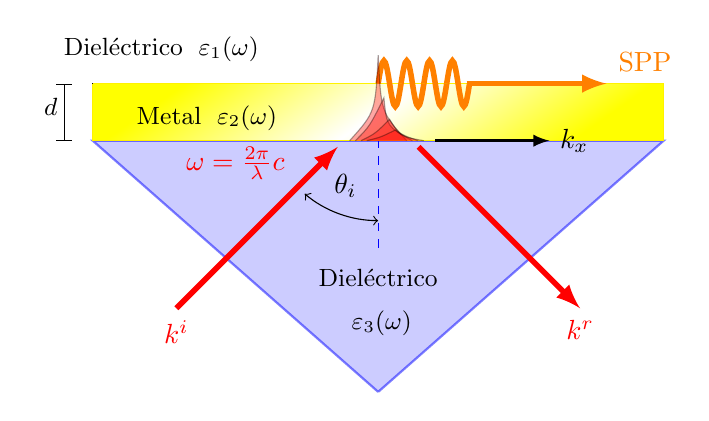
\begin{tikzpicture}[scale= 1.45]
	%-------------------------------------------- Incidence media
\def\a{.3}
\def\d{.3}
\def\dd{.2}
\def\l{2.5}
\def\ll{.05}

\fill[blue, opacity = .2] (0,-\l)--(\l,-\d)--(-\l,-\d);
\draw[blue, opacity = .5,thick] (0,-\l)--(\l,-\d)--(-\l,-\d)--(0,-\l);


\draw[|-|](-\l-.25,-\d)--(-\l-.25,+\dd);
\node at (-\l-.4,0) {\small $\;d$};
\draw[blue, dashed] (0,0)--(0,-\l*.5);

\path (0,0)++(-90-45*.5:\l*.3)node{$\theta_i$};       % Angle
\draw[<->](-90:\l*.4)arc(-90:-90-45*.89:\l*.4);

%\foreach \x in {-4,-2.9,-1,.1,1.2,2.4,3.8}{
%\fill[ball color=yellow, opacity=1] (\x,0) circle(\a);}

\shadedraw[	top color = yellow,				%%%%	Color de arriba
			bottom color =yellow,				%%%%	Color de abajo
			middle color = white, 			%%	Color de en medio
			shading angle = 35]			%%%%	Ángulo de gradiente
		 (-\l,-\d) rectangle (\l,\dd);
% Interface
\draw[yellow,line width=.5pt](-\l,\dd)--(\l,\dd)--(\l,-\d)--(-\l,-\d)--(-\l,\dd); %%..5pt, interface]

% Media names
\node at (0,-1.5) {\small Diel\'ectrico}; 
\node at (0,-1.9) {\small $\; \varepsilon_3(\omega)$}; 
\node at (-1.5,-.1) {\small Metal  $\; \varepsilon_2(\omega)$};
\node at (-1.9,.5) {\small Diel\'ectrico $\; \varepsilon_1(\omega)$}; 


\draw[latex -, thick, red, line width = 2](225:.5)--(225:2.5) node[anchor= north]{$\vb{k}^i$};
\node at (-1.25,-.5) {\color{red} $\omega =\frac{2\pi}{\lambda}c$};
\draw[- latex, thick, red, line width= 2](-45:.5)--(-45:2.5)node[anchor=north ]{$\vb{k}^r$};
\draw[- latex, thick,   line width = 1](.5,-\d)--(1.5,-\d) node[anchor= west ]{$\vb{k}_x$};

\foreach \i in {0,4,8,12}{
\draw[thick, orange,line width = 2,] (\i*\ll,\dd) sin (\i*\ll+\ll,\dd*2) cos (\i*\ll+2*\ll,\dd) sin (\i*\ll+3*\ll,0) cos (\i*\ll+4*\ll,\dd);
}
\draw[- latex, thick, orange,  line width = 2](15.5*\ll,\dd)--(2,\dd) node[anchor= south west ]{SPP};



\draw[fill = red, opacity = .35] (-.25,-\d) ..controls (-.025,.25-\d) .. (0,.75-\d)
											..controls (.025,.25-\d) .. (.25,-\d);  %1st evanescent wave
\draw[fill = red, opacity = .35] (-.2,0-\d) ..controls (-.075,.125-\d) .. (0.05,.375-\d)
											..controls (.075,.125-\d) .. (.3,0-\d);  %2nd evanescent wave
\draw[fill = red, opacity = .35] (-.15,0-\d) ..controls (-.025,.0625-\d) .. (0.1,.1875-\d)
											..controls (.175,.0625-\d) .. (.35,0-\d);  %3rd evanescent wave
\draw[fill = red, opacity = .35] (-.1,0-\d) ..controls (.025,.03125-\d) .. (0.15,.09375-\d)
											..controls (.225,.03125-\d) .. (.4,0-\d);  %4th evanescent wave	


\end{tikzpicture}	
\end{subfigure}\hspace*{2em}
\begin{subfigure}{.01\linewidth}\caption{}\label{sfig:SPP-R}\vspace{5.5cm}\end{subfigure}
	\begin{subfigure}{.45\linewidth}\hspace*{-1em}
	\includegraphics[scale=.73]{1-Teoria/figs/SPP.png}%
	\includegraphics[scale=.73, trim={00 -15 00 00}, clip]{2-Resultados/figs/0-RBar_v}
	\end{subfigure}\hfill	\vspace*{-.7em}
	\caption{\textbf{a)} Esquema de una configuración ATR para la medición de la relación de dispersión del SPP mediante la reflectancia $R$ y \textbf{b)}  cálculo de la reflectancia al considerar una placa de oro con una función dieléctrica $\varepsilon_2(\omega)$, dada por los datos experimentales de \cite{johnson1972constants},	inmersa en una matriz dieléctrica con $\varepsilon_1(\omega)/\varepsilon_0 = 1$ y sobre un prisma dieléctrico con $\varepsilon_3(\omega)/\varepsilon_0=1.5^2$. Cuando un haz de luz con polarización \emph{p} incide sobre la interfaz entre el prisma y la placa de oro a un ángulo mayor al crítico se produce una onda evanescente propagante en la dirección $\vb{k}_x=k_x\vu{e}_x$; si la longitud de penetración $1/k_x$ es mayor a la altura $d$ de la placa metálica, es posible excitar al SPP sobre la interfaz entre el medio metálico y el segun, como se observa en la Fig. \ref{fig:Relaciones_de_dispersion}. En la Fig. \ref{sfig:SPP-R} la línea punteada blanca corresponde a la relación de dispersión del SPP propagándoce sobre la interfaz entre el aire y una placa metálica de oro.}\label{fig:ATR-SPP}
	\end{figure}			
		
		
Los SPPs son ondas electromagnéticas propagantes acopladas a los electrones libres de un metal sobre una interfaz plana e infinita entre el metal y un medio dieléctrico \cite{maier2007plasmonics}. Cuando la interfaz  entre el medio metálico y el dieléctrico tiene una área finita, como sucede con NPs, el resultado de la interacción entre una onda plana incidente y los electrones libres del metal es una excitación no propagante, también causada por el acoplamiento entre la radiación EM y los electrones libres, denominada plasmón de superficie localizado (Localized Surface Plasmon, LSP) \cite{maier2007plasmonics}. La curvatura de las NPs tiene dos efectos en los LSPs: la amplificación de los campos EMs dentro y fuera de la NP (en límite de campo cercano) y la excitación del LSP con iluminación directa, es decir, 
sin emplear métodos como la iluminación en ATR u otros \cite{maier2007plasmonics}.

Al considerar que las NPs son esféricas, se puede emplear la solución de Mie para los campos EMs incidentes ($\vb{E}^i$, $\vb{H}^i$), dados por las Ecs. \eqref{eq:EHiAEV}, y los esparcidos ($\vb{E}^s$, $\vb{H}^s$) por la NP,  dados por las Ecs. \eqref{eq:EHsAEV} y \eqref{eq:MieCoef}. Los campos EMs fuera de la NP son la suma de los campos EMs incidentes y esparcidos, por lo que el vector de Poynting [Ec. \eqref{eq:Poynting}], al considerar su promedio temporal, puede escribirse como \cite{bohren1998absorption}
%
\begin{align*}
\langle\vb{S}\rangle_t 
		= \underbrace{\frac12 \Re \qty(\vb{E}^i\times\vb{H}^{i*})}_{\text{\normalsize $\langle\vb{S}^i\rangle_t $}} + 
		\underbrace{\frac12 \Re \qty(\vb{E}^s\times\vb{H}^{s*})}_{\text{\normalsize $\langle\vb{S}^s\rangle_t $}}+
		\underbrace{	\frac12 \Re\qty(\vb{E}^i\times\vb{H}^{s*} + \vb{E}^s\times\vb{H}^{i*})}_{\text{\normalsize$\langle\vb{S}^{ext}\rangle_t $}},
\end{align*}
%
en donde $\vb{S}^i$ y $\vb{S}^s$ son los vectores de Poynting correspondientes a la onda plana incidente, con número de onda $k_m$ y cuyo campo eléctrico tiene amplitud $E_0$, y a los campos EMs esparcidos por la NP, respectivamente, y $\vb{S}^{ext}$ corresponde a los productos cruzados de estos. Le energía $W_{abs}$ trasportados por los campos EM que es absorbida por la NPs se calcula al integrar $\langle\vb{S}\rangle_t$ sobre una esfera de radio $R$ concéntrica a la NP, cuyo radio sea mayor al radio de la NP, es decir,
%
\begin{equation}
W_{abs} = - \int_0^{2\pi}\int_0^{\pi}
		\qty(\langle\vb{S}^i\rangle_t +\langle\vb{S}^s\rangle_t 
				+\langle\vb{S}^{ext}\rangle_t )
		\cdot \vu{e}_r \dd a
		 = W_i-W_{sca}+W_{ext},
		 \label{eq:WaAll}
\end{equation}
%
donde $W_i = 0$, pues se asume que la matriz donde se encuentra inmersa la NP no es absorbente \cite{bohren1998absorption}. Como $W_{abs}$ es independiente de $R$, al suponer que tanto la matriz como la NP no son magnéticas, es posible emplear la expresión de $\vb{E}^s$ en el de campo lejano dada por las Ecs. \eqref{eq:EHsFF} y a partir de ésta calcular $\vb{H}^s$ con ley de Faraday-Lenz [Ec. \eqref{seq:FLArm}], dando como resultado que $W_{sca}$ se calcula como \cite{bohren1998absorption}
 	\begin{equation}
W_{sca} = \frac{\pi\norm{E_0}^2}{\omega\mu_0 k_m}
		\sum_\ell^\infty (2\ell+1)\Re(-i\xi_\ell^*\xi_\ell')\qty(\abs{a_\ell}^2+\abs{b_\ell}^2),
	\label{eq:WsAll}
	\end{equation}
en donde $a_\ell$ y $b_\ell$ son los coeficientes de Mie [Ecs.  \eqref{eq:MieCoef}], $\xi_\ell(\rho) = \rho h_\ell^{(1)}(\rho)$ una función de Riccati-Bessel, y donde además se emplearon las propiedades de ortogonalidad de las funciones $\sin\varphi$ y $\cos\varphi$ [Ec. \eqref{eq:ortSinCos}], de $\tau_\ell\pm\pi_\ell$ [Ec. \eqref{eq:ortTauPi}], junto con la relación \cite{bohren1998absorption}
	\begin{equation*}
	 \int_{-1}^{1}\qty[\pi_\ell(\mu)\pi_{\ell'}(\mu) + \tau_\ell(\mu)\tau_{\ell'}(\mu)]\dd\mu
 			= \delta_{\ell,\ell'} \frac{2\ell^2(\ell+1)^2}{2\ell+1}.
	 \end{equation*} 
Definiendo la función de Racatti-Bessel $\chi_\ell (\rho) = -\rho y_\ell(\rho)$, se reescribe $\xi_\ell$ como $\xi_\ell= \psi_\ell-i\chi_\ell$, con $\psi_\ell(\rho) = \rho j_\ell(\rho)$. Dado que se cumple que $\chi_\ell\psi_\ell'-\psi_\ell\chi_\ell = 1$ \cite{bohren1998absorption}, y como $\psi_\ell$ y $\chi_\ell$ son funciones reales con variables reales, se obtiene que
\begin{equation*}
\Re(-i\xi_\ell^*\xi_\ell')=\Re\qty[(\chi_\ell^*\psi_\ell'-\psi_\ell^*\chi_\ell')
						-i(\psi\ell^*\psi_\ell'-\chi_\ell^*\chi_\ell') ] 
						= (\chi_\ell^*\psi_\ell'-\psi_\ell^*\chi_\ell') 
						= \chi_\ell\psi_\ell'-\psi_\ell\chi_\ell = 1.
\end{equation*}
Al sustituir $\Re(-i\xi_\ell^*\xi_\ell') = 1$ en la Ec. \eqref{eq:WsAll}, la energía transportada por los campos EMs esparcidos, por unidad de tiempo, es
\begin{equation}
W_{sca} = \frac{\pi\norm{E_0}^2}{\omega\mu_0 k_m}
		\sum_\ell^\infty (2\ell+1) \sum_\ell^\infty\qty(\abs{a_\ell}^2+\abs{b_\ell}^2) = I_i \frac{2\pi}{k_m^2}  \sum_\ell (2\ell+1) \qty(\abs{a_\ell}^2+\abs{b_\ell}^2),
\end{equation}
en donde $I_i = \norm{\langle\vb{S}^i\rangle} = \norm{E_0}^2k_m/2\omega\mu_0$ es la irradiancia, o energía por unidad de tiempo y unidad de área, transportada por la onda plana incidente. Al escribir los campos EM incidentes en términos de las funciones $\pi_\ell$ y $\tau_\ell$, se calcula $W_{ext}$ de forma análoga a $W_{sca}$, de donde se obtiene que
\begin{equation}
W_{ext} = I_i \frac{2\pi}{k_m^2}  \sum_\ell^\infty (2\ell+1) \Re(a_\ell + b_\ell).
\end{equation}

De la Ec. \eqref{eq:WaAll}, empleando las expresiones de $W_{sca}$ y $W_{ext}$ es posible calcular la energía absorbida $W_{abs}$ por la NP. Al despejar $W_{ext}$ de la Ec. \eqref{eq:WaAll} se obtiene que $W_{ext} = W_{abs}+W_{sca}$, razón por la que $W_{ext}$ es la energía que se extinguió  mediante la absorción y esparcimiento de luz por la NP. Al normalizar $W_{sca}$ y $W_{ext}$ por la irradiencia de la onda plana incidente $I_i$, se obtienen cantidades con unidades de área, por lo que se conocen como las secciones transversales de extinción $C_{ext}$, absorción  $C_{abs}$ y esparcimiento $C_{sca}$ que se relacionan como \vspace*{-.75em}
	\begin{tcolorbox}[title = {Secciones transversales de extinción, absorción y esparcimiento}, breakable ]
	\begin{equation}
	C_{ext} = C_{abs} + C_{sca},
	\end{equation}	
	\eqhalf{C_{sca} = \frac{2\pi}{k_m^2}  \sum_\ell (2\ell+1) \qty(\abs{a_\ell}^2+\abs{b_\ell}^2),
	\label{eq:Cabs}}
	\eqhalf{C_{ext} = \frac{2\pi}{k_m^2}  \sum_\ell^\infty (2\ell+1) \Re(a_\ell + b_\ell), \label{eqs:Cext}}

	con $a_\ell$ y $b_\ell$, los coeficientes de Mie, dados por la Ec. \eqref{eq:MieCoef}.
	\end{tcolorbox}\vspace*{-.75em} \noindent
Para poder comparar la cantidad de luz extinta por partículas esféricas, se emplean las eficiencias de absorción $Q_{abs}$, esparcimiento $Q_{sca}$ y extinción $Q_{ext}$, que se calculan a través de las secciones transversales de absorción $C_{abs}$, esparcimiento $C_{sca}$ y extinción $C_{ext}$ al normalizarlas por la sección transversal geométrica de la partícula $C_{geo}=\pi a^2$, dando como resultado
\begin{equation}
\frac{C_{ext}}{\pi a^2} = \frac{C_{ext}}{\pi a^2}  + \frac{C_{ext}}{\pi a^2} 
\;\longrightarrow\; 	Q_{ext} = Q_{abs} + Q_{sca}.
\end{equation}

Para una NP esférica, la sección transversal de extinción $C_{ext}$, al igual que los campos EMs esparcidos [Ec. \eqref{eq:EHsFF}]  está en términos de de una expansión multipolar modulada por los coeficientes $a_\ell$ y $b_\ell$ [Ecs.  \eqref{eq:MieCoef}], que dependen, entre otros parámetros, de $N$ que es el cociente del índice de refracción de la partícula $n_p(\omega)$ entre el de la matriz $n_m(\omega)$.  De la Ec.  \eqref{eq:Cabs} se observa que, para un multipolo $\ell$ fijo, la contribución de de los campos EMs en la extinción de luz es máxima  cuando $C_{abs}$ tiene un máximo \cite{maier2007plasmonics}, o bien, cuando el denominador de los coeficientes de Mie es mínimo \cite{novotny2006principles}.  Si se considera que la respuesta óptica de la partícula es 	$\varepsilon_p (\omega) = n_p^2 (\omega)$, y se mantienen constantes el radio $a$ de la NP, el índice de refracción $n_m$ de la matriz y la longitud de onda $\lambda$ de la onda plana incidente, entonces a la frecuencia $\omega_\ell = c (2\pi / \lambda_\ell)$, donde el denominador de las Ecs.  \eqref{eq:MieCoef} es mínimo, se le denomina \emph{modo normal} de orden $\ell$ \cite{bohren1998absorption,maciel2017momentum}.  Los modos normales eléctricos ocurren a las frecuencias en las que se cumple la condición 
	\begin{align}
	\psi_\ell(Nx)\xi_\ell'(x)-N\xi_\ell(x)\psi_\ell'(Nx) = 0. 
	\label{eq:an_resonance}
	\end{align}
Al considerar el límite de partícula pequeña ($x = k_m a\ll 1$) para esferas inmersas en vacío ($n_m=1$), haciendo un desarrollo en serie de Taylor de las funciones de Bessel y Hankel alrededor del origen y sustituyéndolas en la Ec.  \eqref{eq:an_resonance}, se obtiene que los modos normales eléctricos cumplen la relación \cite{maciel2017momentum}
	\begin{align}
	\varepsilon_p(\omega_\ell) = - \frac{\ell+1}{\ell}.  
	\label{eq:NormalModes}
	\end{align}
Si se emplea la función dieléctrica del modelo de Drude-Sommerfeld [Ec.  \eqref{eq:Drude}] para $\omega = \omega_\ell$	y se sustituye en la Ec.  \eqref{eq:NormalModes}, al despejar $\omega_\ell$ tras considerar además el límite $\gamma\to 0$ y de partícula pequeña, la expresión para la frecuencia de resonancia del  modo normal del multipolo $\ell$ es \cite{maciel2017momentum}\vspace*{-.75em}
\begin{tcolorbox}[title =Frecuencia de resonancia del LSP, ams align,  breakable ]
	\frac{\omega_\ell}{\omega_p} = \sqrt{ \frac{\ell}{2\ell+1}}. \label{eq:PPequeña}
	\end{tcolorbox}\vspace*{-.75em}\noindent
Adicionalmente, si se considera la contribución de todos los órdenes multipolares ($\ell\to \infty$), la mayor frecuencia de resonancia es $\omega_\infty = \omega_p/\sqrt{2}$, que corresponde a la SPR de superfice.

Para partículas esféricas de radio arbitrario $a$ con una función dieléctrica dada por el modelo de Drude-Sommerfeld, la frecuencia de resonancia $\omega_\ell$ sufre un corrimiento al rojo debido al tiempo de acomplamiento $a/c$ entre la interacción EM de la esfera y  la densidad de carga inducida que corresponde al plasmón de superficie \cite{aizpurua1998coupling}.  En la Fig.  \ref{fig:NormalModes} se muestran las frecuencias de resonancia $\omega_\ell$ normalizadas respecto a la frecuancia de plasma $\omega_p$, como función del parámetro adimensional $a\omega_p / c$ para los multipolos $\ell = 1,\,2,\,3,\,4$ y $5$. El límite de partícula pequeña [Ec.  \eqref{eq:PPequeña}]	se recupera cuando  $a\to 0$ (lado izquierdo de la gráfica en la Fig.  \ref{fig:NormalModes}).  

	\begin{figure}[h!]\centering
		\includegraphics[scale=1]{1-Teoria/figs/1-4-DrudeMultipoles.pdf}\vspace*{-1em}
	\caption{Frecuencias de resonancia $\omega_\ell/\omega_p$ para una esfera con una función dieléctrica tipo Drude, como función del parámetro adimensional  $\omega_p a / c$, para los multipolos $\ell = 1,2,3$ y $4$. }
	\label{fig:NormalModes}
	\end{figure}		






Para una partícula esférica con una función dieléctrica arbitraria, los modos normales corresponden a frecuencias en donde la sección transvesal de extinción es máxima para contribución multipolar $\ell$ \cite{kreibig1995clusters}. En la Fig. \ref{fig:QextDrude} se grafica la eficiencia de extinción $Q_{ext}$ (línea continua azul) y la de esparcimiento $Q_{abs}$ (línea punteada azul) como función de la longitud de onda $\lambda$ y la energía $\hbar\omega$ para una partícula esférica de radio $a=30$ nm, inmersa en aire ($n_m=1$), con una función dieléctrica tipo Drude [Ec. \eqref{eq:Drude}] con los parámetros $\hbar\omega_p=4.3$ eV y $\hbar\gamma = 0.15$ eV [ver Fig. \ref{sfig:Qext4-30}] y con $\hbar\omega_p=10$ eV y $\hbar\gamma = 0.15$ eV [ver Fig. \ref{sfig:Qext10-30}].  Para determinar los modos normales del campo eléctrico en la partícula se grafican, adicionalmente, las contribuciones multipolares de las eficiencias de extinción $Q_{ext}^{(\ell)}$ para $\ell = 1,\,2$ y $3$, representadas por las líneas discontinuas verde, rosa y cian, respectivamente, en la escala vertical derecha. Cuando $\hbar\omega_p = 4.3$ eV, los modos normales, en términos de la longitud de onda, se excitan a $\lambda^{(1)}= 526$ nm, $\lambda^{(2)}= 462$ nm y $\lambda^{(3)}= 445 $ nm, mientras que para $\hbar\omega_p = 10$ eV se excitan a $\lambda^{(1)}= 265$ nm $\lambda^{(2)}= 211$ nm $\lambda^{(3)}= 195$ nm.

	\begin{figure}[h!]\centering\hspace*{-1.5em}
	\begin{subfigure}{.01\linewidth}\caption{}\label{sfig:Qext4-30}\vspace{3.75cm}\end{subfigure}
	\begin{subfigure}{.45\linewidth}\hspace*{-1.3em}
	\includegraphics[scale=1]{1-Teoria/figs/1-5-Drude4-ExtSca_30.pdf}
	\end{subfigure}
	\begin{subfigure}{.01\linewidth}\caption{}\label{sfig:Qext10-30}\vspace{3.75cm}\end{subfigure}
	\begin{subfigure}{.45\linewidth}\hspace*{-1em}
	\includegraphics[scale=1]{1-Teoria/figs/1-5-Drude10-ExtSca_30.pdf}
	\end{subfigure}\vspace*{-.7em}
	\caption{Eficiencias de extinción $Q_{ext}$ (línea continua azul) y esparcimiento $Q_{sca}$ (línea punteada azul) como función de la energía $\hbar\omega$ para una partícula esférica con una función dieléctrica tipo Drude con los parámetros \textbf{a)} $\hbar\omega_p=4.3$ eV y $\hbar\gamma = 0.15$ eV y \textbf{b)} $\hbar\omega_p=10$ eV y $\hbar\gamma = 0.15$ eV; los resultados se obtuvieronal considerar la contribución de los primeros seis multipolos garantizando convergencia según el criterio de Wimcombe \cite{wimcombre}. La contribución del multipolo $\ell$ en la eficiencia de extinción $Q_{ext}^{(\ell)}$ se grafica en escala logarítmica (eje vertical derecho) como función de la energía $\hbar\omega$ para localizar los modos normales; se consideraron los modos dipolares ($\ell =1$), cuadrupolares ($\ell = 2$) y octopolares ($\ell = 3$), correspondientes a las líneas verdes, rosas y azules, respectivamente.  Cuando $\hbar\omega_p = 4.3$ eV, los modos normales, en términos de la longitud de onda, se excitan a $\lambda^{(1)}= 526$ nm, $\lambda^{(2)}= 462$ nm y $\lambda^{(3)}= 445 $ nm, mientras que para $\hbar\omega_p = 10$ eV se excitan a $\lambda^{(1)}= 265$ nm $\lambda^{(2)}= 211$ nm $\lambda^{(3)}= 195$ nm.}
	\label{fig:QextDrude}
	\end{figure}	

Al considerar el caso con $\hbar\omega_p = 4.3$ eV, la extinción de luz a $2.3$ eV (modo dipolar) se debe no solo al esparcimiento, sino también a la absorción dado que $Q_{ext}>Q_{sca}$; un tercio de la extinción se debe al esparcimiento, y dos tercios a la absorción. De forma distinta, para $\hbar\omega_p = 10$ eV, el esparcimiento de luz predomina en el proceso de extinción de luz a $\hbar\omega= 4.7$ eV (modo dipolar).













	\section{Modelo de esparcimiento coherente}

La solución de Mie en conjunto con la corrección por tamaño a la función dieléctrica para algún material, permite estudiar la respuesta electromagnética de una NP esférica individual, calcular las frecuencias de resonancia de los plasmones localizados de superficie (Localized Surface Plasmons, LSPs), empleados en la espectroscopía \cite{novotny2006principles}, el sensado \cite{jain2008noble} y la litografía \cite{stockman2011nanoplasmonics}. Sin embargo, no siempre es posible emplear la respuesta EM de una partícula individual para la descripción de un sistema compuesto de muchas partículas ---como una monocapa de NPs---, por lo que se han empleado diversos enfoques entre los que se encuentran la aproximación cuasiestática y las teorías de esparcimiento múltiple \cite{reyes2018analytical,barrera2003coherent,pena-gomar2006coherent,garcia2012multiple}. En el caso límite de partícula pequeña, donde el parámetro de tamaño $x=ka\ll 1$, con $k$ el número de onda dentro de la matriz donde se encuentran inmersas las NPs, suponiéndolas esféricas con un radio $a$, es posible emplear  la aproximación cuasiestática, que considera que sólo la excitación dipolar contribuye al campo total \cite{reyes2018analytical}. En partícular,  bajo la aproximación cuasiestática, es posible desarrollar una teroía de medio efectivo para calcular la reflectancia de una monocapa de NPs \cite{pena-gomar2006coherent,barrera1991optical}. Sin embargo, cuando  el parámetro de tamaño es comparable o mayor a la unidad, una teoría de esparcimiento múltiple es necesaria, debido a la excitación de multipolos de ordenes mayores \cite{pena-gomar2006coherent}. El modelo de esparcimiento coherente (Coherent Scattering Model, CSM) toma en cuenta la interacción de esparcidores ante la presencia de un campo eléctrico promedio; este enfoque además incluye la contribución del esparcimiento múltiple debido a la interacción entre las NPs \cite{reyes2018analytical}.
    
    El cálculo de las expresiones para la reflectancia y la transmitancia en el formalismo del CSM considera el campo eléctrico total esparcido por una monocapa de NPs. En general, éste puede descomponerse en una componente coherente ---respuesta promedio con una dirección de propagación bien definida--- y una componente difusa ---causada por las fluctuaciones y cuya propagación se da en todas las direcciones--- \cite{tsang2000scattering}, como se muestra en la Fig. \ref{fig:CSM-Slab}, en donde un arreglo desordenado de NPs inmersas en una matriz se ilumina con una onda plana monocoromática en la dirección $\vb{k}^i$, y en donde las flechas rojas corresponden a los vectores de onda del campo eléctrico esparcido por NPs en la dirección coherente, mientras que las flechas rosas corresponden a los vectores de onda del campo eléctrico esparcido difuso. Para definir los coeficientes de amplitud de reflexión $r$ y transmisión $t$ para una arreglo desordenado de NPs inmersas en una matriz, se toma en cuenta  únicamente la componente coherente al asumir que la cantidad de energía que porta la componente difusa es mucho menor que la coherente \cite{reyes2018analytical}. Para el cálculo de $r$ y $t$, primero se calculan los coeficientes de amplitud de reflexión y transmisión de una monocapa de NPs suspendida en el espacio libre (Free Standing Monolayer, FSM), es decir, inmersa en un medio dieléctrico denominado matriz, seguido del efecto de introducir una interfaz con un medio denominado sustrato. La reflectancia del sistema sustrato-monocapa-matriz se resuelve al considerar  multiples reflexiones en la interfaz entre las superficies dadas por la interfaz sustrato-matriz y monocapa-matriz. 
 
\begin{figure}[h!]\centering
	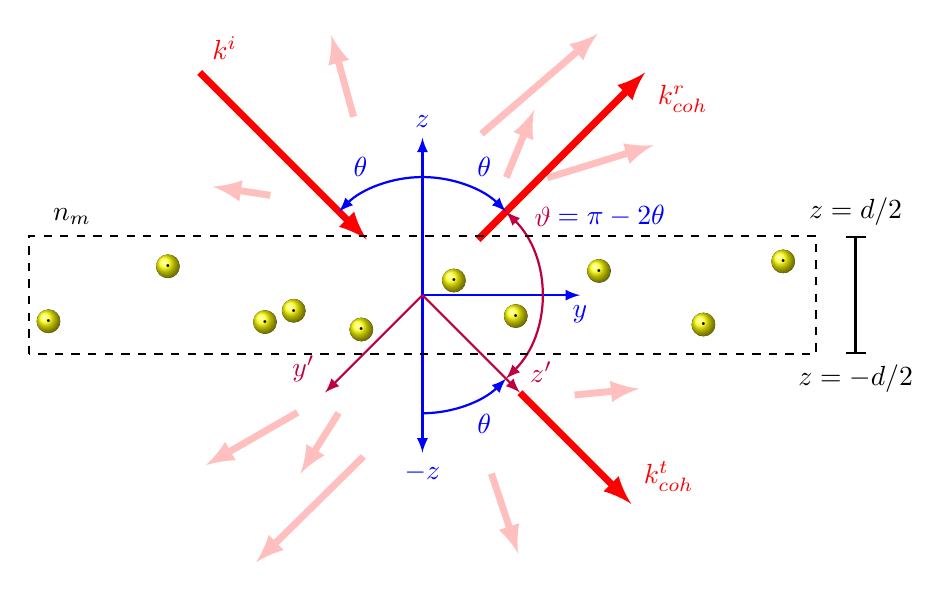
\begin{tikzpicture}[scale=1]
\def\a{.15}
\def\d{.75}
%----------------------NPs--------------
\foreach \y in {-4.5,-3.5,...,3.5,4.5}{
\fill[ball color=yellow, opacity=1] (\y+rand*.5,rand*.45) circle(\a) node[ ]{.};
}

%----------------------difussed scattered field--------------
\begin{scope}[opacity=.25, transparency group]
\foreach \s in {-1,1}{
	\draw[- latex, red, line width=2.5](0,\s*\d)++(25:\s*1.75)--(35+rand*5:\s*3.5);
	\draw[- latex, red, line width=2.5](0,\s*\d)++(35:\s*1.3)--(55+rand*5:\s*2.75);
	\draw[- latex, red, line width=2.5](0,\s*\d)++(165:\s*2)--(155+rand*5:\s*3);
	\draw[- latex, red, line width=2.5](0,\s*\d)++(120:\s*1.75)--(110+rand*5:\s*3.5);
	\draw[- latex, red, line width=2.5](0,\s*\d)++(60:\s*1.5)--(60+rand*5:\s*4);}
\end{scope}

%----------------------coherent scattered field--------------
\draw[latex -, thick, red, line width=2.5](135:1)--(135:4) node[anchor=south west]{$\vb{k}^i$};
\draw[- latex, thick, red, line width=2.5](45:1)--(45:4)node[anchor=north west]{$\vb{k}_{coh}^r$};
\draw[ - latex, thick, red, line width=2.5](-45:1.75)--(-45:3.75) node[anchor=south west]{$\vb{k}_{coh}^t$};

%----------------------Main system--------------
\draw[- latex, thick, blue] (0,0)--(90:2) node[anchor = south]{$z$};
\draw[- latex, thick, blue] (0,0)--(-90:2) node[anchor = north]{$-z$};
\draw[- latex, thick, blue] (0,0)--(0:2) node[anchor = north]{$y$};
\path (0,0)++(135/2:1.5)node[anchor=south west, blue]{$\theta$}; 
\draw[- latex, thick, blue](90:1.5)arc(90:45:1.5);
\path (0,0)++(-135/2:1.5)node[anchor=north west, blue]{$\theta$}; 
\draw[- latex, thick, blue](-90:1.5)arc(-90:-45:1.5);
\path (0,0)++(90+45/2:1.5)node[anchor=south east, blue]{$\theta$}; 
\draw[- latex, thick, blue](90:1.5)arc(90:135:1.5);

----------------------Mie system--------------
\draw[- latex, thick, purple] (0,0)--(-45:1.75) node[anchor = south west]{$z'$};
\draw[- latex, thick, purple] (0,0)--(-135:1.75) node[anchor = south east]{$y'$};
\path (0,0)++(30:1.5)node[anchor=south west, purple]{$\vartheta$}; 
\path (0,0)++(30:1.5)node[anchor=south west, blue]{$\;\;\; =  \pi - 2\theta$}; 
\draw[latex - latex, thick, purple](-45:1.5)arc(-45:45:1.5);

%----------------------thickness and slab-------------
\draw[thick, dashed] (-5,-\d) rectangle (5,\d);
%\draw[thick, dashed] (-5, 0) --  (5,0);
\draw[ |-|, thick,] (5.5,-\d) node[anchor = north]{$z=-d/2$} -- (5.5,\d) node[anchor = south]{$z=d/2$};
\node at (-4.5,1) {$\; n_m$};
\end{tikzpicture}
	\caption{Placa de grosor $d$ y volumen $V$ con $N$ partículas esféricas  idénticas, localizadas al azar e iluminadas con una onda plana monocromática con vector de onda $\vb{k}^i$. La dirección de los campos esparcidos coherentes se denotan por $\vb{k}^r_{coh}$ y $\vb{k}^t_{coh}$. Las flechas rojas sólidas representan las componentes coehrentes del campo esparcido mientras que las rosas represetan la componente difusa. }\label{fig:CSM-Slab}
	\end{figure} 
 
\subsection{Monocapa suspendida en el espacio libre}
 
Para calcular los coeficientes de amplitud de reflexión y transmisión del CSM se calcula el campo eléctrico promedio esparcido por las NPs dentro de la región del espacio, caracterizado por un índice de refracción real $n_m$, delimitada por  $-d/2<z<d/2$, una placa de grosor $d$ y volumen $V$, en donde se encuentran $N$ nanopartículas esféricas idénticas, con índice de refracción $n_p$, y distribuidas espacialmente de forma aleatoria, como se observa en la Fig. \ref{fig:CSM-Slab}. Si una onda plana $\vb{E}^i = E_0 e^{i\vb{k}^i\cdot\vb{r}}\vu{e}_i$ (por simplicidad se omite la dependecia temporal), con $\vu{e}_i$ un vector en el plano de polarización de la onda plana y $|\vb{k}^i| = k = 2\pi n_m /\lambda$, incide sobre la placa, el campo eléctrico esparcido  por las NPs dentro de la placa $\vb{E}^s$ (asumiendo una densidad $N/V$ \emph{baja}), puede calcularse bajo la aproximación de esparcimiento individual (Single Scattering Approximation, SSA), en donde cada NP esparce la luz sin considerar la interacción entre el campo eléctrico esparcido por las otras NPs \cite{barrera2003coherent}. Al considerar la interacción del campo eléctrico incidente con las $N$ NPs dentro de la placa, el campo eléctrico esparcido por todas las partículas tiene componentes espaciales en todas las direcciones, por lo que el campo eléctrico esparcido puede descomponerse en una componente coherente y una difusa, representadas en la Fig. \ref{fig:CSM-Slab} mediante las flechas rojas y rosas, respectivamente.


El  campo eléctrico esparcido promedio $\langle \vb{E}^s\rangle$, que corresponde a la componente coherente, se calcula al considerar el promedio espacial de los campos esparcidos por las NPs dentro de la placa al suponer que la posición de una NPs es independiente de la de las demás y que la probabilidad de encontrar el centro de una NP dentro del volumen de la placa es uniforme, por lo que la componente coherente del campo esparcido es  \cite{garcia2012multiple} 
%
	\begin{align}
	\langle \vb{E}^s\rangle =
	\begin{dcases} 
	      \langle \vb{E}^s_{r,SSA}\rangle e^{i\vb{k}^r_{coh}\cdot\vb{r}} =
	    			i \frac{N}{V}  \frac{d E_0}{2} \frac{\sin(k_z^id)}{k_z^i d} 
				\frac{\mathbb{F}(\vu{k}^r,\vu{k}^i)\cdot \vu{e}_i}{k_z^i }	e^{i\vb{k}^r_{coh}\cdot\vb{r}},									& d/2<z \\
      \langle \vb{E}^s_{t,SSA}\rangle e^{i\vb{k}^t_{coh}\cdot\vb{r}} =
 				i\frac{N}{V} \frac{d E_0}{2}\frac{\mathbb{F}(\vu{k}^i,\vu{k}^i)\cdot \vu{e}_i}{k_z^i}		
				e^{i\vb{k}^t_{coh}\cdot\vb{r}},
							& z<-d/2
   \end{dcases}
   	\label{eq:AvErEt}
	\end{align}
%
en donde $k^i_z = k^i\cos\theta$; $\vb{k}^i$ es el vector de onda del campo eléctrico incidente $\vb{E}^i = \vb{E}_0 e^{i\vb{k}^i\cdot\vb{r}}$, polarizado en la dirección $\vu{e}_i$; $\vb{k}^r_{coh}$ es la dirección de propagación de la componente coherente reflejada; $\vb{k}^t_{coh}=\vb{k}^i$ es la dirección de propagación de la componente coherente transmitida; y $\mathbb{F}$ es el operador de esparcimiento de campo lejano [Ec. \eqref{eq:FarFieldDyadic}] que depende de la dirección de propagación de la onda plana incidente $\vb{k}^i$ y la del campo esparcido $\vb{k}^s$. El término $\mathbb{F}$ no limita la solución del campo eléctrico esparcido promedio al campo lejano, puesto que es un resultado derivado de promediar la respuesta EM \cite{gutierrez2012overview}.

En la Fig. \ref{fig:CSM-Slab} se observa que la dirección de propagación de  $\langle \vb{E}^s_{r,SSA}\rangle$ en $d/2<z$, dada por el vector de onda $\vb{k}^r_{coh}$ y la de $\langle \vb{E}^s_{t,SSA}\rangle$ en  $z<-d/2$, dada por $\vb{k}^t_{coh}$, forman un ángulo $\theta$ respecto a la dirección normal a la monocapa (sitema coordenado azul). A diferencia la componente difusa (flechas rosas), la componente coherente del campo eléctrico esparcido es distinta de cero al calcular el promedio espacial, ya que los campos eléctricos esparcidos por cada NP en la placa interfieren constructivamente en las direcciones de esparcimiento $\vu{k}^s =\vu{k}^i=\vu{k}^t_{coh}$ y $\vu{k}^s =\vu{k}^r_{coh}$ \cite{garcia2012multiple}. Puesto que las NPs dentro de la placa son esféricas e idénticas, se calcula la expresión del operador de esparcimiento $\mathbb{F}(\vu{k}^s,\vu{k}^i)$ al comparar su expresión general [Ec. \eqref{eq:FarFieldDyadic}] con la matriz de esparcimiento de Mie [Ec. \eqref{eq:MieMatrix}], por lo que el operador de esparcimiento de campo lejano es
%
	\begin{align}
	\mathbb{F}(\vu{k}^s,\vu{k}^i) = \frac{1}{-ik} 
	 \mqty(S_2(\vartheta) & 0 \\ 0 & S_1(\vartheta)),
	 \label{eq:FFDydadic-Mie}
	\end{align}
%
en donde $\vartheta$ denota el ángulo entre la dirección del campo esparcido $\vu{k}^s$ y del campo incidente $\vu{k}^i$, con $\vartheta = 0$ para $\vu{k}^s = \vu{k}^t_{coh}$ y $\vartheta = \pi-2\theta$  para $\vu{k}^s = \vu{k}^r_{coh}$, como se observa en la Fig. \ref{fig:CSM-Slab}.
	
Al sustituir la Ec. \eqref{eq:FFDydadic-Mie} en la Ec. \eqref{eq:AvErEt} y multiplicar las expresiones resultantes por $(3ka^3)/(3ka^3)$, con $a$ el radio de las NPs y $k = 2\pi n_m /\lambda$, y agrupar términos, se obtienen las siguientes expresiones 
%
	\begin{subequations}\begin{align}
		\langle \vb{E}^s_{r,SSA}\rangle & = - \frac{E_0}{\cos\theta_i} \frac32  \qty(\frac{N}{V} \frac43\pi a^3)\frac{kd}{(ka)^3}   \frac{\sin(k_z^id)}{k_z^i d}  S_j(\vartheta)\vu{e}_i =
		-\alpha  \frac{\sin(k_z^id)}{k_z^i d}   S_j(\vartheta) \vb{E}_0,
		\label{eqs:EsSSAr}\\
	\langle \vb{E}^s_{t,SSA}\rangle &=  - \frac{E_0}{\cos\theta_i} \frac32
						 \qty(\frac{N}{V}\frac43\pi a^3  ) \frac{kd}{(ka)^3}  S_j(0) \vu{e}_i  
						 = - \alpha S(0) \vb{E}_0,
		\label{eqs:EsSSAt}
	\end{align}\label{eq:EsSSA}\end{subequations}
%
donde  se emplea $j=1$ para polarización $s$ y $j=2$ para $p$ en las entradas no nulas de la matriz de esparcimiento de Mie, $S_j(\vartheta)$, y donde se define $S(0) \equiv S_1(0)=S_2(0)$. La expresión de $\alpha$ en las Ecs. \eqref{eq:EsSSA} en términos del parámetro de tamaño $x=ka$ es
%
\begin{align*}
	\alpha \equiv \frac32 \qty(\frac{N}{V}\frac43 \pi a^3  )\frac{kd}{x^3\cos\theta_i} = \frac32\frac{kd}{ x^3\cos\theta_i} f,
	\end{align*}
%
con $f= N 4\pi a^3/(3V)$ la fracción volumétrica de llenado, que es el cociente entre el volumen que ocupan todas las NPs de la placa entre el volumen de ésta. Si se considera el límite $d\to 0$, lo que equivale a tener una monocapa de partículas esféricas desordenadas y al asumir que la componente difusa del campo esparcido por las partículas es despreciable en comparación a la componente coherente, es posible definir los coeficientes de amplitud de reflexión y transimisión en la SSA a partir de las Ecs. \eqref{eq:EsSSA} como
	
	\begin{subequations}\eqhalf{r_{coh}^{SSA} = -\alpha S_j(\vartheta),}
	\eqhalf{t_{coh}^{SSA} = 1 - \alpha S(0), }
	\label{eqs:rtcohSSA}\end{subequations}\vspace*{-1em}	
	
\noindent considerando para el coeficiente de amplitud de transmisión la contribución de la onda plana incidente en la Ec. \eqref{eqs:EsSSAt}, y al considerar que $V = A d$, con $A$ el área de la monocapa paralela al plano $z=0$, el coeficiente $\alpha$ se reescribe como
%
	\begin{align}
	\alpha = \frac{2\Theta}{x^2 \cos\theta_i},
	\label{eq:alpha}
	\end{align}
%
donde $\Theta = N \pi a^2 / A$ es la fracción de cubierta, que corresponde al área proyectada por las esferas sobre el área de la placa. La distancia mínima promedio $\langle\mathscr{D}_{min}\rangle$ entre las NPs de una monocapa se relaciona con su fracción de cubierta $\Theta$ mediante la expresión $\Theta = \pi a^2 / (2a+\langle\mathscr{D}_{min}\rangle)^2$, como se observa en la Fig. \ref{fig:MeanD}. Entonces, la separación mínima promedio entre las NPs de la monocapa es
	\begin{equation}
	\frac{\langle\mathscr{D}_{min}\rangle}{a} = \sqrt{\frac{\pi}{\Theta}}-2,
	\label{eq:MeanD}
	\end{equation}
de donde se deduce que el valor máximo de $\Theta$ es $0.78$, cuando $\langle\mathscr{D}_{min}\rangle=0$, y que cuando $\langle\mathscr{D}_{min}\rangle= a$ se cumple que $\Theta = \pi/9\approx 0.349$. El cociente entre la distancia mínima promedio entre NPs y su radio se calcula para algunos valores en la Tabla  \ref{tab:meanD}.

\begin{table}[h!] \centering
	\caption{Cociente entre la distancia promedio $\langle\mathscr{D}_{min}\rangle$ entre NPs y su radio $a$, para una monocapa de NPs esféricas e idénticas con fracción de cubierta $\Theta$.}
	\label{tab:meanD}\vspace*{-1em}
	\begin{tabular}{c || c c c c c c c c}
	\hline \hline
	$\Theta$ & $0.05$ & $0.1$ & $0.2$ & $0.3$ & $0.4$ & $0.5$ & $0.6$ & $0.7$\\
 \hline 
	$\langle\mathscr{D}_{min}\rangle / a $& $5.93$ & $3.60$ & $1.96$ & $1.23$ & $0.80$ & $0.51$ & $0.29$ & $0.12$ \\
	\hline \hline
	\end{tabular} 
\end{table}

\begin{figure}[h!]\centering
		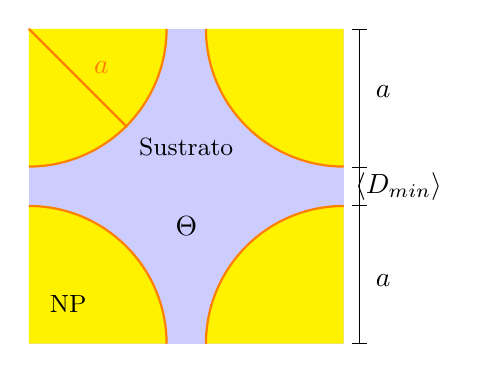
\begin{tikzpicture}[scale=1]
\def	\ll{2}
\def\a{1.75}
%------------------------------------------------ NPs and Substrate
\fill[blue!20] (-\ll,-\ll) rectangle (\ll,\ll);		

\fill[-,yellow,shift ={(-\ll,-\ll)}, opacity = 1](90:\a)arc(90:0:\a)--(0,0)--(90:\a);
\draw[-, orange, thick, shift ={(-\ll,-\ll)}](90:\a)arc(90:0:\a);

\fill[-,yellow,shift ={(-\ll,\ll)}, opacity = 1](-90:\a)arc(-90:0:\a)--(0,0)--(-90:\a);
\draw[-, orange, thick, shift ={(-\ll,\ll)}](-90:\a)arc(-90:0:\a);

\fill[-,yellow,shift ={(\ll,\ll)}, opacity = 1](-90:\a)arc(-90:-180:\a)--(0,0)--(-90:\a);
\draw[-, orange, thick, shift ={(\ll,\ll)}](-90:\a)arc(-90:-180:\a);

\fill[-,yellow,shift ={(\ll,-\ll)}, opacity = 1](90:\a)arc(90:180:\a)--(0,0)--(90:\a);
\draw[-, orange, thick, shift ={(\ll,-\ll)}](90:\a)arc(90:180:\a);

\draw[-, thick, orange] (-\ll,\ll)--(-\ll*.65,\ll*.65) node [anchor = south west]{$a$}--(-.75,.75);
%-------------------------------------------------- media names
\node at (0,.5) {\small Sustrato}; 
\node at (-1.5,-1.5) {\small NP};
\node at (0,-.5) {$\Theta$};

%--------------------------------------------------- dimensions
\draw[-|] (\ll+.2,\ll-\a)--(\ll+.2,\ll);
\node at (\ll+.5, \ll*.6){$a$};

\draw[-|] (\ll+.2,-\ll+\a)--(\ll+.2,-\ll);
\node at (\ll+.5,-\ll*.6){$a$};

\draw[|-|] (\ll+.2,\ll-\a)--(\ll+.2,-\ll+\a);
\node at (\ll+.5, 0){$\;\;\;\;\langle\mathscr{D}_{min}\rangle $};

\end{tikzpicture}
		\caption{ Vista a cero grados desde la normal de una monocapa de NPs de radio $a$ con fracción de cubierta $\Theta$ sobre un sustrato. La separación promedio entre las NPs es $\langle\mathscr{D}_{min}\rangle $, por lo que el área total del cuadrado es $(2a+\langle d \rangle)^2$, el de una NP es $\pi a^2$ y por tanto $\Theta= \pi a^2 / (2a+\langle\mathscr{D}_{min}\rangle )^2$.}\label{fig:MeanD}
	\end{figure}	
	
Al analizar  las Ecs. \eqref{eqs:rtcohSSA} y \eqref{eq:alpha} para ángulos rasantes $\theta\to \pi/2$, se observa que $\alpha\to \infty$, además de que para partículas pequeñas $x\ll 1$ el producto $r_{coh}^{SSA}r_{coh}^{SSA*}$ puede tomar valores mayores a la unidad. Por tanto, los coeficientes de amplitud calculados a partir de la SSA son válidos únicamente para ángulos de incidencia no rasantes  \cite{reyes2018analytical}.

Para calcular los coeficientes de amplitud de reflexión y transmisión para una monocapa de NPs que no estén limitados a ángulos de incidencia bajos, se deben considerar contribuciones de esparcimiento múltiple (Multiple Scattering, MS) en el cálculo del campo eléctrico $\vb{E}^{exc}$  que excita a las partículas dentro de la placa, el cual se puede descomponer como 
	\begin{align}
	\vb{E}^{exc} = \vb{E}^{exc}_{t} e^{i\vb{k}^t_{coh}\cdot\vb{r}}+
					\vb{E}^{exc}_{r} e^{i\vb{k}^r_{coh}\cdot\vb{r}},
	\end{align}
donde  $\vb{E}^{exc}_t$ es la componente del campo eléctrico que excita a las NPs que se transmite según la SSA y $\vb{E}^{exc}_{r}$ la que se refleja; dado que la reflexión y transmisión de $\vb{E}^{exc}$ están dadas por las Ecs. \eqref{eq:EsSSA}, su polarización es la de la onda plana $\vu{e}_i$ y su dirección de propagación está dada por $\vb{k}^t_{coh}$ y $\vb{k}^r_{coh}$, respectivamente. Entonces, el campo eléctrico esparcido promedio considerando el MS $\vb{E}^s_{MS}$, toma en cuenta  las reflexiones y transmisiones de $\vb{E}^{exc}$ según las Ecs. \eqref{eq:EsSSA} en el límite $d\to 0$ \cite{gutierrez2012overview}, como se observa en la Fig. \ref{fig:MScatt-slab-MS}, y la contribución del campo eléctrico incidente $\vb{E}^i$, por lo que  \cite{reyes2018analytical}
%
	\begin{subequations}\begin{align}
		\langle \vb{E}^s_{r,coh}\rangle & =	\langle \vb{E}^s_{r,MS}\rangle
					= \qty[-\alpha S_j(\vartheta)E^{exc}_t -\alpha S(0)E^{exc}_r
					]\vu{e}_i e^{i\vb{k}^r_{coh}\cdot\vb{r}},\\
		\langle \vb{E}^s_{t,coh}\rangle & =\vb{E}^i+\langle\vb{E}^s_{t,MS}\rangle
					= \qty[E_0 -\alpha S(0)E^{exc}_t 
					-\alpha	 S_j(\vartheta)E^{exc}_r
					]\vu{e}_i e^{i\vb{k}^t_{coh}\cdot\vb{r}}.
	\end{align} \label{eqs:EsMS}\end{subequations} \vspace*{-2em}

	\begin{figure}[h!]\centering
		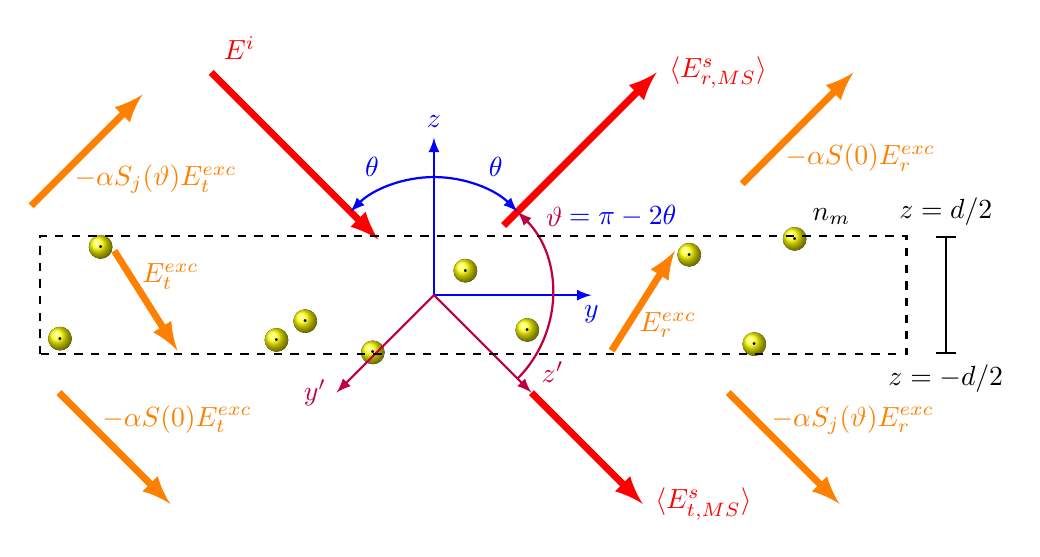
\begin{tikzpicture}[scale=1]
\def\a{.15}
\def\d{.75}

%----------------------NPs--------------
\foreach \y in {-4.5,-4.5,-2.5,-1.5,-.5,.5,1.5,3.5,4,4.5}{
\fill[ball color=yellow, opacity=1] (\y+rand*.5,rand*\d) circle(\a) node[ ]{.};
}

%----------------------averaged fields ---------------------
\draw[latex -, thick, red, line width=2.5](135:1)--(135:4) node[anchor=south west]{$\vb{E}^i$};
\draw[- latex, thick, red, line width=2.5](45:\d+.5)--(45:4)node[anchor=west]{$\langle\vb{E}_{r,MS}^s\rangle$};
\draw[ - latex, thick, red, line width=2.5](-45:1.75)--(-45:3.75) node[anchor=west]{$\langle\vb{E}_{t,MS}^s\rangle$};

%---------------------- Exciting fields ---------------------
\draw[- latex , thick,  orange, line width=2.5,shift ={(-3,0)}](152:1.2)node[anchor= north west]{$\;\;\vb{E}^{exc}_t$}--(250:\d);
\draw[latex - , thick, orange, line width=2.5,shift ={(2,0)}](28:1.2)--(-70:\d) node[anchor= south west]{$\;\;\vb{E}^{exc}_r$};

%-------------- reflected and transmitted exciting fields DOWN ---------------------
\draw[latex - , thick, orange, line width=2.5,shift={(2.5, 0)}](-45:3.75)--(-45:1.75) node[anchor=north west]{$\;\;\;\;-\alpha S_j(\vartheta)\vb{E}^{exc}_r$};
\draw[latex - , thick, orange, line width=2.5,shift={(-6, 0)}](-45:3.75)--(-45:1.75) node[anchor=north west]{$\;\;\;\;-\alpha S(0)\vb{E}^{exc}_t$};

%-------------reflected and transmitted exciting fields UP ---------------------
\draw[latex -, thick, orange, line width=2.5,shift={(2.5, 0)}](45:4)--(45:2)node[anchor=south west]{$\;\;\;\;-\alpha S(0) \vb{E}^{exc}_r$};
\draw[latex -, thick, orange, line width=2.5,shift={(-6, .25)}](45:3.25)--(45:\d+.5)node[anchor=south west]{$\;\;\;\;-\alpha S_j(\vartheta) \vb{E}^{exc}_t$};

%----------------------main system---------------------
\draw[- latex, thick, blue] (0,0)--(90:2) node[anchor = south]{$z$};
\draw[- latex, thick, blue] (0,0)--(0:2) node[anchor = north]{$y$};
\path (0,0)++(135/2:1.5)node[anchor=south west, blue]{$\theta$}; 
\draw[- latex, thick, blue](90:1.5)arc(90:45:1.5);
\path (0,0)++(90+45/2:1.5)node[anchor=south east, blue]{$\theta$}; 
\draw[- latex, thick, blue](90:1.5)arc(90:135:1.5);

%----------------------Mie system---------------------
\draw[- latex, thick, purple] (0,0)--(-45:1.75) node[anchor = south west]{$z'$};
\draw[- latex, thick, purple] (0,0)--(-135:1.75) node[anchor = east]{$y'$};
\path (0,0)++(30:1.5)node[anchor=south west, purple]{$\vartheta$}; 
\path (0,0)++(30:1.5)node[anchor=south west, blue]{$\;\;\; =  \pi - 2\theta$}; 
\draw[- latex, thick, purple](-45:1.5)arc(-45:45:1.5);

%----------------------thickness and slab ---------------------
\draw[thick, dashed] (-5,-\d) rectangle (6,\d);
%\draw[thick, dashed] (-5, 0) --  (6,0);
\draw[ |-|, thick,] (6.5,-\d) node[anchor = north]{$z=-d/2$} -- (6.5,\d) node[anchor = south]{$z=d/2$};
\node at (5,1) {$\; n_m$};
\end{tikzpicture}
		\caption{ Película de grosor $d$ y volumen $V$ con $N$ partículas esféricas idénticas excitada por una onda plana monocromática incidente en la dirección $\vb{k}^i$. El campo eléctrico que excita a las NPs dentro de la película $\vb{E}^{exc}$ se divide en una componente reflejada $ \vb{E}^{exc}_r$ y una transmitida $ \vb{E}^{exc}_t$, considerando así el esparcimiento múltiple por las NPs. Los campos eléctricos esparcidos promedio reflejado $\langle \vb{E}^s_{r,coh}\rangle$ y transmitido $\langle \vb{E}^s_{r,coh}\rangle$ corresponden a la suma  de las Ecs. \eqref{eqs:rtcohSSA} aplicadas a $\vb{E}^{exc}_t$ y a $\vb{E}^{exc}_r$ como se representa en la figura y en las Ecs. \eqref{eqs:EsMS}. Las flechas rojas corresponden a la onda plana incidente y los campos esparcidos promedios mientras que las flechas naranjas corresponden al campo que excita a las NPs. }\label{fig:MScatt-slab-MS}
	\end{figure}	
	
Para determinar la expresión del campo eléctrico que excita a las NPs en la placa $\vb{E}^{exc}$ considerando el MS\footnote{El procedimiento descrito emplea un enfoque heurístico que se publicó en \cite{reyes2018analytical} sin emabargo, un enfoque más riguroso se encuentra en \cite{barrera2003coherent}.}, se divide la placa donde se encuentras las NPs en dos (de grosor $d/2$ cada una) y se calcula el promedio de  $\vb{E}^{exc}$ en la interfaz entre las dos placas ($z=0$) de forma autoconsistente, por lo que las NPs en la placa no sólo son iluminadas por el campo eléctrico incidente $\vb{E}^i$, sino también por $\vb{E}^{exc}$ \cite{reyes2018analytical}. La componente de $\vb{E}^{exc}$ que se transmite, $\vb{E}^{exc}_{t}$, se calcula como la suma del campo eléctrico incidente más el promedio de la transmisión del campo $E^{exc}_t$ y a la reflexión del campo $E^{exc}_r$ ---que corresponden a la suma de los campos esparcidos por las NPs en la placa superior ($0<z<d/2$)--- , es decir,
%
	\begin{subequations}\begin{align}
		\vb{E}^{exc}_t  e^{i\vb{k}^i\cdot\vb{r}}  =
				\qty[E_0  - \frac12 \qty(
					\alpha S(0)E^{exc}_t + \alpha S_j(\vartheta)E^{exc}_r
				)] e^{i\vb{k}^t_{coh}\cdot\vb{r}}  \vu{e}_i,
	\end{align}
%
donde el factor $1/2$ indica que es la respuesta EM promedio dentro de la placa. Asimismo, el campo $\vb{E}^{exc}_{r}$ se calcula como la reflexión  del campo $E^{exc}_t$ y la transmisión del campo $E^{exc}_r$ ---campos esparcidos por las NPs en la placa inferior ($-d/2<z<0$)---, por lo que su expresión es	
%
	\begin{align}
	\vb{E}^{exc}_r  e^{i\vb{k}^r\cdot\vb{r}}  =
				\qty[- \frac12 \qty(
					\alpha S_j(\vartheta)E^{exc}_t + \alpha S(0)E^{exc}_r
				)] e^{i\vb{k}^r_{coh}\cdot\vb{r}}  \vu{e}_i.
	\end{align} \label{eq:Eexc}\end{subequations}
%
En la Fig. \ref{fig:Eexc} se muestra una representación gráfica de las Ecs. \eqref{eq:Eexc}, que són válidas únicamente en $-d/2<z<d/2$.

\begin{figure}[h!]\centering
	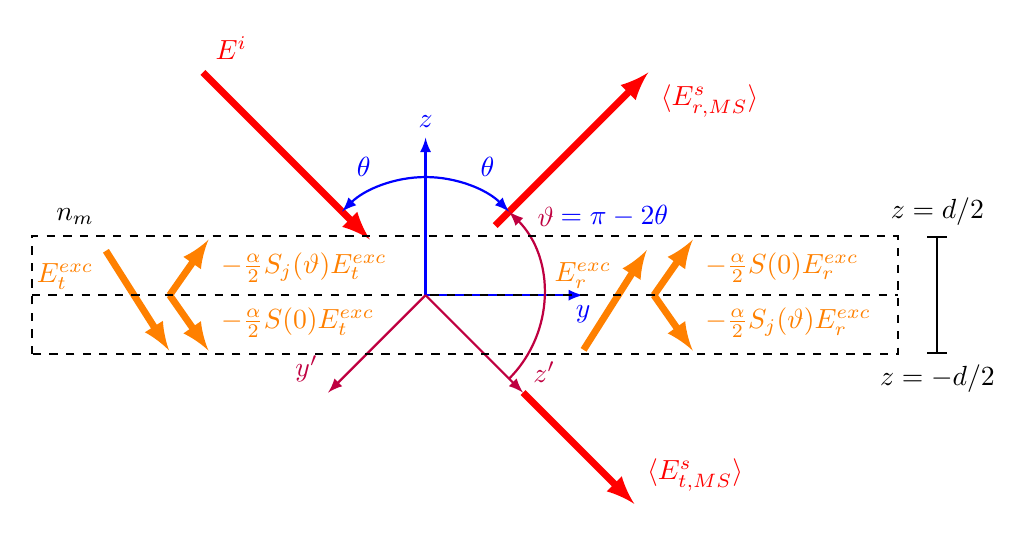
\begin{tikzpicture}[scale=1]
\def\a{.15}
\def\d{.75}

%\foreach \y in {-4.5,-3.5,-2.5,-.5,.5,2.5,3.5,4.5}{
%\fill[ball color=yellow, opacity=1] (\y+rand*.5,rand*\d) circle(\a) node[ ]{.};
%}


\draw[latex -, thick, red, line width=2.5](135:1)--(135:4) node[anchor=south west]{$\vb{E}^i$};
\draw[- latex, thick, red, line width=2.5](45:\d+.5)--(45:4)node[anchor=north west]{$\langle\vb{E}_{r,MS}^s\rangle$};
\draw[ - latex, thick, red, line width=2.5](-45:1.75)--(-45:3.75) node[anchor=south west]{$\langle\vb{E}_{t,MS}^s\rangle$};

%---------------------- Exciting transmitted field ---------------------
\draw[latex - , thick,  orange, line width=2.5,shift={(-3., 0)}](250:\d)--(152:1.2) node[anchor= north east]{$\vb{E}^{exc}_t$};

\draw[- latex , thick,  orange, line width=2.5, shift={(-2.5, 0)}](180:\d)--(250:\d) node[anchor= south west]{$-\frac{\alpha}{2} S(0)\vb{E}^{exc}_t$};
\draw[- latex , thick,  orange, line width=2.5, shift={(-2.5, 0)}](180:\d)--(110:\d) node[anchor= north west]{$-\frac{\alpha}{2} S_j(\vartheta)\vb{E}^{exc}_t$};

%---------------------- Exciting reflected field ---------------------
\draw[- latex , thick, orange, line width=2.5,shift={(1.75, .01)}](-70:\d)--(28:1.2) node[anchor=north east]{$\vb{E}^{exc}_r\;\;\;$};

\draw[- latex , thick,  orange, line width=2.5, shift={(3.65, 0)}](180:\d)--(250:\d) node[anchor= south west]{$-\frac{\alpha}{2} S_j(\vartheta)\vb{E}^{exc}_r$};
\draw[- latex , thick,  orange, line width=2.5, shift={(3.65, 0)}](180:\d)--(110:\d) node[anchor= north west]{$-\frac{\alpha}{2}S(0)\vb{E}^{exc}_r$};

%----------------------Main system---------------------
\draw[- latex, thick, blue] (0,0)--(90:2) node[anchor = south]{$z$};
\draw[- latex, thick, blue] (0,0)--(0:2) node[anchor = north]{$y$};
\path (0,0)++(135/2:1.5)node[anchor=south west, blue]{$\theta$}; 
\draw[- latex, thick, blue](90:1.5)arc(90:45:1.5);
\path (0,0)++(90+45/2:1.5)node[anchor=south east, blue]{$\theta$}; 
\draw[- latex, thick, blue](90:1.5)arc(90:135:1.5);

%----------------------Mie system---------------------
\draw[- latex, thick, purple] (0,0)--(-45:1.75) node[anchor =south west]{$z'$};
\draw[- latex, thick, purple] (0,0)--(-135:1.75) node[anchor =south east]{$y'$};
\path (0,0)++(30:1.5)node[anchor=south west, purple]{$\vartheta$}; 
\path (0,0)++(30:1.5)node[anchor=south west, blue]{$\;\;\; =  \pi - 2\theta$}; 
\draw[- latex, thick, purple](-45:1.5)arc(-45:45:1.5);

%----------------------thickness and slab ---------------------
\draw[thick, dashed] (-5,-\d) rectangle (6,\d);
\draw[thick, dashed] (-5, 0) --  (6,0);
\draw[ |-|, thick,] (6.5,-\d) node[anchor = north]{$z=-d/2$} -- (6.5,\d) node[anchor = south]{$z=d/2$};
\node at (-4.5,1) {$\; n_m$};

\end{tikzpicture}
	\caption{ Película de grosor $d$ y volumen $V$ con $N$ partículas esféricas idénticas (no mostradas en la figura) divida en dos regiones: $z<0$ y $z>0$. Una onda plana monocromática propagándose en la dirección $\vb{k}^i$ incide en las placas, generando un campo eléctrico que excita a las NPs dentro de la película y que considera el esparcimiento múltiple de las NPs al dividirlo en una componente reflejada $\vb{E}^{exc}_r$ y una transmitida $\vb{E}^{exc}_t$, dando como resultado a los campos esparcidos promedio reflejado $\langle\vb{E}_{r,MS}^s\rangle$ y transmitido $\langle\vb{E}_{t,MS}^s\rangle$. Sobre la interfaz entre las dos placas ($z=0$) tanto $\vb{E}^{exc}_r$ como $\vb{E}^{exc}_t$ se reflejan y transmiten según las Ecs. \eqref{eqs:rtcohSSA}, proceso descrito por las Ecs. \eqref{eq:Eexc}. Las flechas rojas corresponden a la onda plana incidente y los campos esparcidos promedios mientras que las flechas naranjas corresponden al campo que excita a las NPs. }\label{fig:Eexc}
	\end{figure}	
	
Al resolver las Ecs. \eqref{eq:Eexc} para $E^{exc}_t$ y $E^{exc}_r$ en términos del campo eléctrico incidente $\vb{E}_0$ se obtienen las siguientes expresiones
%
	\begin{align*}
	\vb{E}^{exc}_t  &= \frac{1+\frac12\alpha S(0)}
				{1+\alpha S(0) +\frac14\alpha^2\qty[S^2(0)-S_j^2(\vartheta)]}\vb{E}_0,\\
	\vb{E}^{exc}_r  &= \frac{-\frac12\alpha S_j(\vartheta)}
				{1+\alpha S(0) +\frac14\alpha^2\qty[S^2(0)-S_j^2(\vartheta)]}\vb{E}_0,
	\end{align*}
%
por lo que, al sustituirlas en las expresiones de los campos esparcidos promedio reflejados y transmitidos [Ecs. \eqref{eqs:EsMS}], se obtienen
%
	\begin{align*}
	\langle \vb{E}^s_{r,coh}\rangle &=
			\frac{-\alpha S_j(\vartheta)}{1+\alpha S(0)+\frac14 \alpha^2 \left[S^2(0)-S_j^2 (\vartheta) \right]} \vb{E}_0 e^{i\vb{k}^r_{coh}\cdot\vb{r}},\\
	\langle \vb{E}^s_{r,coh}\rangle &=
			\frac{1-\frac14\alpha^2\qty[S^2(0)-S_j^2(\vartheta)]}{1+\alpha S(0)+\frac14 \alpha^2 \left[S^2(0)-S_j^2 (\vartheta) \right]} \vb{E}_0 e^{i\vb{k}^t_{coh}\cdot\vb{r}},
	\end{align*}
%
de donde es posible calcular los coeficientes de amplitud de reflexión y transmisión para una monocapa de NPs esféricas bajo el formalismo del CSM. Entonces, considerando que el campo eléctrico que excita a las NPs toma en cuenta el esparcimiento múltiple y que la componente coherente del campo esparcido es mucho mayor que la contribución de la componente difusa, así como $\vartheta = \pi-2\theta$, se obtiene que \vspace*{-.75em}
%
	\begin{subequations}\begin{tcolorbox}[title = Coeficientes de amplitud del CSM, breakable ]
	\begin{align}
	r_{coh}&=\frac{-\alpha S_j(\pi-2\theta)}
				{1+\alpha S(0)+\frac14 \alpha^2 \left[S^2(0)-S_j^2 (\pi-2\theta) \right]},
			\label{seq:rcoh}\\
	t_{coh}&=\frac{1-\frac14\alpha^2\qty[S^2(0)-S_j^2(\pi-2\theta)]}
				{1+\alpha S(0)+\frac14 \alpha^2 \left[S^2(0)-S_j^2 (\pi-2\theta) \right]},
		\label{seq:tcoh}
	\end{align}
	con $j=1$ para polarización $s$, $j=2$ para $p$ y $S(0)=S_1(0)=S_2(0)$.
	\end{tcolorbox}\label{eqs:rtcoh}\end{subequations}\vspace*{-.75em}\noindent

	 \subsection{Monocapa sobre un sustrato}

Las Ecs. \eqref{eqs:rtcoh} corresponden a los coeficientes de amplitud de reflexión y transmisión de una onda plana $\vb{E}^i$ que incide a un ángulo $\theta$ sobre una monocapa de NPs esféricas, idénticas, de radio $a$ e índice de refracción $n_p$, localizadas de forma aleatoria e inmersa en una matriz con índice de refracción $n_m$, sin ser soportada de alguna forma. Sin embargo, en la realidad las NPs no pueden estar suspendidas en un espacio libre, sino que están soportadas sobre un sustrato, de índice de refracción $n_s$; adicionalmente la incidencia del haz de luz puede ser tanto en configuración externa, como se muestra en la Fig. \ref{figs:CSM-Ext}, como en interna, es decir ATR, como se muestra en la Fig. \ref{figs:CSM-ATR}.

	\begin{figure}[h!]\centering
	\begin{subfigure}{.05\textwidth}\vspace{-4.5cm}\caption{}\label{figs:CSM-Ext}\end{subfigure}\hspace*{-2em}
	\begin{subfigure}{.48\textwidth}
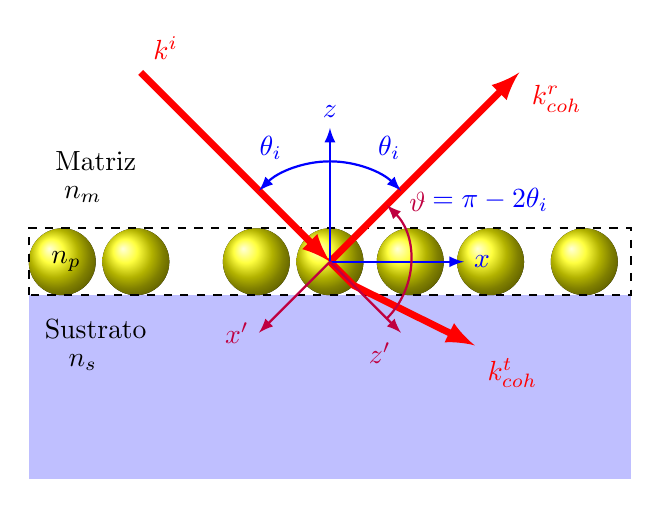
\begin{tikzpicture}[scale=.85]
\def\a{. 5}
\def\d{. 5}

\fill[blue, opacity=. 25] (-4. 5,-6.5*\d) rectangle (4. 5,-\d);

\foreach \x in {-4,-2. 9,-1. 1,0,1. 2,2. 4,3. 8}{
\fill[ball color=yellow, opacity=1] (\x,0) circle(\a);}


\draw[thick, dashed] (-4. 5,-\d) rectangle (4. 5,\d);

\draw[latex -, thick, red, line width=2. 5](135:0)--(135:4) node[anchor=south west]{$\vb{k}^i$};
\draw[- latex, thick, red, line width=2. 5](135:0)--(135:-.5)--(150:-2.5) node[anchor=north west]{$\vb{k}^t_{coh}$};
\draw[- latex, thick, red, line width=2. 5](45:0)--(45:4)node[anchor=north west]{$\vb{k}^r_{coh}$};

\draw[- latex, thick, blue] (0,0)--(90:2) node[anchor = south]{$z$};
\draw[- latex, thick, blue] (0,0)--(0:2) node[anchor = west]{$x$};
\path (0,0)++(135/2:1. 5)node[anchor=south west, blue]{$\theta_i$}; 
\draw[- latex, thick, blue](90:1. 5)arc(90:45:1. 5);
\path (0,0)++(90+45/2:1. 5)node[anchor=south east, blue]{$\theta_i$}; 
\draw[- latex, thick, blue](90:1. 5)arc(90:135:1. 5);

\draw[- latex, thick, purple] (0,0)--(-45:1. 5) node[anchor = north east]{$z'$};
\draw[- latex, thick, purple] (0,0)--(-135:1. 5) node[anchor = east]{$x'$};
\path (0,0)++(30:1. 2)node[anchor=south west, purple]{$\vartheta$}; 
\path (0,0)++(30:1. 2)node[anchor=south west, blue]{$\;\;\; =  \pi - 2\theta_i$}; 
\draw[- latex, thick, purple](-45:1. 2)arc(-45:45:1. 2);



\node at (-3.5,1.5) {Matriz};
\node at (-3.75,1) {$\; n_m$};
\node at (-4,0) {$\; n_p$};
\node at (-3.75,-1.5) {$\; n_s$};
\node at (-3.5,-1) {Sustrato};	
\end{tikzpicture}
	\end{subfigure}
	\begin{subfigure}{.05\textwidth}\vspace{-4.5cm}\caption{}\label{figs:CSM-ATR}	\end{subfigure}\hspace*{-2em}
	\begin{subfigure}{.48\textwidth} 
		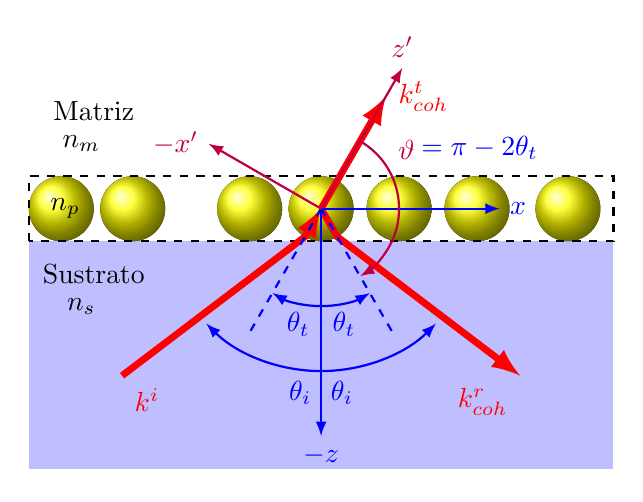
\begin{tikzpicture}[scale=.825]
\def\a{. 5}
\def\d{. 5}

\fill[blue, opacity=. 25] (-4. 5,-8*\d) rectangle (4. 5,-\d);

\foreach \x in {-4,-2. 9,-1. 1,0,1. 2,2. 4,3. 8}{
\fill[ball color=yellow, opacity=1] (\x,0) circle(\a);}


\draw[thick, dashed] (-4. 5,-\d) rectangle (4. 5,\d);

\draw[latex -, thick, red, line width=2. 5](0,0)--(-120:. 5)--(-140:4) node[anchor=north west]{$\vb{k}^i$};
\draw[- latex, thick, red, line width=2. 5](0,0)--(-120:-2)node[anchor=west]{$\vb{k}^t_{coh}$};
\draw[- latex, thick, red, line width=2. 5](0,0)--(-60:. 5)--(-40:4)node[anchor=north east]{$\vb{k}^r_{coh}$};

\draw[- latex, thick, blue] (0,0)--(-90:3. 5) node[anchor = north]{$-z$};
\draw[- latex, thick, blue] (0,0)--(0:2. 75) node[anchor = west]{$x$};

\path (0,0)++(-90:2. 5)node[anchor=north east, blue]{$\theta_i$}; 
\draw[- latex, thick, blue](-90:2. 5)arc(-90:-45:2. 5);
\path (0,0)++(-90:2. 5)node[anchor=north west, blue]{$\theta_i$}; 
\draw[- latex, thick, blue](-90:2. 5)arc(-90:-135:2. 5);

\draw[thick, blue, dashed](0,0) -- (-120:2. 25);
\draw[thick, blue, dashed](0,0) -- (-60:2. 25);
\path (0,0)++(-90-50/2:1. 6)node[anchor=north west, blue]{$\theta_t$}; 
\draw[- latex, thick, blue](-90:1. 5)arc(-90:-60:1. 5);
\path (0,0)++(-90+50/2:1. 6)node[anchor=north east, blue]{$\theta_t$}; 
\draw[- latex, thick, blue](-90:1. 5)arc(-90:-120:1. 5);

\draw[- latex, thick, purple] (0,0)--(60:2.5) node[anchor = south]{$z'$};
\draw[- latex, thick, purple] (0,0)--(150:2) node[anchor =  east]{$-x'$};
\path (0,0)++(30:1. 2)node[anchor=south west, purple]{$\vartheta$}; 
\path (0,0)++(30:1. 2)node[anchor=south west, blue]{$\;\;\; =  \pi - 2\theta_t$}; 
\draw[- latex, thick, purple](60:1. 2)arc(60:-60:1. 2);


\node at (-3.5,1.5) {Matriz};
\node at (-3.75,1) {$\; n_m$};
\node at (-4,0) {$\; n_p$};
\node at (-3.75,-1.5) {$\; n_s$};
\node at (-3.5,-1) {Sustrato};	
\end{tikzpicture}
	\vspace*{-.35em}\end{subfigure}
	\caption{Esquema de la reflexión coherente de una monocapa de NPs esféricas, con índice de refracción $n_p$,  suspendida en un a matriz con índice de refracción $n_m$ y soportada por un sustrato con índice de refracción $n_s$, iluminada en un esquema de \textbf{a)} incidencia externa  y \textbf{b)} en configuración ATR. El sistema coordenado azul, con el eje $z$ paralelo a la dirección normal a la monocapa, define los ángulos de incidencia $\theta_i$, de reflexión y de transmisión $\theta_t$ mediante la ley de la reflexión y la ley de Snell. El sistema coordenado morado, con el eje $z$ paralelo a $\vb{k}^i$ en \textbf{a)} y paralelo a $\vb{k}^t_{coh}$ en \textbf{b)}, se emplea para determinar el ángulo $\vartheta$ (donde se evalúan los elmentos de la matriz de esparcimiento de Mie) en términos de $\theta_i$ o $\theta_t$.}	\label{fig:CSM-Diagrams}	
	\end{figure}	

En las Fig. \ref{fig:CSM-Diagrams}	 se observa que el ángulo $\theta$ a evaluar $r_{coh}$ y $t_{coh}$ en las Ecs. \eqref{eqs:rtcoh} depende del medio por el que incide el campo eléctrico de la onda plana, con dirección $\vb{k}^i$. En incidencia externa, Fig. \ref{figs:CSM-Ext}, la onda plana incide sobre las NPs a un ángulo $\theta_i$ dado que no interactúa con la interfaz matriz-sustrato y no modifica su trayectoria. Por otro lado, en una configuración ATR, Fig. \ref{figs:CSM-ATR}, la onda plana cruza la interfaz sustrato-matriz, por lo que se refracta a un ángulo $\theta_t$ dado por la ley de Snell, e incide a la monocapa en $\theta=\theta_t$. Además de considerar el ángulo con el que la onda plana ilumina a las NPs, se debe calcular la contribución del sustrato en la reflectancia $R$ y transmitancia $T$, que también depende del medio por donde incide la onda plana.

\begin{figure}[b!]\centering
	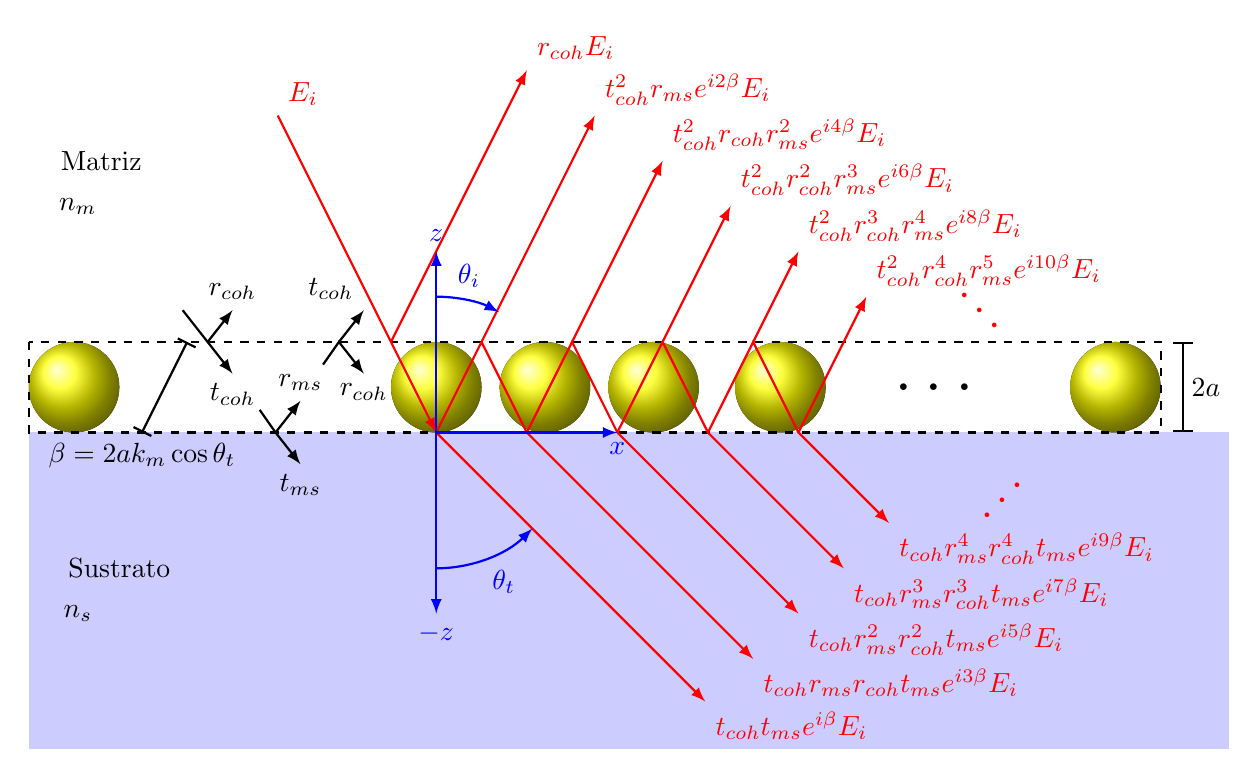
\begin{tikzpicture}[scale=1.15]
\def\a{.5}
\def\d{.5}
\def\t{.3}

\fill[blue, opacity = .2] (-4.5,-3.5) rectangle(8.75,0);

\foreach \x in {-4,0,1.2,2.4,3.8,7.5}{ %-2.9,-1.1
\fill[ball color=yellow, opacity=1] (\x,\d) circle(\a);}

\draw[thick, dashed] (-4.5,2*\d) rectangle (8,0);
\node at (5.5,\d) {\Huge $\ldots$};

%%%%%%%%%%%%%-------------transmisiones

\draw[- latex, thick, red](-135:0)--(-45:4.2) node[anchor=north west]{$t_{coh}t_{ms}e^{i\beta}E_i$};
\draw[- latex, thick, red](0,0)--(1*\d,2*\d)--(2*\d,0)--(3+\d,-3+\d) node[anchor=north west]{$t_{coh}r_{ms}r_{coh}t_{ms}e^{i3\beta}E_i$};
\draw[- latex, thick, red](2*\d,0)--(3*\d,2*\d)--(4*\d,0)--(3+2*\d,-3+2*\d) node[anchor=north west]{$t_{coh}r_{ms}^2r_{coh}^2t_{ms}e^{i5\beta}E_i$};
\draw[- latex, thick, red](4*\d,0)--(5*\d,2*\d)--(6*\d,0)--(3+3*\d,-3+3*\d) node[anchor=north west]{$t_{coh}r_{ms}^3r_{coh}^3t_{ms}e^{i7\beta}E_i$};
\draw[- latex, thick, red](6*\d,0)--(7*\d,2*\d)--(8*\d,0)--(3+4*\d,-3+4*\d) node[anchor=north west]{$t_{coh}r_{ms}^4r_{coh}^4t_{ms}e^{i9\beta}E_i$};
\draw[-, thick, red](8*\d,0)--(9*\d,2*\d);
\node[rotate={45}] at (6.25,-.75) {\color{red}\LARGE $\ldots$};


%%%%%%%%%%%%%-------------reflexiones
\draw[latex -, thick, red](0,0)--(-1.75,3.5) node[anchor=south west]{$E_i$};
\draw[- latex, thick, red](-1*\d,2*\d)--(2-2*\d,4+0*\d) node[anchor=south west]{$r_{coh}E_i$};
\draw[- latex, thick, red](1*\d,2*\d)--(1.75,3.5) node[anchor=south west]{$t_{coh}^2r_{ms}e^{i2\beta}E_i$};
\draw[- latex, thick, red](3*\d,2*\d)--(2+1*\d,4-2*\d) node[anchor=south west]{$ t_{coh}^2r_{coh}r_{ms}^2e^{i4\beta}E_i$};
\draw[- latex, thick, red](5*\d,2*\d)--(2+2.5*\d,4-3*\d) node[anchor=south west]{$ t_{coh}^2r_{coh}^2r_{ms}^3e^{i6\beta}E_i$};
\draw[- latex, thick, red](7*\d,2*\d)--(2+4*\d,4-4*\d) node[anchor=south west]{$ t_{coh}^2r_{coh}^3r_{ms}^4e^{i8\beta}E_i$};
\draw[- latex, thick, red](9*\d,2*\d)--(2+5.5*\d,4-5*\d) node[anchor=south west]{$t_{coh}^2r_{coh}^4r_{ms}^5e^{i10\beta}E_i$};
\node[rotate={-45}] at (6,1.35) {\color{red}\LARGE $\ldots$};



\node at (-4,2.5) {$\; n_m$};
\node at (-3.7,3) {Matriz};
\node at (-4,-2) {$\; n_s$};
\node at (-3.5,-1.5) {Sustrato};

%.55,0
%2,0
%1.2,2*\ḑ
%%\draw[latex - , thick](-2.8,-.5)--(-3.5,.5) node[anchor=north]{$r_{sm},\,t_{sm}$};
\draw[latex - , thick, shift ={(2,2*\d)}](-2.8,-.35)node[anchor=north]{$r_{coh}$}--(-3.075,0)--(-3.25,-.25);
\draw[latex -,thick, shift ={(2,2*\d)}](-2.8,.35)node[anchor=south east]{$t_{coh}$}--(-3.075,0);
\draw[latex - , thick, shift ={(.55,2*\d)}](-2.8,-.35)node[anchor=north]{$t_{coh}$}--(-3.075,0)--(-3.35,.35);
\draw[latex -,thick, shift ={(.55,2*\d)}](-2.8,.35)node[anchor=south]{$r_{coh}$}--(-3.075,0);
\draw[latex - , thick, shift ={(1.3,0)}](-2.8,-.35)node[anchor=north]{$t_{ms}$}--(-3.075,0)--(-3.25,+.25);
\draw[latex -,thick, shift ={(1.3,0)}](-2.8,.35)node[anchor=south]{$r_{ms}$}--(-3.075,0);

\draw[|-|,thick, shift ={(-3.25,0)}](0,0)node[anchor=north]{$\beta = 2ak_m\cos\theta_t$}--(1*\d,2*\d) ;

\draw[|-|,thick, shift ={(8.25,0)}](0,0)--(0,2*\d) ;
\node at (8.5,\d){$2a$};

\draw[- latex, thick, blue] (0,0)--(90:2) node[anchor = south]{$z$};
\draw[- latex, thick, blue] (0,0)--(90:-2) node[anchor = north]{$-z$};
\draw[- latex, thick, blue] (0,0)--(0:2) node[anchor = north]{$x$};
\path (0,0)++(85:1.5)node[anchor=south west, blue]{$\theta_i$}; 
\draw[- latex, thick, blue](90:1.5)arc(90:62.5:1.5);
\path (0,0)++(-70:1.5)node[anchor=north west, blue]{$\theta_t$}; 
\draw[- latex, thick, blue](-90:1.5)arc(-90:-45:1.5);


\end{tikzpicture}
	\caption{ Esquema de las múltiples reflexiones en incidencia externa del sistema matriz-monocapa-sustrato producidos por una onda plana $\vb{E}^i$ que incide sobre una monocapa de NPs esféricas de radio $a$, inmerza en una matriz con índice de refracción  $n_m$ y soportada por un sustrato con índice de refracción $n_s$, a un ángulo $\theta_i$ respecto a la dirección normal de la monocapa. Las reflexiones y transmisiones en la interfaz sustrato-matriz ($z=0$) se describen mediante los coeficientes de amplitud de Fresnel [Ecs. \eqref{eq:rs}--\eqref{eq:tp}], mientras que en la intfaz monocapa-matriz ($z=2a$) las reflexiones y transmisiones son descritas por el CSM [Ecs. \eqref{eqs:rtcoh}]. Los coeficientes de amplitud de reflexión y transmisión se evalúan en $\theta_i$. En los coeficientes de amplitud  $r_{\alpha\beta}$ y $t_{\alpha\beta}$ el medio de incidencia de la onda plana monocromática corresponde a $\alpha$ y el de transmisión a $\beta$.}\label{fig:CSM-externa}
	\end{figure}

Para calcular los coeficientes de amplitud de reflexión y transmisión del sistema matriz-monocapa-sustrato, es decir, en incidencia externa, se consideran las múltiples reflexiones del sistema, mostradas en la Fig. \ref{fig:CSM-externa}. Cuando la onda plana con amplitud $E_i$ incide en la monocapa, en $z=2a$, se presenta una primera reflexión dada por el CSM, es decir que la amplitud del campo eléctrico en la primera reflexión es $r_{coh}E_i$. La segunda reflexión se presenta tras dos transmisiones en la monocapa y una reflexión en la interfaz matriz-sustrato, con una diferencia de fase $2\beta=2(2ak_m\cos\theta)$ respecto a la primera reflexión, es decir, que la amplitud de la segunda reflexión es $t_{coh}^2r_{ms}e^{i2\beta}E_i$. En la tercera reflexión hay dos transmisiones en la monocapa, dos reflexiones en la interfaz matriz-sustrato, y una reflexión en la monocapa; al considerar la diferencia de camino óptico con la primera relfexión, la amplitud de la tercera reflexión es $t_{coh}^2r_{coh}r_{ms}^2e^{i4\beta}E_i$. Al considerar el resto de las reflexiones, se obtiene que el coeficiente de amplitud de reflexión $r$ del sistema es
%
	\begin{align}
	r = r_{coh} +
		 t_{coh}^2r_{ms}e^{i2\beta}+
		 t_{coh}^2r_{coh}r_{ms}^2e^{i4\beta}+
		 t_{coh}^2r_{coh}^2r_{ms}^3e^{i6\beta}+
		 t_{coh}^2r_{coh}^3r_{ms}^4e^{i8\beta}+\ldots
%		 t_{coh}^2r_{coh}^4r_{ms}^5e^{i10\beta}+\ldots\,.
	\label{eq:r_ext_span}
	\end{align}
%
Para el cálculo del coeficiente de amplitud de transmisión $t $ del sistema se sigue un procedimiento análogo al de $r$: la primera transmisión ocurre después de una transmisión en la monocapa, una transmisión en la interfaz matriz-sustrato y una diferencia de fase de $\beta$, por lo que la amplitud de la primera transmisión es $t_{coh}t_{ms}e^{i\beta}$. Para la $m$-ésima transmisión se presentan $m-1$ reflexiones con la monocapa y $m-1$ con el sustrato, además de una fase de $(2m-1)\beta$, es decir,
%
	\begin{align}
	t = t_{coh}t_{ms}e^{i\beta} +
		t_{coh}r_{ms}r_{coh}t_{ms}e^{i3\beta}+
		t_{coh}r_{ms}^2r_{coh}^2t_{ms}e^{i5\beta}+	
		t_{coh}r_{ms}^3r_{coh}^3t_{ms}e^{i7\beta}+ \ldots					
%		t_{coh}r_{ms}^4r_{coh}^4t_{ms}e^{i9\beta}+ \ldots				
%		t_{coh}r_{ms}^5r_{coh}^5t_{ms}e^{i11\beta}+\ldots\,.
	\label{eq:t_ext_span}
	\end{align}\noindent
%	
Al factorizar $r_{ms}t_{coh}^2e^{2i\beta}$ en la Ec. \eqref{eq:r_ext_span}, a excepción del primer término $r_{coh}$, y factorizar $t_{coh}t_{ms}e^{i\beta}$ en la Ec. \eqref{eq:t_ext_span}, se obtienen las expresiones
%
	\begin{align*}
	r &= r_{coh} + r_{ms}t_{coh}^2e^{2i\beta}\left[1+r_{coh}r_{ms}e^{2i\beta}+\qty(r_{coh}r_{ms}e^{2i\beta})^2+\qty(r_{coh}r_{ms}e^{2i\beta})^3+\ldots,\right]\\
	t &= t_{coh}t_{ms}e^{i\beta} \left[1+r_{coh}r_{ms}e^{2i\beta}+\qty(r_{coh}r_{ms}e^{2i\beta})^2+\qty(r_{coh}r_{ms}e^{2i\beta})^3+\ldots\right] ,
	\end{align*}
%
y dado que $\norm{r_{coh}r_{ms}e^{2i\beta}}<1$, es posible reescribir los coeficientes de amplitud del sistema como \vspace*{-.75em}\begin{subequations}
%
	\begin{tcolorbox}[title = Coeficientes de amplitud dados por el CSM en incidencia externa, breakable ]
	\eqhalf{r = r_{coh}(\theta_i)+ \frac{r_{ms}(\theta_i)t_{coh}(\theta_i)e^{i2\beta}}
										{1-r_{coh}(\theta_i)r_{ms}(\theta_i)e^{2i\beta}},
	\label{seq:rCSMext}}
	\eqhalf{t = \frac{t_{ms}(\theta_i)t_{coh}(\theta_i)e^{i\beta}}
									{1-r_{coh}(\theta_i)r_{ms}(\theta_i)e^{2i\beta}},
	\label{seq:tCSMext}}
	
	con $\beta = 2a k_0n_m\cos\theta_i$.
	\end{tcolorbox}\label{eqs:rtCSMext}\end{subequations}\vspace*{-.75em}
%

Cuando se considera que el la onda plana monocromática incide sobre el sistema con un ángulo $\theta_i$ en una confiuración  ATR, ésta se refleja por la interfaz sustrato-matriz ($z=0$) a un ángulo  $\theta_i$ pero se transmite a un ángulo  $\theta_t$. La onda plana ilumina a las NPs a un ángulo $\theta_t$, y a este mismo ángulo se refleja y transmite a través de la monocapa (en $z=2a$), como se observa en la Fig. \ref{fig:CSM-ATR}, donde, por claridad, los subíndices $sm$ corresponden a los coeficientes de Fresnel evaluados en $\theta_i$, mientras que $ms$ y $coh$, en $\theta_t$. De forma análoga al caso de incidencia externa, los coeficientes de amplitud de reflexión y transmisión del sistema son
%
	\begin{align}
	r &= r_{sm}+ 
		t_{sm}r_{coh}r_{ms}e^{i2\beta}+
		t_{sm}r_{coh}^2r_{ms}e^{i4\beta}+
		t_{sm}r_{coh}^3r_{ms}^2e^{i6\beta}+
		t_{sm}r_{coh}^4r_{ms}^3e^{i8\beta}\ldots,
	\label{eq:r_ATR_span}\\		
	t &= t_{sm}t_{coh}e^{i\beta}+ 
		t_{sm}r_{coh}r_{ms}t_{coh}e^{i3\beta}+
		t_{sm}r_{coh}^2r_{ms}^2t_{coh}e^{i5\beta}+
		t_{sm}r_{coh}^3r_{ms}^3t_{coh}e^{i7\beta}+\ldots,	
%		t_{sm}r_{coh}^4r_{ms}^4t_{coh}e^{i9\beta}+\ldots,	
	\label{eq:t_ATR_span}
	\end{align}
donde $\beta = 2ak_m\cos\theta_t$. Al factorizar $t_{sm}r_{coh}t_{ms}e^{2i\beta}$ en la Ec. \eqref{eq:r_ATR_span} y $t_{sm}t_{coh}e^{i\beta}$ en la Ec. \eqref{eq:t_ATR_span}, y considerar que $\norm{r_{coh}r_{ms}e^{i2\beta}}<1$, los coeficientes de amplitud están dados por \vspace*{-2em}

\begin{figure}[h!]\centering
	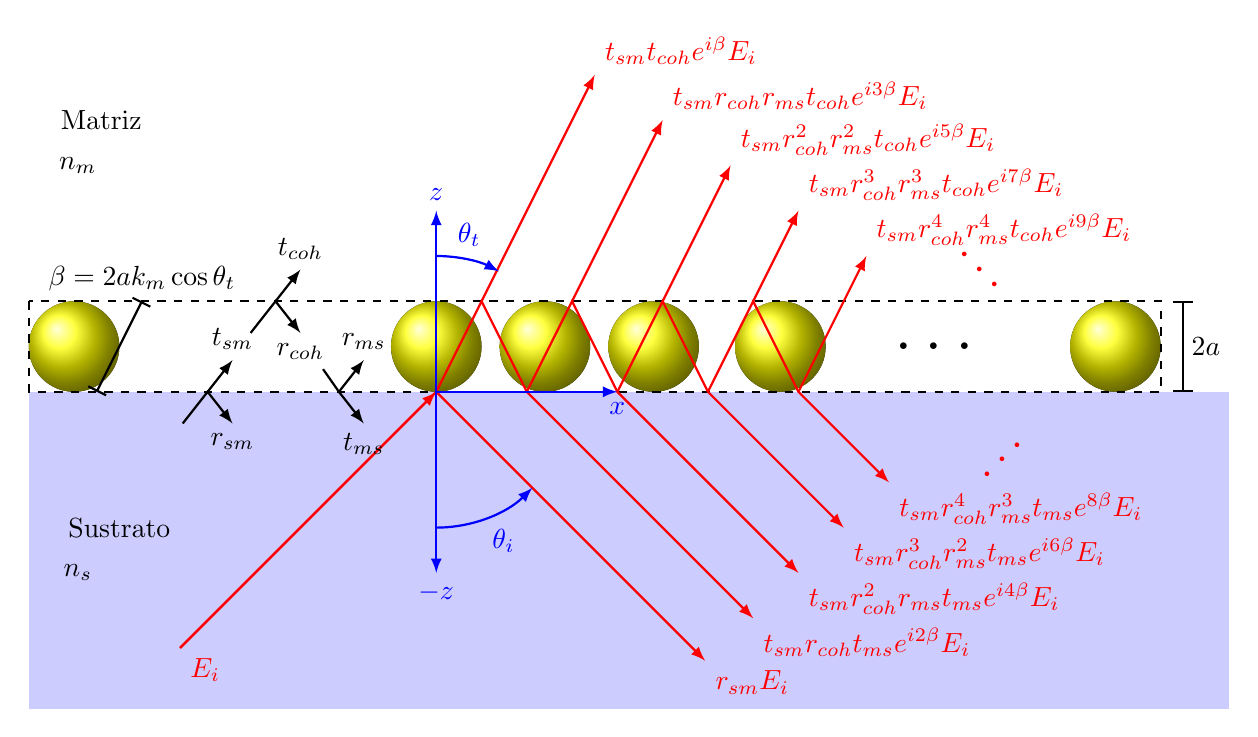
\begin{tikzpicture}[scale=1.15]
\def\a{.5}
\def\d{.5}
\def\t{.3}

\fill[blue, opacity = .2] (-4.5,-3.5) rectangle(8.75,0);

\foreach \x in {-4,0,1.2,2.4,3.8,7.5}{ %-2.9,-1.1
\fill[ball color=yellow, opacity=1] (\x,\d) circle(\a);}

\draw[thick, dashed] (-4.5,2*\d) rectangle (8,0);
\node at (5.5,\d) {\Huge $\ldots$};


%%%%%%%%%%%%%-------------Reflexiones
%
%\draw[latex -, thick, red](-135:0)--(-135:4) node[anchor=north]{$E_i$};
%\draw[- latex, thick, red](-135:4)--(-135:0)--(-45:4) node[anchor=north]{$r_{coh}E_i$};
%\draw[- latex, thick, red](0,0)--(2*\d,2*\d)--(3+2*\d,-3+2*\d) node[anchor=south west]{$t_{coh}r_{ms}t_{coh}E_i$};
%\draw[- latex, thick, red](4*\d,0)--(6*\d,2*\d)--(3+6*\d,-3+2*\d) node[anchor=south west]{$r_{coh}E_i$};


\draw[latex -, thick, red](-135:0)--(-135:4) node[anchor=north west]{$E_i$};
\draw[- latex, thick, red](-135:4)--(-135:0)--(-45:4.2) node[anchor=north west]{$r_{sm}E_i$};
\draw[- latex, thick, red](0,0)--(1*\d,2*\d)--(2*\d,0)--(3+\d,-3+\d) node[anchor=north west]{$t_{sm}r_{coh}t_{ms}e^{i2\beta}E_i$};
\draw[- latex, thick, red](2*\d,0)--(3*\d,2*\d)--(4*\d,0)--(3+2*\d,-3+2*\d) node[anchor=north west]{$t_{sm}r_{coh}^2r_{ms}t_{ms}e^{i4\beta}E_i$};
\draw[- latex, thick, red](4*\d,0)--(5*\d,2*\d)--(6*\d,0)--(3+3*\d,-3+3*\d) node[anchor=north west]{$t_{sm}r_{coh}^3r_{ms}^2t_{ms}e^{i6\beta}E_i$};
\draw[- latex, thick, red](6*\d,0)--(7*\d,2*\d)--(8*\d,0)--(3+4*\d,-3+4*\d) node[anchor=north west]{$t_{sm}r_{coh}^4r_{ms}^3t_{ms}e^{8\beta}E_i$};
\draw[-, thick, red](8*\d,0)--(9*\d,2*\d);
\node[rotate={45}] at (6.25,-.75) {\color{red}\LARGE $\ldots$};

%%%%%%%%%%%%%-------------transmisiones
\draw[- latex, thick, red](1*\d,2*\d)--(1.75,3.5) node[anchor=south west]{$t_{sm}t_{coh}e^{i\beta}E_i$};
\draw[- latex, thick, red](3*\d,2*\d)--(2+1*\d,4-2*\d) node[anchor=south west]{$t_{sm}r_{coh}r_{ms}t_{coh}e^{i3\beta}E_i$};
\draw[- latex, thick, red](5*\d,2*\d)--(2+2.5*\d,4-3*\d) node[anchor=south west]{$t_{sm}r_{coh}^2r_{ms}^2t_{coh}e^{i5\beta}E_i$};
\draw[- latex, thick, red](7*\d,2*\d)--(2+4*\d,4-4*\d) node[anchor=south west]{$t_{sm}r_{coh}^3r_{ms}^3t_{coh}e^{i7\beta}E_i$};
\draw[- latex, thick, red](9*\d,2*\d)--(2+5.5*\d,4-5*\d) node[anchor=south west]{$t_{sm}r_{coh}^4r_{ms}^4t_{coh}e^{i9\beta}E_i$};
\node[rotate={-45}] at (6,1.35) {\color{red}\LARGE $\ldots$};



\node at (-4,2.5) {$\; n_m$};
\node at (-3.7,3) {Matriz};
\node at (-4,-2) {$\; n_s$};
\node at (-3.5,-1.5) {Sustrato};

%\draw[latex - , thick](-2.8,-.5)--(-3.5,.5) node[anchor=north]{$r_{sm},\,t_{sm}$};
\draw[latex - , thick, shift ={(.55,0)}](-2.8,-.35)node[anchor=north]{$r_{sm}$}--(-3.075,0)--(-3.35,-.35);
\draw[latex -,thick, shift ={(.55,0)}](-2.8,.35)node[anchor=south]{$t_{sm}$}--(-3.075,0);
\draw[latex - , thick, shift ={(2.0,0)}](-2.8,-.35)node[anchor=north]{$t_{ms}$}--(-3.075,0)--(-3.25,.25);
\draw[latex -,thick, shift ={(2.0,0)}](-2.8,.35)node[anchor=south]{$r_{ms}$}--(-3.075,0);
\draw[latex - , thick, shift ={(1.3,2*\d)}](-2.8,-.35)node[anchor=north]{$r_{coh}$}--(-3.075,0)--(-3.35,-.35);
\draw[latex -,thick, shift ={(1.3,2*\d)}](-2.8,.35)node[anchor=south]{$t_{coh}$}--(-3.075,0);

\draw[|-|,thick, shift ={(-3.75,0)}](0,0)--(1*\d,2*\d) node[anchor=south]{$\beta = 2ak_m\cos\theta_t$};

\draw[|-|,thick, shift ={(8.25,0)}](0,0)--(0,2*\d) ;
\node at (8.5,\d){$2a$};

\draw[- latex, thick, blue] (0,0)--(90:2) node[anchor = south]{$z$};
\draw[- latex, thick, blue] (0,0)--(90:-2) node[anchor = north]{$-z$};
\draw[- latex, thick, blue] (0,0)--(0:2) node[anchor = north]{$x$};
\path (0,0)++(85:1.5)node[anchor=south west, blue]{$\theta_t$}; 
\draw[- latex, thick, blue](90:1.5)arc(90:62.5:1.5);
\path (0,0)++(-70:1.5)node[anchor=north west, blue]{$\theta_i$}; 
\draw[- latex, thick, blue](-90:1.5)arc(-90:-45:1.5);


\end{tikzpicture}
	\caption{ Esquema de las múltiples reflexiones en ATR del sistema matriz-monocapa-sustrato producidos por una onda plana $\vb{E}^i$ que incide en la interfaz de un sustrato, con índice de refracción $n_s$, que sostiene a una monocapa de NPs esféricas de radio $a$ inmerza en una matriz con $n_m$, a un ángulo $\theta_i$ respecto a la dirección normal a la interfaz. Las reflexiones y transmisionees en la interfaz sustrato-matriz ($z=0$) es descrita por los coeficientes de amplitud de Fresnel [Ecs. \eqref{eq:rs}--\eqref{eq:tp}] en $\theta_i$, mientras que en la intfaz monocapa-matriz ($z=2a$) las reflexiones y transmisiones son descritsd por el CSM [Ecs. \eqref{eqs:rtcoh}] en $\theta_t$. En los coeficientes de amplitud  $r_{\alpha\beta}$ y $t_{\alpha\beta}$ el medio de incidencia del haz de luz es $\alpha$ y el de transmisión en $\beta$.}\label{fig:CSM-ATR}
	\end{figure}



	\begin{align}
	r =& r_{sm} + t_{sm}r_{coh}t_{ms}e^{2i\beta}\left[1+r_{coh}r_{ms}e^{2i\beta}+\qty(r_{coh}r_{ms}e^{2i\beta})^2+\qty(r_{coh}r_{ms}e^{2i\beta})^3+\ldots,\right] \notag \\
		=& r_{sm} + \frac{ t_{sm}r_{coh}t_{ms}e^{2i\beta}}
				{1-r_{ms}r_{coh}e^{i2\beta}}, \label{eq:r_ATR_preStokes} \\
	t =& t_{coh}t_{ms}e^{i\beta} \left[1+r_{coh}r_{ms}e^{2i\beta}+\qty(r_{coh}r_{ms}e^{2i\beta})^2+\qty(r_{coh}r_{ms}e^{2i\beta})^3+\ldots\right]
	=\frac{  t_{coh}t_{ms}e^{i\beta} }
				{1-r_{ms}r_{coh}e^{i2\beta}}.\notag
	\end{align}
%
Es posible reescribir la Ec. \eqref{eq:r_ATR_preStokes} empleando las relaciones de Stokes\footnote{Las relaciones de Stokes se deducen a partir de la invariancia de las ecuaciones de Maxwell ante inversiones temporales ($t\to -t$), y relacionan a los coeficientes de amplitud $r$ y $t$ evaluados en $\theta_i$ y $\theta_t$ para una interfaz entre medios no absorbentes. Las relaciones de Stokes son \cite{hecht1998optics,garcia2012multiple} $r_{it}(\theta_i) = -r_{ti}(\theta_t)$, $t_{it}(\theta_i) = 1+r_{it}(\theta_i)$, y $t_{ti}(\theta_t) = 1+r_{it}(\theta_t)$.}, por lo que se obtiene \begin{subequations}\vspace*{-.75em}
%
\begin{tcolorbox}[title = Coeficientes de amplitud de CSM en configuración ATR, breakable ]
	\eqhalf{r = \frac{r_{sm}(\theta_i)+r_{coh}(\theta_t)e^{i2\beta}}
					{1-r_{coh}(\theta_t)r_{sm}(\theta_i)e^{2i\beta}},
	\label{seq:rCSMATR}}
	\eqhalf{t = \frac{t_{sm}(\theta_i)t_{coh}(\theta_t)e^{i\beta}}
									{1-r_{coh}(\theta_t)r_{ms}(\theta_t)e^{2i\beta}},
	\label{seq:tCSMATR}}
	
	con $\beta = 2a k_0n_m\cos\theta_t$.
	\end{tcolorbox}\label{eqs:rtCSMATR}\end{subequations}\vspace*{-.75em}






\chapter{Resultados numéricos}

Para estudiar la respuesta electromagnética (EM) de una monocapa de nanopartículas (NPs) inmersa en un medio dieléctrico, denominado matriz, y soportada sobre un sustrato dieléctrico, se emplea el formalismo del modelo de esparcimiento coherente (Coherent Scattering Model, CSM) para calcular la reflectancia $R$ y transmistancia $T$ del sistema \cite{reyes2018analytical}. El CSM proporciona expresiones analíticas de los coeficientes de amplitud de reflexión $r$ y transmisión $t$ de la monocapa cuando está suspendida en el espacio libre (Free Stanting Monolayer, FSM) [Ecs. \eqref{eqs:rtcoh}], y para el sistema matriz-monocapa-sustrato tanto en incidencia externa [Ecs. \eqref{eqs:rtCSMext}] como interna, o bien en una configuración de reflexión total atenuada \index{Reflexión total!atenuada} (Attenuated Total Reflection, ATR) [Ecs. \eqref{eqs:rtCSMATR}]. En la primera sección de este capítulo se calcula la respuesta EM de una moncapa de NPs esféricas considerando que la función dieléctrica de las NPs que conforman la monocapa está dada por el modelo de Drude-Sommerfeld [Ec. \eqref{eq:Drude}], que depende de sólo dos parámetros: la frecuencia de plasma $\omega_p$, que sintoniza las resonancias plasmónicas de superficie (Surface Plasmon Resonances, SPRs), y la constante fenomenológica de amortiguamiento $\gamma$, que ajusta el ancho de cada SPR. En caso de identificar en el cálculo de la refectancia y transmitancia de una monocapa de NPs excitaciones distintas a las  SPRs de partículas individuales (Single Particles SPR, SP-SPRs), como el \emph{modo guiado} reportado en \cite{kabashin2009plasmonic} y \cite{danilov2018ultra}, también denominado resonancia de red de plasmón de superfice (Surface Plasmon Lattice Resonance, SPLR), la elección de $\omega_p$ y $\gamma$ evita el traslape entre ambas excitaciones y facilita la identificación de cada modo. En la segunda sección se emplean las correcciones por tamaño para partículas esféricas de las funciones dieléctricas del oro y de la plata, para identificar si un modo semejante al modo guiado se encuentra en monocapas formadas con NPs de materiales reales, así como las  características de la monocapa para que pueda ser empleada en el biosensado.

\section{Resultados con el modelo de Drude-Sommerfeld}
\label{section:Drude}


 En la primera subsección se analiza la reflectancia de una FSM empleando el modelo de Drude-Sommerfled con parámetros $\hbar\omega_p = 4.3$ eV y  $\hbar\gamma = 0.15$ eV [ver Fig. \ref{sfig:Drude4eV}], y comparando la respuesta EM de la monocapa con la de una partícula individual. En la segunda subsección se estudia la reflectancia de una monocapa soportada en configuración de reflexión interna atenuada, ver Fig. \ref{sfig:ATR}, empleando el modelo de Drude-Sommerfeld en un primer caso con los parámetros  $\hbar\omega_p = 4.3$ eV y  $\hbar\gamma = 0.15$ eV, y posteriormente con $\hbar\omega_p = 10$ eV y $\hbar\gamma = 0.15$ eV [ver Fig. \ref{sfig:Drude10eV}] para modificar la longitud de onda de las SP-SPRs; ulteriormente se calcula la reflectancia de la monocapa considerando  variaciones en la fracción de cubierta $\Theta$ y el radio $a$ de las NPs, parámetros que modifican las proporciones del sistema, tales como la distancia promedio entre las NPs, y la cantidad de electrones libres sobre la monocapa. Adicional al cálculo de la reflectancia, se calculó la transmitancia de la monocapa para las dos funciones dieléctricas, con $\hbar\omega_p =4.3$ eV y $\hbar\omega_p =10$ eV, para corroborar que los modos distintos a las SP-SPRs tienen un comportamiento semejante a un modo guiado. 
	
	\subsection{Reflectancia de una monocapa suspendida en aire}
	\label{ssection:DrudeFSM}
	
	
Para el cálculo de la reflectancia mediante el CSM de una FSM suspendida en una matriz con $n_m=1.33$, modelando al agua en el espectro visible \cite{INDREF}. Se empleó la Ec.  \eqref{eq:R} con el coeficiente de amplitud de reflexión coherente $r_{coh}$ [Ec.  \eqref{seq:rcoh}].  En la Fig.  \ref{fig:R-FSM} se muestran los resultados de la reflectancia $R$ en función del ángulo de incidencia $\theta_i$ y tanto de la longitud de onda $\lambda$ del haz incidente (escala inferior), como de la energía del haz incidente en unidades de $\hbar\omega = h c /\lambda$ (escala superior).  La frecuencia de plasma empleada para la función dieléctrica tipo Drude fue $\hbar\omega_p = 4. 3$ eV y la constante fenomenológica de amortiguamiento $\hbar\gamma = 0. 15$ eV (que corresponden a $288. 5$ nm  y $8,270$ nm, respectivamente). Se consideraron NPs de radio $a=30$ nm y fracciones de cubierta $\Theta$: $0. 05$, $0. 1$, $0. 2$, $0. 3$ y $0. 4$. En el renglón superior de la Fig. \ref{fig:R-FSM}, gráficas de $\mathbf{i)}$ a $\mathbf{v)}$, se muestra la reflectancia para polarización \emph{p}, mientras que en el renglón inferior se presentan las gráficas para polarización \emph{s}, $\mathbf{vi)}$ -- $\mathbf{x)}$. La línea punteada vertical verde  en $\lambda \approx 658$ nm corresponde a la SP-SPR dipolar ($\ell = 1$), mientras que la línea vertical rosa punteada en $\lambda \approx 561$ nm corresponde a la excitación del modo cuadrupolar ($\ell=2$).
					
	\begin{figure}[h!]\centering
	\begin{tikzpicture}
\node[inner sep=0pt] (graf) at (-.15,0){\includegraphics[width = .9\linewidth]{2-Resultados/figs/4-Wp4FSMThetaVar/0-2D_Grid.png}};
\node[right, inner sep=0pt] (legend) at (7,.1) {\includegraphics[scale=.77, trim={00 00 00 00}, clip]{2-Resultados/figs/0-IBar_v}};
\node[above, inner sep=0pt] (r) at (7.15,3.2) {$R$};
\end{tikzpicture}\vspace*{-.5em}
	\caption{Gráficas de la reflectancia para una FSM como función del ángulo de incidencia $\theta_i$ y tanto de la longitud de onda $\lambda$ (escala inferior), como de la energía del haz incidente en unidades de $\hbar\omega$ (escala superior), para una función dieléctrica tipo Drude con $\hbar\omega_p=4. 3$ eV  y  $\hbar\gamma=0. 15$ eV.  Las gráficas   en el renglón superior [$\mathbf{i)-v)}$]  muestran los resultados de reflectancia para  polarización \emph{p} y las del renglón inferior  [$\mathbf{i)-v)}$] para polarización  \emph{s}, donde se consideraron NPs de radio $a=30$ nm y distintas fracciones de cubierta $\Theta$: $0. 05$, $0. 1$, $0. 2$, $0. 3$ y $0. 4$. Las líneas verticales punteadas verdes y rosas corresponden a las SP-SPRs dipolar ($658$ nm) y cuadrupolar ($561$ nm), respectivamente.}	\label{fig:R-FSM}	
	\end{figure}		
					
La reflectancia para polarización \emph{p} [Fig. \ref{fig:R-FSM} $\mathbf{i)-v)}$] es cero para el ángulo de Brewster $\theta_B = 45^\circ$ y para regiones alejadas de las SP-SPRs (líneas punteadas verticales verde y rosa  localizadas en $658$ nm y $561$ nm, respectivamente). En la gráfica \textbf{v)}, $\Theta=0.4$,  se observa a $561$ nm (escala inferior) y $\theta_i>50^\circ$ que $R\approx 0$ sin embargo, la reflectancia aumenta para longitudes de onda mayores y menores a $658$ nm. Conforme la fracción de cubierta disminuye, gráficas \textbf{iii)} y \textbf{iv)}, la extinción de luz a $561$ nm  es menos evidente y para las fracciones de cubierta $\Theta=0.1$ y $0.05$, gráficas \textbf{ii)} y \textbf{i)}, ya no es apreciable la extinción de luz a la frecuencia de la SP-SPR dipolar. En contraparte, para polarización \emph{s} [Fig. \ref{fig:R-FSM} $\mathbf{vi)-x)}$] la reflectancia es apreciable para todo ángulo de incidencia a las frecuencias de las SP-SPRs. 

Para comparar la respuesta EM  de una FSM al variar la fracción de cubierta, se grafican en la  Fig. \ref{fig:FSM-Cuts} cortes de la reflectancia para $\theta_i = 65^\circ$, ángulo en donde se extingue la luz reflejada al rededor de la SP-SPR dipolar para fracciones de cubierta $\Theta>0.2$ en la Fig. \ref{fig:R-FSM}. Se muestran cortes de la reflectancia tanto para un haz incidente con polarización \emph{p} $R_p$ [Fig. \ref{sfig:FSM-cutp}], como uno con polarización \emph{s} $R_s$ [Fig. \ref{sfig:FSM-cuts}]. Para la polarización \emph{p} se presenta un mínimo en la reflectancia alrededor de $658$ nm para fracciones de cubierta mayores a $\Theta = 0.05$. Los mínimos de $R_p$ a la frecuencia de la SP-SPR dipolar son más pronunciados conforme aumenta la fracción de cubierta sin embargo, para $\Theta=0.05$ se observa un máximo en lugar de un mínimo. Para polarización \emph{s}, se presenta un máximo en la reflectancia a $658$ nm para todos los valores de $\Theta$. Para las fracciones de cubierta mayores, $\Theta = 0.3$ y $\Theta = 0.4$,  se observa un  mínimo en la reflectancia alrededor de $561$ nm para ambas polarizaciones, lo que corresponde a la SP-SPR cuadrupolar.

		\begin{figure}[h!]\centering\hspace*{-1.5em}
	\begin{subfigure}{.01\linewidth}\caption{}\label{sfig:FSM-cutp}\vspace{4.5cm}\end{subfigure}
	\begin{subfigure}{.45\linewidth}\hspace*{-1.5em}
	\includegraphics[scale=1]{2-Resultados/figs/4-Wp4FSMThetaVar/cut_angle_65_p.pdf}\end{subfigure}
	\begin{subfigure}{.01\linewidth}\caption{}\label{sfig:FSM-cuts}\vspace{4.5cm}\end{subfigure}\hspace*{-1.em}
	\begin{subfigure}{.45\linewidth}\centering
	\includegraphics[scale=1 ]{2-Resultados/figs/4-Wp4FSMThetaVar/cut_angle_65_s.pdf}\end{subfigure}\vspace*{-.5em}
	\caption{Cortes de la Fig. \ref{fig:R-FSM} a $\theta_i = 65^\circ$ de reflectancia de una FSM de NPs esféricas de radio $a=30$ nm en polarización \textbf{a)} \emph{p} y \textbf{b)} \emph{s} como función tanto de la longitud de onda $\lambda$ (escala inferior), como de la energía del haz incidente en unidades de $\hbar\omega$ (escala superior). Los parámetros de la función dieléctrica tipo Drude para las NPs son $\hbar\omega_p = 4.3$ eV y $\hbar\gamma = 0.15$ eV y las fracciones de cubierta consideradas fueron $\Theta$: $0. 05$, $0. 1$, $0. 2$, $0. 3$ y $0. 4$. Las líneas verticales punteadas verdes y rosas corresponden a las SP-SPRs dipolar ($658$ nm) y cuadrupolar ($561$ nm), respectivamente.}\label{fig:FSM-Cuts}
	\end{figure}	

Al calcular la distancia mínima promedio $\langle d_{min}\rangle$ entre las NPs  de $a = 30$ nm mediante la Tab. \eqref{tab:MeanD}, se obtiene que $\langle d_{min} \rangle = 177.8$ nm para $\Theta = 0.05$. El análisis de una partícula individual es válido para el caso de $\Theta=0.05$ (en negro en la Fig. \ref{fig:FSM-Cuts}), debido a la distancia promedio entre las NPs, por tanto, la presencia del máximo en la reflectancia en la SP-SPRs dipolar (línea punteada vertical verde) corresponde a una cota mínima en $R_p$ debido al esparcimiento de cada una de las NPs; como se observa en las gráficas de las eficiencias de extinción y de esparcimiento graficadas en la Fig. \ref{fig:QextDrude}.

En las Figs. \ref{fig:R-FSM} y \ref{fig:FSM-Cuts} se observa la respuesta EM de una monocapa de NPs suspendida en un medio con $n_m=1.5$ al interactuar con una onda plana. Si se considera la presencia de un sustrato que soporte la monocapa, se puede estar en configuraci\'on de incidencia externa o interna, seg\'un sea el medio de incidencia de la onda plana. Para incidencia externa, a todo ángulo de incidencia,  una onda plana ilumina a las NPs de la monocapa por lo que, respecto al caso de la FSM, la posición de los máximos y mínimos de la reflectancia no cambiarán y los valores de $R$ presentarán un decrecimiento, debido al sustrato que disminuye el contraste entre índice de refracción de las NPs en la monocapa y el medio de transmisión. Por otro lado, para el caso de incidencia interna y ángulos mayores al ángulo crítico $\theta_c = \arcsin(n_m/n_s)$, las NPs en la monocapa son iluminadas por ondas evanescentes, por tratarse de un configuración en ATR, por lo que es posible  observar cambios en la respuesta EM de la monocapa, como sucede  cuando se tiene una placa continua y se excitan plasmones polaritones de superficie.

	\subsection{Reflectancia y transmitancia de una monocapa soportada sobre un sustrato en configuración de reflexión total atenuada}
	\label{ssection:DrudeATR}

La respuesta EM de una monocapa de NPs, suspendida en una matriz con índice de refracción $n_m$ y soportada por un sustrato con índice de refracción $n_s$, se calcula al emplear la Ec.  \eqref{eq:R} con el coeficiente de amplitud de reflexión $r$ de la Ec.  \eqref{seq:rCSMATR}. Para comparar los resultados de la reflectancia $R$ para una FSM y una monocapa en configuración ATR, se emplean los parámetros utilizado en los cálculos de las Figs. \ref{fig:R-FSM} y \ref{fig:FSM-Cuts} ($n_m=1.33$ , $a=30$ nm, $\hbar\omega_p=4.3$ eV y  $\hbar\gamma = 0.15$ eV) considerando un sustrato con índice de refracción $n_s=1.5$, pues el índice de refracción del vidrio BK7 es $n_{BK7}=1.50\pm 0.05$ en un intervalo de longitud de onda entre $334.1$ nm y $2,325.4$ nm \cite{schott2019datasheet}. En la Fig.  \ref{fig:R-ATR4} se presentan los resultados de la reflectancia $R$ en función del ángulo de incidencia $\theta_i$ y tanto de la longitud de onda $\lambda$ del haz incidente (escala inferior) como de la energía del haz $\hbar\omega$ (escala superior). Las gráficas \textbf{i) -- v}) en la Fig. \ref{fig:R-ATR4}  corresponden a la polarización \emph{p}, mientras que las gráficas \textbf{vi) -- x)} a polarización \emph{s}. Al igual que para la FSM, se consideraron los casos para la fracción de cubierta $\Theta = 0.05,\,0.1,\,0.2,\,0.3$ y $0.4$. Las SP-SPRs corresponden a la línea vertical verde punteada en $\lambda \approx 658$ nm para el modo dipolar y la línea vertical rosa punteada en  $\lambda \approx 561$ nm para el modo cuadrupolar. Adicionalmente, los puntos amarillos en la Fig. \ref{fig:R-ATR4} corresponden a los mínimos en $R$ para ángulos mayores al ángulo crítico entre el sustrato y la matriz ($\theta_c\approx 62.5^\circ$) y longitudes de onda mayores a la SP-SPR dipolar.

	\begin{figure}[h!]\centering
\begin{tikzpicture}
\node[inner sep=0pt] (graf) at (-.1,0){\includegraphics[width = .9\linewidth]{2-Resultados/figs/1-Wp4ThetaVar/0-2D_Grid}};
\node[right, inner sep=0pt] (legend) at (7,.05) {\includegraphics[scale=.77, trim={00 00 00 00}, clip]{2-Resultados/figs/0-IBar_v}};
\node[above, inner sep=0pt] (r) at (7.15,3.2) {$R$};
\end{tikzpicture}\vspace*{-.5em}
	\caption{Gráficas de la reflectancia de una monocapa en configuración ATR como función del ángulo de incidencia $\theta_i$ y de la longitud de onda $\lambda$ (escala inferior) así como de la energía del haz incidente en unidades de $\hbar\omega$ (escala superior), para una función dieléctrica tipo Drude con $\hbar\omega_p=4. 3$ eV  y  $\hbar\gamma=0. 15$ eV.  Las gráficas   en el renglón superior [$\mathbf{i)-v)}$]  muestran los resultados de reflectancia para  polarización \emph{p} y las del renglón inferior  [$\mathbf{vi)-x)}$] para polarización  \emph{s}, donde se consideraron NPs de radio $a=30$ nm y distintas fracciones de cubierta $\Theta$: $0. 05$, $0. 1$, $0. 2$, $0. 3$ y $0. 4$. Las líneas verticales punteadas verdes y rosas corresponden a las SP-SPRs dipolar ($658$ nm) y cuadrupolar ($561$ nm), respectivamente.	os puntos amarillos corresponden a los mínimos en $R$ para ángulos mayores a $\theta_c\approx 62.5^\circ$ y longitudes de onda mayores a la SP-SPRs dipolar.}	\label{fig:R-ATR4}	
	\end{figure}	

En la Fig.  \ref{fig:R-ATR4} se observa que $R\approx 1$ para ángulos mayores al ángulo crítico, $\theta_c \approx 62.5^\circ $ excepto en dos regiones: a las longitudes de onda correspondientes a las SP-SPRs (líneas punteadas verticales) y en una región a longitudes de onda mayores a la SP-SPR dipolar (puntos amarillos). La disminución en la reflectancia después del ángulo crítico alrededor de la SP-SPR cuadrupolar ($561$ nm) es resultado de la extinción de luz debido a la presencia de las NPs y es apreciable tanto para polarización \emph{p} como para \emph{s}, siendo más evidente para las fracciones de cubierta consideradas mayores. Por ejemplo, en el panel superior de la Fig. \ref{fig:R-ATR4},  la excitación cuadrupolar de una sola partícula es apreciable en $\lambda \approx 658$ nm cuando $R_p$ disminuye para $\Theta = 0.4$, gráfica  $\mathbf{v)}$, en comparación a $\Theta = 0.05$, $\mathbf{i)}$. A pesar de que este comportamiento es análogo para la polarización \emph{s}, panel inferior de la  Fig. \ref{fig:R-ATR4}, los valores de $R_s$ a las frecuencias de las SP-SPRs son mayores que los de $R_p$, como se observa al comparar las gráficas de los cálculos con $\Theta=0.3$: \textbf{iv)} para $R_p$ y \textbf{ix)} para $R_s$.

La respuesta óptica de la monocapa a $658$ nm es distinto para cada polarización. Mientras que en polarización \emph{p}, gráficas \textbf{i)}-\textbf{v)}, la SP-SPR dipolar se aprecia para todos los valores de $\Theta$ escogidos, para polarización \emph{s}, gráficas \textbf{vi)}-\textbf{x)}, esto sólo ocurre cuando $\Theta$ toma valores cercanos a cero. Adicional a la región cercana a las SP-SPRs, se observan mínimos en la reflectancia para ángulos de incidencia mayores al ángulo crítico y para longitudes de onda mayores a la SP-SPR dipolar, los cuales están  representados por los puntos amarillos en la Fig. \ref{fig:R-ATR4}. Dado que los puntos amarillos corresponden a una excitación que ocurre energías  menores en comparación a las SP-SPRs, ésta no puede ser plasmónica de partícula individual,  por lo que especula que se debe a una respuesta colectiva como la resonancia de red del plasmón de superficie (Plasmon Surface Lattice Resonance, PSLR) reportada en \cite{danilov2018ultra}. Al comparar las gráficas en la  Fig.  \ref{fig:R-ATR4} se observa que la posible excitación colectiva se corre al rojo  conforme aumenta la fracción de cubierta $\Theta$, o bien, que para valores de $\Theta$ cercanos a cero se comporta como la SP-SPR dipolar, comportamiento más evidente en polarización \emph{p} que en \emph{s} [ver \textbf{ii)} y \textbf{vi)} y \textbf{x)}]


\begin{figure}[h!]\centering\hspace*{-1.5em}
	\begin{subfigure}{.01\linewidth}\caption{}\label{sfig:R-ATR4-cutp}\vspace{4.5cm}\end{subfigure}
	\begin{subfigure}{.45\linewidth}\hspace*{-1.5em}
	\includegraphics[scale=1]{2-Resultados/figs/1-Wp4ThetaVar/cut_angle_75_p.pdf}\end{subfigure}
	\begin{subfigure}{.01\linewidth}\caption{}\label{sfig:R-ATR4-cuts}\vspace{4.5cm}\end{subfigure}\hspace*{-1.em}
	\begin{subfigure}{.45\linewidth}\centering
	\includegraphics[scale=1 ]{2-Resultados/figs/1-Wp4ThetaVar/cut_angle_75_s.pdf}\end{subfigure}\vspace*{-.5em}
	\caption{Cortes de la Fig. \ref{fig:R-ATR4} a $\theta_i = 75^\circ$ de reflectancia de una monocapa en configuración ATR de NPs esféricas de radio $a=30$ nm en polarización \textbf{a)} \emph{p} y \textbf{b)} \emph{s} como función de la longitud de onda $\lambda$ (escala inferior) y de la energía $\hbar\omega$ (escala superior). Los parámetros de la función dieléctrica tipo Drude para las NPs son $\hbar\omega_p = 4.3$ eV y $\hbar\gamma = 0.15$ eV y las fracciones de cubierta consideradas fueron $\Theta$: $0. 05$, $0. 1$, $0. 2$, $0. 3$ y $0. 4$. Las líneas verticales punteadas verdes y rosas corresponden a las SP-SPRs dipolar ($658$ nm) y cuadrupolar ($561$ nm), respectivamente. }\label{fig:R-ATR4-Cuts}
	\end{figure}	  

Dado que la presunta excitación colectiva presenta un mínimo en la reflectancia  al rededor de $\theta_i = 75^\circ$ para los casos de fracción de cubierta analizados en la Fig.  \ref{fig:R-ATR4}, se presentan cortes de la reflectancia a este ángulo en la Fig. \ref{fig:R-ATR4-Cuts}, en donde las líneas punteadas verticales corresponden a las longitudes de onda de las SP-SPRs (verde para la excitación dipolar y rosa para la cuadrupolar). En polarización \emph{p}, Fig. \ref{sfig:R-ATR4-cutp}, y polarización \emph{s}, la excitación de la monocapa para todos los valores de $\Theta$ alrededor de $\lambda \approx 561$ nm coincide con la SP-SPR cuadrupolar.  La reflectancia a la longitud de onda de la SP-SPR cuadrupolar disminuye conforme la fracción de cubierta crece, por lo que se relaciona con la cantidad de NPs presentes en la monocapa. De forma distinta, la excitación dipolar de partícula individual ($658$ nm) no se aprecia para todos los casos estudiados en la Fig. \ref{fig:R-ATR4-Cuts} y sólo coincide para $\Theta=0.3$ nm; para $0.2\leq \Theta$ se presenta un corrimiento al azul de la SP-SPR dipolar, mientras que para $\Theta=0.05$ (línea sólida negra) se corre al rojo, empalmándola con el presunto modo colectivo de la monocapa. El mínimo en la reflectancia a $\lambda\approx 715$ nm  se atribuye al modo colectivo y no a la SP-SPR debido a que el la reflectancia toma valores cercanos a cero, comportamiento no spreciable para los corrimientos al azul de la SP-SPR dipolar. Para el caso de polarización \emph{s}, no hay corrimientos al azul de la SP-SPR dipolar, sino sólo se aprecia el presunto modo colectivo a $\lambda>658$ nm.

Los mínimos a $\lambda>650$ nm, que corresponden al presunto modo colectivo, presentan un corrimiento al rojo conforme la fracción de cubierta de la monocapa aumenta  para ambas polarizaciones, contrario al comportamiento observado en las excitaciones dipolares de partícula individual de la monocapa observadas en la Fig. \ref{sfig:R-ATR4-cutp} entre $561$ nm y $658$ nm. Otra diferencia entre las excitaciones en $\lambda$ mayores a las SP-SPRs y los corrimientos al azul de éstas, es que la disminución en el valor de $R$ no es monótona, sino que el decrecimiento en $R$ es máximo a fracciones de cubierta medias. Por lo anterior, los mínimos en $R_p$ y $R_s$ localizados a longitudes de onda mayores a la de los modos plasmónicos de partícula individual no son corrimientos de las excitaciones multipolares de una partícula, sino una probable respuesta colectiva de las NPs en la monocapa. El corrimiento al rojo del modo colectivo es mayor para  polarización \emph{p} que para \emph{s}, como se observa para $\Theta=0.1$ (línea naranja sólida), en donde al mínimo en $R$ se localiza a $765$ nm para \emph{p} y  a $740$ nm para \emph{s}.

\begin{figure}[t!]\centering
\begin{tikzpicture}
\node[inner sep=0pt] (graf) at (-.1,0){\includegraphics[width = .9\linewidth]{2-Resultados/figs/2-Wp10ThetaVar/0-2D_Grid}};
\node[right, inner sep=0pt] (legend) at (7,.05) {\includegraphics[scale=.77, trim={00 00 00 00}, clip]{2-Resultados/figs/0-IBar_v}};
\node[above, inner sep=0pt] (r) at (7.15,3.2) {$R$};
\end{tikzpicture}\vspace*{-.5em}
	\caption{Gráficas de la reflectancia de una monocapa en configuración ATR como función del ángulo de incidencia $\theta_i$ y de la longitud de onda $\lambda$ (escala inferior), así como de la energía del haz incidente en unidades de $\hbar\omega$ (escala superior), para una función dieléctrica tipo Drude con $\hbar\omega_p=10$ eV  y  $\hbar\gamma=0. 15$ eV.  Las gráficas   en el renglón superior [$\mathbf{i)-v)}$] muestran los resultados  para  polarización \emph{p} y las del renglón inferior  [$\mathbf{vi)-x)}$] para polarización  \emph{s}, donde se consideraron NPs de radio $a=30$ nm y distintas fracciones de cubierta $\Theta$: $0. 05$, $0. 1$, $0. 2$, $0. 3$ y $0. 4$. Las líneas verticales punteadas verdes, rosas y cianes corresponden a las SP-SPRs dipolar ($342$ nm), cuadrupolar ($262$ nm) y octopolar ($195$ nm), respectivamente.  Los puntos amarillos corresponden a los mínimos en $R$ para ángulos mayores a $\theta_c\approx 62.5^\circ$ y longitudes de onda mayores a la SP-SPRs dipolar. }	\label{fig:R-ATR10}	
	\end{figure}	
	
Para $\Theta = 0.3$ y $0.4$, el presunto modo colectivo se separa de la SP-SPRs dipolar (línea punteada vertical verde) a longitudes mayores a $900$ nm, por lo que 
no son apreciables en la Fig. \ref{fig:R-ATR4-Cuts}. Sin embargo, al escoger valores de $\Theta$ entre $0.05$ y $0.2$, es posible sintonizar la resonancia del presunto modo colectivo entre $715$ nm y $890$ nm para polarización \emph{p}, o bien, entre $715$ y $815$ para polarización \emph{s}. Si el presunto modo colectivo depende no sólo de la fracción de cubierta de la monocapa, sino también del material de las NPs, su posición cambiará al incrementar la frecuencia de plasma en el modelo de Drude, que caracteriza la respuesta EM de las NPs y modifica la posición de las SP-SPRs: al considerar $\hbar\omega_p = 10$ eV las SP-SPRs se corren al azul. Los resultados de la reflectancia de un sistema monocapa con los parámetros empleados en la Fig. \ref{fig:R-ATR4}, pero con $\hbar\omega_p = 10$ eV, se muestran en la Fig. \ref{fig:R-ATR10}. Las líneas verticales punteadas verde y rosa en $342$ nm y $262$ nm corresponden a las SP-SPRs dipolar y cuadrupolar,respectivamente, mientras que los puntos amarillos corresponden al presunto modo colectivo .
				
	
En las gráficas mostradas en la Fig. \ref{fig:R-ATR10} ($\hbar\omega_p = 10$ eV) se aprecian características semejantes a las observadas en la Fig. \ref{fig:R-ATR4} donde se empleó $\hbar\omega_p = 4.3$ eV. La excitación de la SP-SPR dipolar (líneas verticales punteadas rosas) sólo es apreciable para polarización \emph{p} y para $\Theta = 0.05$ para polarización  \emph{s}. Para ambas polarizaciones la reflectancia disminuye para $\theta_i>\theta_c=62.5^\circ$ y valores de $\lambda$ cercanos a la SP-SPR cuadrupolar (líneas verticales punteadas rosas), así como en longitudes de onda mayoes a la SP-SPR dipolar, es decir, en la presunta excitación colectiva  (puntos amarillos); de igual forma, el corrimeinto al rojo de la presunta excitación colectiva respecto a la SP-SPR dipolar es mayor para polarización \emph{p} que para \emph{s}.  Asimismo, al modificar el parámetro $\hbar\omega_p$ de $4.3$ eV a $10$ eV se sintonizó la presunta excitación colectiva a longitudes de onda menores, por ejemplo, para $\Theta = 0.3$, para todo ángulo de incidencia $\theta_i$, la presunta excitación colectiva se encuentra a $\lambda<900$ nm para $\hbar\omega_p=10$ eV, mientras que para $\hbar\gamma=4.3$ eV el modo colectivo ya no se apreciaba en el espectro visible, como se puede observar en las gráficas \textbf{iv)} y \textbf{ix)} de las Figs. \ref{fig:R-ATR4} y \ref{fig:R-ATR10}.

Dado que la elección del parámetro $\omega_p$ sintoniza tanto las SP-SPRs como el presunto modo colectivo, la separación entre estos puede modificarse. Para comparar con el caso de $\hbar\omega_p=4.3$ eV [Fig. \ref{fig:R-ATR4-Cuts}], se grafica en la Fig. \ref{fig:R-ATR10-Cuts} cortes de la reflectancia graficada en la Fig. \ref{fig:R-ATR10}, donde se emplea $\hbar\omega_p = 10$ eV, a $\theta_i = 75^\circ$ para ambas polarizaciones,  Fig. \ref{sfig:R-ATR10-cutp} para \emph{p} y Fig. \ref{sfig:R-ATR10-cuts} para \emph{s}, en  función de la longitud de onda, para una monocapa de NPs de radio $a= 30$ nm  y fracciones de cubierta consideradas en la Fig. \ref{fig:R-ATR10}; las líneas punteadas verde y rosa  corresponden a las SP-SPRs dipolar y cuadrupolar, respectivamente. Para ambas polarizaciones y para todas las fracciones de cubierta, se presenta una excitación a la longitud de onda correspondiente a la SP-SPR octopolar $\lambda=240$ nm, la cual se corre al azul para polarización \emph{p} pero no para \emph{s}, al igual que  la SP-SPR cuadrupolar al rededor de $262$ nm (línea punteada vertical rosa). De forma semejante a la elección del parámetro $\hbar\omega_p = 4.3$ eV, para $\hbar\omega_p=10$ eV la reflectancia de la monocapa a $\theta_i=75^\circ$ (Fig. \ref{fig:R-ATR4-Cuts}) para $0.2\leq\Theta$, se presenta un corrimiento al azil de la SP-SPR dipolar (línea punteada vertical verde). Para $\Theta=0.05$ y $0.1$, también para polarización \emph{p}, al igual que para todos los valores de $\Theta$ para \emph{s}, no se distingue la SP-SPR dipolar, sino que se presenta el presunto modo colectivo a longitudes de onda mayores a $342$ nm.

\begin{figure}[h!]\centering\hspace*{-1.5em}
	\begin{subfigure}{.01\linewidth}\caption{}\label{sfig:R-ATR10-cutp}\vspace{4.5cm}\end{subfigure}
	\begin{subfigure}{.45\linewidth}\hspace*{-1.5em}
	\includegraphics[scale=1]{2-Resultados/figs/2-Wp10ThetaVar/cut_angle_75_p.pdf}\end{subfigure}
	\begin{subfigure}{.01\linewidth}\caption{}\label{sfig:R-ATR10-cuts}\vspace{4.5cm}\end{subfigure}\hspace*{-1.em}
	\begin{subfigure}{.45\linewidth}\centering
	\includegraphics[scale=1 ]{2-Resultados/figs/2-Wp10ThetaVar/cut_angle_75_s.pdf}\end{subfigure}\vspace*{-.5em}
	\caption{Cortes de la Fig. \ref{fig:R-ATR10} a $\theta_i = 75^\circ$ de reflectancia de una monocapa en configuración ATR de NPs esféricas de radio $a$ en polarización \textbf{a)} \emph{p} y \textbf{b)} \emph{s} como función de la longitud de onda $\lambda$ (escala inferior) y de la energía en unidades de $\hbar\omega$ (escala superior). Los parámetros de la función dieléctrica tipo Drude para las NPs son $\hbar\omega_p = 10$ eV y $\hbar\gamma = 0.15$ eV y las fracciones de cubierta consideradas fueron $\Theta$: $0. 05$, $0. 1$, $0. 2$, $0. 3$ y $0. 4$. Las líneas verticales punteadas verdes, rosas y cianes corresponden a las SP-SPRs dipolar ($342$ nm), cuadrupolar ($262$ nm) y octopolar ($195$ nm), respectivamente.  }\label{fig:R-ATR10-Cuts}
	\end{figure}	

Los mínimos en la reflectancia en $\lambda > 342$ nm se atribuyen a una respuesta colectiva. Las excitaciones del presunto modo colectivo con $\hbar\omega_p = 10$ eV se comportan de manera análoga al caso de $\hbar\omega_p = 4.3$ eV: se corren al rojo conforme aumenta la fracción de cubierta y su presencia es más evidente para fracciones de cubierta media, siendo  $\Theta=0.2$ cuando la reflectancia en la excitación del presunto modo colectivo alcanza el valor mínimo de reflectancia. Cuando $\Theta = 0.05$ (líneas negras en la Fig. \ref{fig:R-ATR10-Cuts}) la excitación del presunto modo colectivo se separa de la SP-SPR dipolar   $40$ nm para ambas polarizaciones mientras que para $\Theta = 0.2$ la excitación del presunto modo colectivo se separa de la SP-SPR dipolar  $120$ nm y $100$ nm para polarización \emph{p} y \emph{s}, respectivamente, es decir, que la separación entre ambas excitaciones es menor que cuando se consideró $\hbar\omega_p = 4.3$ eV en la Fig. \ref{fig:R-ATR4-Cuts} (en donde para $\Theta=0.2$ la presunta excitación colectiva se separó de la SP-SPR dipolar más de $240$ nm). Sin embargo, la anchura a media altura (Full Width at Half Maximum, FWHM) $\Delta\lambda_{FWHM}$ de la presunta excitación colectiva es mayor para $\hbar\omega_p=10$ eV en comparación a $\hbar\omega_p=4.3$ eV. Por ejemplo, para $\Theta = 0.05$ y $\hbar\omega_p = 4.3$ eV,  $\Delta\lambda_{FWHM}\approx 200$ nm para polarización \emph{p} y  $\Delta\lambda_{FWHM}\approx 100$ nm para  \emph{s} (ver Fig. \ref{fig:R-ATR4-Cuts}), mientras que para  $\hbar\omega_p = 10$ eV,  $\Delta\lambda_{FWHM}\approx 300$ nm para polarización \emph{p} y  $\Delta\lambda_{FWHM}\approx 130$ nm para  \emph{s} (ver Fig. \ref{fig:R-ATR10-Cuts}).

%Para polarización \emph{p}, adicional a las SP-SPRs de orden $\ell = 2,\,3$ y $4$ se observa una excitación que se localiza en la longitud de onda de la SP-SPR octopolar para $\Theta=0.05$ y se corre al azul conforme aumenta la fracción de cubierta, hasta localizarse en $\lambda= 135$ nm para $\Theta=0.4$ [ver línea vertical punteada azul en laFig. \ref{sfig:R-ATR10-cutp}]. La excitación a $\lambda<185$ en polarización \emph{p} tomo un valor mínimo en la reflectancia cuando $\Theta=0.2$, una fracción de cubierta media. Esta excitación corresponde a la ramificación también presente en las gráficas \textbf{iii)} a \textbf{v)} de la Fig. \ref{fig:R-ATR10}. Ya que se observó una segunda respuesta que no corresponde a las SP-SPRs, sino que sigue las tendencias del presunto modo colectivo, se especula que es un complemento  de ellas, dado que las  PSLRs reportadas en \cite{danilov2018ultra} son, para un sistema determinado, dos excitaciones que se corren al rojo y al azul. Es decir, que tanto el modo que se corre al azul a $\lambda<185$ nm [línea punteada azul en la Fig. \ref{sfig:R-ATR10-cutp}], como el presunto modo colectivo (puntos amarilos en la Fig. \ref{fig:R-ATR10}) se pueden relacionar con las PSLRs.  

 Ya que el presunto modo colectivo sufre un corrimiento al rojo al aumentar la fracción de cubierta, se analizó si el comportamiento es semejante a cambios en el radio $a$ de las NPs.  Este análisis se llevó a cabo dado que tanto el radio $a$ como la fracción de cubierta $\Theta$ modifican el volumen neto de material plasmónico, es decir, la cantidad de electrones libres en la monocapa aumenta, así como la distancia mínima promedio $\langle d_{min}  \rangle$ entre las NPs. Si  los mínimos en $R$  a energías menores que la de la SP-SPR dipolar son sensibles al radio de las NPs, como lo son con la fracción de cubierta, se corrobora que esta excitación se debe a un efecto colectivo de las NPs.
 
Los resultados de la reflectancia de una monocapa con $\Theta=0.3$, inmersa en un medio con índice de refracción $n_m = 1.5$ y soportada por un sustrato con índice de refracción $n_m= 1.5$, se muestran en la Fig.  \ref{fig:R-RVar}, como función del ángulo de incidencia, tanto de la longitud de onda $\lambda$ (escala inferior) como de la  energía $\hbar\omega$ (escala superior) del haz incidente. Se consideraron NPs  con una respuesta EM dada dada por una función dieléctrica  tipo Drude [Ec. \eqref{eq:Drude}] con los parámetros $\hbar\omega_p =4.3$ eV y $\hbar\gamma=0.15$ eV, cuyos radios $a$ fueran los siguientes: $3$ nm, $5$ nm, $10$ nm y $20$ nm. La reflectancia en polarización \emph{p} se presenta en las gráficas $\mathbf{i)-iv)}$,mientras que en \emph{s}, en las gráficas $\mathbf{v)-viii)}$. Las SP-SPRs dipolar y cuadrupolar corresponden a las líneas punteadas verde y rosa, respectivamente. Para $a = 3$ nm y $5$ nm la excitación dipolar se localiza en $\lambda\approx 615$ nm, para el radio  $a = 10$ nm en $\lambda\approx 620$ nm y $a=20$ nm en $\lambda\approx 635$ nm, mientras que la SP-SPR cuadrupolar se localiza en $551$ nm para $a\leq 10$ nm y para el caso  $a=20$ nm, $\lambda = 555$ nm.

	\begin{figure}[h!]\centering
\begin{tikzpicture}
\node[inner sep=0pt] (graf) at (0,0){\includegraphics[width = .76\linewidth]{2-Resultados/figs/3-Wp4rVar/0-2D_Grid}};
\node[right, inner sep=0pt] (legend) at (6,.05) {\includegraphics[scale=.8, trim={00 00 00 00}, clip]{2-Resultados/figs/0-IBar_v}};
\node[above, inner sep=0pt] (r) at (6.2,3.2) {$R$};
\end{tikzpicture}\vspace*{-.5em}
	\caption{Gráficas de la reflectancia de una monocapa en configuración ATR como función del ángulo de incidencia $\theta_i$ y de la longitud de onda $\lambda$ (escala inferior), así como de la energía del haz incidente en unidades de $\hbar\omega$ (escala superior), para una función dieléctrica tipo Drude con $\hbar\omega_p=4.3$ eV  y  $\hbar\gamma=0. 15$ eV.  Las gráficas   en el renglón superior [$\mathbf{i)-v)}$] muestran los resultados para  polarización \emph{p} y las del renglón inferior  [$\mathbf{vi)-x)}$]  para polarización  \emph{s}, donde se consideró una fracción de cubierta $\Theta = 0.3$ y  NPs de radio  $a$: $3$ nm, $5$ nm, $10$ nm y $20$ nm.  Las líneas verticales punteadas verdes y rosas corresponden a las SP-SPRs dipolar y  cuadrupolar, respectivamente.  Los puntos amarillos corresponden a los mínimos en $R$ para ángulos mayores a $\theta_c\approx 62.5^\circ$ y longitudes de onda mayores a la SP-SPRs dipolar.
}	\label{fig:R-RVar}	
	\end{figure}	

En la Fig.   \ref{fig:R-RVar} (variación de $a$) la respuesta EM de la monocapa es análoga al de la Fig. \ref{fig:R-ATR4} (variación de $\Theta$) puesto que se presentan  dos regiones en $\theta_i>\theta_c=62.5^\circ$  donde se cumple que $R<1$: en $\lambda$ cercanas a las SP-SPRs y en longitudes de onda mayores a la excitación dipolar de una partícula. La distancia entre estas regiones aumenta al crecer el radio de las NPs, al igual que lo hacía al aumentar la fracción de cubierta, ademas de que esta distancia es mayor para polarización \emph{p}, que para \emph{s}. Asimismo, la SP-SPR dipolar sólo es apreciable para polarización \emph{p} a partir de NPs con radios mayores a $10$ nm; para \emph{s} la resonancia sólo es apreciable para ángulos menores al ángulo crítico ($\theta_c\approx 62.5^\circ$). Dado que la excitación a energías menores a las de las SP-SPRs (puntos amarillos) se modifica al aumentar el radio de las NPs, y no solo al cambiar el valor de la fracción de cubierta, esta excitación corresponde a un modo coletivo ya que responde a la cantidad neta de material plasmónico ---es decir, de electrones libres--- presentes en la monocapa. Para analizar la respuesta EM de la monocapa al aumentar el radio de las NPs, y compararla con la variación en $\Theta$ en la Fig. \ref{fig:R-ATR4},  se grafica la reflectancia a $\theta_i = 75^\circ$. 

En la Fig. \ref{fig:R-RVar-Cuts} se presentan cortes de la reflectancia graficada en la Fig. \ref{fig:R-RVar} a $\theta_i = 75^\circ$. Dado que la longitud de onda de las SP-SPRs depende del radio de las NPs, la excitación dipolar para los tamaños de partículas utilizadas corresponde a la región verde entre $615$ nm y $635$ nm, mientras que la cuadrupolar corresponde a la región rosa entre $551$ nm y $555$ nm.
 En los resultados de la reflectancia para polarización \emph{p}, graficados en la Fig. \ref{sfig:R-RVar-cutp}, la excitación cuadrupolar sólo es apreciable para $a=20$ nm, y la SP-SPR dipolar se identifica para los radios de $10$ nm y $20$ nm (líneas amarillas y verdes) como un mínimo en $R_p$ a $\lambda\approx 620$ nm. Para $a=5$ nm, la reflectancia $\lambda\approx 620$ nm no es mínima, sin embargo se presenta un cambio en la pendiente de la reflectancia a dicha longitud de onda; adicionalmente, en $690$ nm, la reflectancia para $a=5$ nm tiene un mínimo con $R_p<0.1$, el cual se atribuye al modo colectivo. Para $a=3$ nm (línea negra) no se manifiesta la SP-SPR dipolar sino únicamente el mínimo correspondiente al modo colectivo a $650$ nm. A partir del comportamiento de $R_p$ para $a=3$ nm y $a=5$ nm a $620$ nm, así como el corrimiento al azul de la excitación del modo colectivo al aumentar el radio de las NPs en la monoca, se concluye que para NPs con radios tendiendo a cero, la excitación colectiva corresponde a la de partícula individual.
 
 Para polarización \emph{s}, Fig. \ref{sfig:R-RVar-cuts}, la respuesta cuadrupolar sólo se observa para $a = 20$ nm y, como ocurrió en casos pasados, la SP-SPR dipolar no es apreciable. Los mínimos de la reflectancia dentro del rango de la SP-SPR dipolar se corren al rojo conforme crece el radio y la disminución en el valor de $R$ es mucho menor que la disminución  observada en la Fig. \ref{sfig:R-ATR4-cutp} (respuesta EM de la monocapa de NPs tipo Drude con $\hbar\omega_p = 4.3$, $a = 30$ nm y variaciones en $\Theta$) para la SP-SPR dipolar. Las excitaciones a $\lambda>620$ nm en la Fig. \ref{fig:R-RVar-Cuts} siguen las tendencias observadas en el modo colectivo, se atribuyen a éste y se corrobora que la excitación colectiva se traslapa con la SP-SPR dipolar cuando el radio de las NPs tiende a cero, también para polarización \emph{s}.
 
\begin{figure}[h!]\centering\hspace*{-1.5em}
	\begin{subfigure}{.01\linewidth}\caption{}\label{sfig:R-RVar-cutp}\vspace{4.5cm}\end{subfigure}
	\begin{subfigure}{.45\linewidth}\hspace*{-1.5em}
	\includegraphics[scale=1]{2-Resultados/figs/3-Wp4rVar/cut_angle_75_p.pdf}\end{subfigure}
	\begin{subfigure}{.01\linewidth}\caption{}\label{sfig:R-RVar-cuts}\vspace{4.5cm}\end{subfigure}\hspace*{-1.em}
	\begin{subfigure}{.45\linewidth}\centering
	\includegraphics[scale=1 ]{2-Resultados/figs/3-Wp4rVar/cut_angle_75_s.pdf}\end{subfigure}\vspace*{-.5em}
	\caption{Cortes de la Fig. \ref{fig:R-RVar} a $\theta_i = 75^\circ$ de las gráficas de reflectancia de una monocapa en configuración ATR (Fig. \ref{fig:R-RVar}) de NPs esféricas de fracción de cubierta $\Theta = 0.3$ en polarización \textbf{a)} \emph{p} y \textbf{b)} \emph{s} en función de la longitud de onda $\lambda$ (escala inferior) y de la energía $\hbar\omega$ (escala superior). Los parámetros de la función dieléctrica tipo Drude para las NPs son $\hbar\omega_p = 4.3$ eV y $\hbar\gamma = 0.15$ eV y las fracciones de cubierta consideradas fueron $a$: $3$ nm, $5$ nm, $10$ nm y $20$ nm. La SP-SPR dipolar para los tamaños de partículas utilizadas corresponde la región verde entre $500$ nm y $512$ nm, mientras que la cuadrupolar corresponde a la región rosa entre $456$ nm y $561$ nm.}\label{fig:R-RVar-Cuts}
	\end{figure}	

La respuesta óptica de la monocapa correspondiente al modo colectivo presenta, a un valor de $\theta_i$ fijo (Figs. \ref{fig:R-ATR4-Cuts}, \ref{fig:R-ATR10-Cuts} y \ref{fig:R-RVar-Cuts}), un ensanchamiento de la excitación, así como un corrimiento al rojo de ésta, al aumentar la fracción de cubierta de la monocapa o el radio de las NPs que la conforman. La excitación colectiva también se corre al rojo al aumentar el ángulo de incidencia, como se observa en las Figs. \ref{fig:R-ATR4}, \ref{fig:R-ATR10} y \ref{fig:R-RVar} y los  valores de la reflectancia, a las longitudes de onda de la excitación colectiva, es menor conforme aumenta el ángulo de incidencia, como se evidencia en los casos con $\Theta=0.3$ y $0.4$; otro efecto en la elección del ángulo de incidencia es la disminución del ancho de la resonancia al aunmentar $\theta_i$. La SP-SPR dipolar coincide con la excitación colectiva cuando los radios de la NPs de la monocapa, o su fracción de cubierta, tienden a cero y cuando los ángulo de incidencia son cercanos al ángulo crítico $\theta_c$. Asimismo, para polarización \emph{p} la SP-SPR dipolar es apreciable en la reflectancia y distinguible del modo colectivo, mientras que para \emph{s} no se aprecia la SP-SPR dipolar.  El valor de la reflectancia a las longitudes de onda de la excitación colectiva, así como su ancho, son dependientes del material de las NPs, por ejemplo, para  $a=30$ nm y a $\theta_i=75^\circ$ $\hbar\omega_p=4.3$ eV (Fig. \ref{fig:R-ATR4-Cuts}) la reflectancia toma el valor más cercano a cero en $715$ nm al escoger  $\Theta=0.05$ pero para $\hbar\omega_p=10$ eV (Fig. \ref{fig:R-ATR10-Cuts}) esto ocurre con $\Theta=0.1$ a $\lambda=440$ nm. 

 Dado que el modo colectivo estudiado se presenta a energías menores a la de las SP-SPRs, ésta no es una excitación plasmónica, de forma semejante que las PSLRs reportadas en  \cite{kabashin2009plasmonic} y \cite{danilov2018ultra}. Sin embargo, las PSLRs son una excitación colectiva que se presenta en un arreglo ordenado de nanocilindros \cite{kabashin2009plasmonic} y \cite{danilov2018ultra} que, además, cuenta con las características de un modo guiado, es decir, que la energía se propaga a través de la monocapa de nanocilindros \cite{kabashin2009plasmonic}. El modo colectivo  para sistemas desordenados de NPs esféricas idénticas (puntos amarillos en las Figs. \ref{fig:R-ATR4}, \ref{fig:R-ATR10} y \ref{fig:R-RVar}) se caracterizó mediante los mínimos en la reflectancia a las  longitudes de onda de excitación $\lambda_{exc}$, mayores a las de las SP-SPRs. Si la transmitancia $T$ de la monocapa evaluada en $\lambda_{exc}$ no es máxima, entonces el modo colectivo presenta características de un modo guiado, semejante a las PSLRs.

 En la Fig. \ref{fig:RT-Omegas} se muestran los cálculos de la reflectancia $R$, la transmitancia $T$ y la suma de éstas ($R+T$) de una monocapa de NPs inmersa en un medio con índice de refracción $n_m=1.5$ y soportada por un sustrato con índice de refracción $n_s=1.5$, en función del ángulo de incidencia $\theta_i$, así como de la longitud de onda $\lambda$ (escala inferior) y de la energía  $\hbar\omega$ (escala superior), tanto para polarización \emph{p}  [\textbf{i)}--\textbf{iii)}] como para \emph{s} [\textbf{iv)}--\textbf{vi)}]. Fueron seleccionados para $\hbar\omega_p=4.3$ eV [Fig. \ref{sfig:RT-4}] los parámetro $\Theta=0.2$ y $a=25$ nm puesto que el modo colectivo para estos valores se encuentra dentro del espectro visible para todo valor de $\theta_i$. Para $\hbar\omega_p=10$ eV los parámetros de la monocapa escogidos fueron $\Theta=0.3$ y $a=30$ nm, en donde se localizó al modo colectivo al rededor de $500$ nm y $850$ nm, a pesar de que las SP-SPR se encuentran en el ultra violeta.
 
\begin{figure}[h!]\centering
	\begin{subfigure}{.01\linewidth}\caption{}\label{sfig:RT-4}\vspace{6.5cm}\end{subfigure}
	\begin{subfigure}{.7\linewidth}\hspace*{-.5em}
	\begin{tikzpicture}
\node[inner sep=0pt] (graf) at (0.05,0){\includegraphics[width = .8\linewidth]{2-Resultados/figs/5-RT-Wp4-10/0-2D_Grid_1.png}};
\node[right, inner sep=0pt] (legend) at (4.5,0) {\includegraphics[scale=.77, trim={00 00 00 00}, clip]{2-Resultados/figs/0-IBar_v}};
\node[above, inner sep=0pt] (r) at (4.65,3.2) {\small $I/I_0$};
\end{tikzpicture}	
	\end{subfigure}\\
	\begin{subfigure}{.01\linewidth}\caption{}\label{sfig:RT-10}\vspace{6.5cm}\end{subfigure}\hspace*{-3.5em}
	\begin{subfigure}{.7\linewidth}\centering
	\begin{tikzpicture}
\node[inner sep=0pt] (graf) at (.05,0){\includegraphics[width = .8\linewidth]{2-Resultados/figs/5-RT-Wp4-10/0-2D_Grid_2.png}};
\node[right, inner sep=0pt] (legend) at (4.5,0) {\includegraphics[scale=.77, trim={00 00 00 00}, clip]{2-Resultados/figs/0-IBar_v}};
\node[above, inner sep=0pt] (r) at (4.65,3.2) {\small $I/I_0$};
\end{tikzpicture}
		\end{subfigure}\vspace*{-.5em}
	\caption{Gráficas de reflectancia $R$, transmitancia $T$ y la suma de éstas $R+T$ de una monocapa en configuración ATR como función del ángulo de incidencia $\theta_i$ y de la longitud de onda $\lambda$ (escala inferior) así como de la energía del haz incidente en unidades de $\hbar\omega$ (escala superior), para una función dieléctrica tipo Drude con \textbf{a)} $\hbar\omega_p=4. 3$ eV  y  $\hbar\gamma=0. 15$ eV y \textbf{b)} $\hbar\omega_p = 10$ eV y $\hbar\gamma = 0.15$ eV.  Las gráficas   en el renglón superior [$\mathbf{i)-ii)}$]  muestran los resultados de reflectancia para  polarización \emph{p} y las del renglón inferior  [$\mathbf{iv)-vi)}$] para polarización  \emph{s}, donde se consideraron NPs de radio $a=30$ nm. Las líneas verticales punteadas verdes corresponden a la SP-SPRs dipolar ($658$ nm y $342$ nm para $\hbar\omega_p=4.3$ eV y $\hbar\omega_p = 10$ eV, respectivamente), las rosas a la SP-SPR cuadrupolar ($561$ nm y $262$ nm para $\hbar\omega_p=4.3$ eV y $\hbar\omega_p = 10$ eV, respectivamente) y las cianes a la SP-SPR octopolar ($195$ nm para $\hbar\omega_p = 10$ eV). Los puntos amarillos corresponden a los mínimos en $R$, y $R+T$ para ángulos mayores a $\theta_c\approx 62.5^\circ$ y longitudes de onda mayores a la SP-SPRs dipolar. }\label{fig:RT-Omegas}
	\end{figure}	

Para ambos casos analizados en la Fig. \ref{fig:RT-Omegas}, $\hbar\omega_p = 4.3$ eV y $\hbar\omega_p = 10$ eV, se observa que para valores de $\lambda$ cercanos a los de las SP-SPRs (líneas punteadas verticales) la reflectancia $R$ presenta máximos locales para ángulo de incidencia $\theta_i<\theta_c \approx 62.5^\circ$, debido al esparcimiento de luz a esa longitud de onda, y mínimos locales para $\theta_i>\theta_c$, causado por la extinción de luz (tanto esparcimiento como absorción). De forma contraria, la transmitancia $T$ es cercana a cero para todo $\theta_i$ en los valores de $\lambda$ cercanos a los de las SP-SPRs. La suma de $R$ y $T$ [en la Fig. \ref{fig:RT-Omegas}, \textbf{iii)} y \textbf{vi)}] en los valores de $\lambda$ que corresponden a las SP-SPRs, es menor a la unidad debido a que en esta región las NPs, en el límite de partícula individual, las NPs absorben más eficientemente en comparación a su esparcimiento; en particular para $\hbar\omega_p=4.3$ eV las NPS de radio $a= 30$ nm la contribución de la absorción es tres veces la del esparcimiento cuando se excita el modo dipolar [ver Fig. \ref{sfig:Qext4-30}], mientras que para $\hbar\omega_p = 10$ eV el esparcimiento es el predominante [ver Fig. \ref{sfig:Qext4-30}]. Sin embargo, las NPs no absorben en longitudes de onda mayores a la de la SP-SPR dipolar (líneas punteadas verdes) por lo que la extinción de luz en el modo colectivo (puntos amarillos en $R$ y $R+T$) se debe al esparcimiento de los campos EMs debido a la interacción de la onda evanescente que incide sobre las NPs y éstas. Dado que la transmitancia es igual a cero en los valores de $\theta_i$ y $\lambda$ correspondientes al presunto modo colectivo, el esparcimiento de luz no ocurre en la dirección transmitida coherente, como tampoco a la reflejada, por lo que se le atribuye el comportamiento de un modo guiado.

El estudio de la excitación distinta de las SP-SPRs presente en los cálculos de la reflectancia de una monocapa de NPs esféricas e idénticas, permite catalogarlo como un modo colectivo dado que su respuesta es más apreciable al aumentar la fracción de cubierta $\Theta$ y el radio $a$ de las NPs. Asimismo, al analizar la la extinción de luz  en los cálculos de $R$ y $T$, es posible catalogar a la excitación atípica presente en la monocapa como un modo colectivo y guiado puesto que se presenta a longitudes de onda en donde las NPs no absorben y el esparcimiento de luz no corresponde a la componente coherente y, por hipótesis en la construcción del CSM, la componente difusa es despreciable respecto a ésta. Tras la caracterización de la excitación atípica como un modo guiado y colectivo, que es sintonizable según los parámetros de la monocapa, empleando el modelo de Drude-Sommerfeld para la función dieléctrica de las NPs, se analiza si esta excitación colectiva es apreciable en materiales más realistas. En la siguiente sección se presentan los resultados de la respuesta EM de una monocapa conformado por NPs de oro y plata, es decir, empleando como función dieléctrica de las NPs la corrección por tamaño de los datos experimentales para el oro y plata en bulto de \cite{johnson1972constants}.

          
	\section{Resultados con materiales reales: Au y Ag}
\label{section:AuAg}

Con la finalidad de presentar la respuesta óptica de una monocapa de NPs conformadas por materiales realista, se emplea en esta sección la función dieléctrica con corrección por tamaño para NPs esféricas de oro [Fig. \ref{sfig:sizeAu}] y de plata [Fig. \ref{sfig:sizeAg}]. La elección de NPs de oro y plata surge a partir de su uso en el biosensado \cite{jain2008noble}, así como por su biocompatibilidad \cite{fan2009bio,bosetti2002silver}. Los cálculos realizados corresponden a la reflectancia y transmitancia en configuración ATR, puesto que en el análisis con las funciones dieléctrica tipo Drude fue en donde se observó la presencia de un modo distinto a las excitaciones de partículas individuales. Asimismo, se realizó el análisis de la transmitancia para corroborar que las excitaciones presentes para materiales realistas presentan un comportamiento semejante al modo guiado reportado en \cite{kabashin2009plasmonic} y \cite{danilov2018ultra}, también observado en sistemas de NPs desordenadas con una función dieléctrica tipo Drude.

En la Fig.  \ref{fig:Au-R-Theta} se muestran los cálculos de la reflectancia $R$, empleando el CSM, de una monocapa de NPs esféricas idénticas de oro con un radio de $a = 30$ nm, inmersa en una matriz de aire ($n_m = 1$) y soportada por un sustrato con un índice de refracción $n_s = 1.5$, que es iluminada por una onda plana en una configuración ATR. La reflectancia se grafica como función del ángulo de incidencia $\theta_i$ y tanto de la longitud de onda $\lambda$ (escala inferior), así como de la energía en unidades de $\hbar\omega$ (escala superior). Se consideraron las fracciones de cubierta $\Theta = 0.05,\,0.1,\,0.2,\,0.3$, así como la polarización de la onda plana incidente: las gráficas \textbf{i)}--\textbf{iv)} corresponden a la polarización \emph{p} y \textbf{v)}--\textbf{viii)} a \emph{s}. Las líneas punteadas verticales verdes y rosas corresponden a las SP-SPRs dipolares y cuadrupolares, respectivamente: para el una NP de oro de $a= 30$ nm la SP-SPR dipolar se localiza en $\lambda = 512$ nm y la cuadrupolar en $498$ nm, como se observa en la Fig. \ref{fig:Au-R-Theta}.

	\begin{figure}[h!]\centering
\includegraphics[width = .75\linewidth]{2-Resultados/figs/6-AuThetaVar/0-2D_Grid}%
\includegraphics[scale=.85, trim={00 -5 00 00}, clip]{2-Resultados/figs/0-RBar_v}
	\caption{Gráficas de reflectancia de una monocapa de NPs esféricas de oro de radio $a=30$ nm en configuración ATR como función del ángulo de incidencia $\theta_i$ y de la longitud de onda $\lambda$ (escala inferior), así como de la energía del haz incidente en unidades de $\hbar\omega$ (escala superior).  Las gráficas   en el renglón superior [$\mathbf{i)-v)}$] muestran los resultados para  polarización \emph{p} y las del renglón inferior  [$\mathbf{vi)-x)}$]  para polarización  \emph{s}, donde se consideraron los valores de fracción de cubierta $\Theta = 0.05,\,0.1,\,0.2$ y $0.3$.  Las líneas verticales punteadas verdes y rosas corresponden a las SP-SPRs dipolar en $\lambda=512$ nm y  cuadrupolar en $\lambda=498$, respectivamente.  Los puntos amarillos corresponden a los mínimos en $R$ para ángulos mayores a $\theta_c\approx 41^\circ$ y longitudes de onda mayores a la SP-SPRs dipolar.
}	\label{fig:Au-R-Theta}	
	\end{figure}	

A diferencia de los cálculos de la reflectacia de una monocapa de NPs  con una función dieléctrica tipo Drude analizada en la sección \ref{ssection:DrudeATR}, en donde sólo se presentaron excitaciones al rededor de las SP-SPRs y el modo colectivo a longitudes de onda mayores a las de las SP-SPRs, los cálculos de la monocapa de NPs de de oro muestran excitaciones a valores de $\lambda$ menores a las de las SP-SPRs (líneas verticales punteadas), las cuales corresponden a excitaciones no plasmónicas, es decir, a contribuciones de transiciones de electrones ligados. Sin embargo, dado que el modo colectivo se excita a energías menores a las de las transiciones interbanda, su contribución no afecta a la excitación colectiva y ésta aún es apreciable, como se observa en las gráficas \textbf{iii), iv), vii)} y \textbf{viii)} de la Fig. \ref{fig:Au-R-Theta}. El modo colectivo, es apreciable para las fracciones de cubierta empleadas de mayor valor ($\Theta = 0.2, 0.3$) y, como sucedió para el análisis con una función dieléctrica tipo Drude, el modo colectivo se aprecia más para polarización \emph{p}, además de traslaparse con la SP-SPRs dipolar.

La reflectancia de una monocapa de NPs con las mismas características que las de la Fig. \ref{fig:Au-R-Theta} pero con NP esféricas de plata de radio $a=30$ nm, se grafica en la Fig. \ref{fig:Ag-R-Theta}, en donde la SP-SPR dipolar corresponde a la línea vertical verde en $\lambda=368$ nm y la cuadrupolar, a la líneas vertical rosa en $\lambda=348$ nm. Al igual que para la monocapa de NPs de oro, se aprecian excitaciones no plasmónicas en valores de $\lambda$ menores a la de las SP-SPRs sin embargo, para la plata estas excitaciones están separadass de las plasmónicas, como se observa por la presencia de la región roja, al rededor de los $300$ nm,  en donde $R\approx 1$. De la misma forma, es apreciable en las gráficas de la Fig. \ref{fig:Ag-R-Theta} el modo colectivo que, para algunos casos, también se separa de la SP-SPRs permitiendo observar ambas.

\begin{figure}[h!]\centering
\includegraphics[width = .75\linewidth]{2-Resultados/figs/7-AgThetaVar/0-2D_Grid}%
\includegraphics[scale=.85, trim={00 -5 00 00}, clip]{2-Resultados/figs/0-RBar_v}
	\caption{Gráficas de reflectancia de una monocapa de NPs esféricas de plata de radio $a=30$ nm en configuración ATR como función del ángulo de incidencia $\theta_i$ y de la longitud de onda $\lambda$ (escala inferior), así como de la energía del haz incidente en unidades de $\hbar\omega$ (escala superior).  Las gráficas   en el renglón superior [$\mathbf{i)-v)}$] muestran los resultados para  polarización \emph{p} y las del renglón inferior  [$\mathbf{vi)-x)}$]  para polarización  \emph{s}, donde se consideraron los valores de fracción de cubierta $\Theta = 0.05,\,0.1,\,0.2$ y $0.3$.  Las líneas verticales punteadas verdes y rosas corresponden a las SP-SPRs dipolar en $\lambda=368$ nm y  cuadrupolar en $\lambda=348$, respectivamente.  Los puntos amarillos corresponden a los mínimos en $R$ para ángulos mayores a $\theta_c\approx 41^\circ$ y longitudes de onda mayores a la SP-SPRs dipolar.
}	\label{fig:Ag-R-Theta}	
	\end{figure}	

El modo colectivo, al igual que con la monocapa de NPS de oro, es apreciable al emplear plata, como se observa en las gráficas \textbf{ii) -- iv), vii)} y \textbf{viii)}, siendo la polarización \emph{p} (gráficas del renglón superior de la Fig. \ref{fig:Ag-R-Theta}) en donde el modo colectivo es más apreciable. Igualmente, las SP-SPRs se distinguen de la excitación colectiva para los valores de $\Theta\geq 0.1$  para polarización \emph{p}, mientras que para polarización \emph{s} las excitaciones de partícula individual se traslapan con el modo colectivo para todos los casos de $\Theta=0.2$ y $0.3$. Para $\Theta = 0.05$ y $0.1$ y polarización \emph{s}, el modo colectivo no es apreciable, como tampoco lo es para $\Theta=0.05$ en polarización \emph{p}.

Dado que el modo colectivo se presenta para monocapas de NPs tanto de oro como de plata, ambos materiales pueden emplearse en el biosensado. Para analizar las diferencias entre la respuesta EM de una monocapa de NPs esféricas de oro y plata, se grafican, en la Fig. \ref{fig:AuAg-Cuts}, cortes a $\theta_i = 65^\circ$ de la reflectancia de la Fig. \ref{fig:Au-R-Theta}, donde se emplean NPs de oro, y de la Fig. \ref{fig:Ag-R-Theta}, donde se consideran NPs de plata. En las Figs. \ref{sfig:Au-cutp} y \ref{sfig:Au-cuts} se grafica la reflectancia para una monocapa de NPs de oro al incidir una onda plana con polarización \emph{p} y \emph{s}, respectivamente, mientras que en las Figs. \ref{sfig:Ag-cutp} y \ref{sfig:Ag-cuts} se grafica la reflectancia para una monocapa de NPs de plata para polarización \emph{p} y \emph{s}, respectivamente.

\begin{figure}[h!]\centering\hspace*{-1.5em}
	\begin{subfigure}{.01\linewidth}\caption{}\label{sfig:Au-cutp}\vspace{4.5cm}\end{subfigure}
	\begin{subfigure}{.45\linewidth}\hspace*{-1.5em}
	\includegraphics[scale=1]{2-Resultados/figs/6-AuThetaVar/cut_angle_65_p.pdf}\end{subfigure}
	\begin{subfigure}{.01\linewidth}\caption{}\label{sfig:Au-cuts}\vspace{4.5cm}\end{subfigure}\hspace*{-1.em}
	\begin{subfigure}{.45\linewidth}\centering
	\includegraphics[scale=1 ]{2-Resultados/figs/6-AuThetaVar/cut_angle_65_s.pdf}\end{subfigure}\vspace*{0em}\\
	\hspace*{-1.5em}
	\begin{subfigure}{.01\linewidth}\caption{}\label{sfig:Ag-cutp}\vspace{4.5cm}\end{subfigure}
	\begin{subfigure}{.45\linewidth}\hspace*{-1.5em}
	\includegraphics[scale=1]{2-Resultados/figs/7-AgThetaVar/cut_angle_65_p.pdf}\end{subfigure}
	\begin{subfigure}{.01\linewidth}\caption{}\label{sfig:Ag-cuts}\vspace{4.5cm}\end{subfigure}\hspace*{-1.em}
	\begin{subfigure}{.45\linewidth}\centering
	\includegraphics[scale=1 ]{2-Resultados/figs/7-AgThetaVar/cut_angle_65_s.pdf}\end{subfigure}\vspace*{-.7em}
	\caption{Cortes a $\theta_i = 65^\circ$ de las gráficas de reflectancia de una monocapa en configuración ATR (Fig. \ref{fig:R-RVar}) de NPs esféricas de fracción de cubierta $\Theta = 0.3$ en polarización \textbf{a)} \emph{p} y \textbf{b)} \emph{s} como función de la longitud de onda $\lambda$ (escala inferior) y de la energía $\hbar\omega$ (escala superior). Los parámetros de la función dieléctrica tipo Drude para las NPs son $\omega_p = 4.3$ eV y $\gamma = 0.15$ eV y las fracciones de cubierta consideradas fueron $a$: $3$ nm, $5$ nm, $10$ nm y $20$ nm. La SP-SPR dipolar para los tamaños de partículas utilizadas corresponde la región verde entre $500$ nm y $512$ nm, mientras que la cuadrupolar corresponde a la región rosa entre $456$ nm y $462$ nm.}\label{fig:AuAg-Cuts}
	\end{figure}	

Los resultados para la monocapa de NPs de oro de $a=30$ nm presentan una menor reflectancia en el intervalo de $500$ nm$<\lambda<650$ nm para ambas polarizaciones conforme aumenta la fracción de cubierta $\Theta$. Asimismo, se presenta sólo un mínimo en los cálculos de la reflectancia para ambas polarizaciones que se corre al rojo, además de ser más pronunciado, conforme aumenta el valor de $\Theta$. Como se observó en la Fig. \ref{fig:Au-R-Theta}, las SP-SPRs no son apreciables para ninguna polarización, excepto en el caso de $\Theta =0.05$, donde el efecto de partícula individual es válido y por tanto la SP-SPR dipolar coincide con la única excitación presente en $\lambda = 512$ nm. Al comparar las Figs. \ref{sfig:Au-cutp} y \ref{sfig:Au-cuts} se corrobora que el corrimiento al rojo de la única excitación apreciable  es mayor para polarización \emph{p}, al igual que el decrecimiento en la reflectancia, como se observa en el caso de $\Theta=0.2$, donde para polarización \emph{p} el mínimo en reflectancia se localiza a $\lambda\approx  540$ nm  y $R \approx 0.2$, mientras que en polarización \emph{s}, $\lambda\approx 520$ nm y $R\approx 0.5$.

Cuando se consideran NPs de plata de $a=30$ nm para la monocapa, se presenta un máximo en la reflectancia tanto para polarización \emph{p} [Fig. \ref{sfig:Ag-cutp}] como para \emph{s} [Fig. \ref{sfig:Ag-cuts}]  a $\lambda \approx 330$ nm, valor de la longitud de onda que separa las excitaciones no plasmónicas ($\lambda<330$ nm) de las plasmónicas. Dentro de las SP-SPRs apreciables en la reflectancia de la monocapa se encuentra la resonancia cuadrupolar a $\lambda = 348$ nm (línea vertical rosa) para todos valores de $\Theta$ analizados y para ambas polarizaciones. En la Fig. \ref{sfig:Ag-cutp}, se aprecia en el intervalo $348$ nm$<\lambda<368$ nm y para $\Theta\geq 0.1$ un mínimo en $R_p$ que se corre al azul a valores de $\Theta$ mayores, por lo que puede ser un corrimiento al azul de la SP-SPR dipolar dado que la distancia promedio entre las NPs disminuye. El caso de $\Theta =0.05$, en polarización \emph{p}, no presenta ningún mínimo en la reflectancia a valores de $\lambda$ entre los de las SP-SPRs dipolar y cuadrupolar mas presenta un mínimo a $\lambda\approx 380$ nm, es decir, a longitudes de onda mayores, en donde $R_p\approx 0.4$. Para los casos de $\Theta = 0.1$ y $0.2$, también se aprecia un mínimo a longitudes de onda mayores que la de la SP-SPR dipolar y éste se corre al rojo conforme aumenta el valor de la fracción de cubierta, al igual que disminuye el valor de $R$, por ejemplo, para  $\Theta = 0.2$ el mínimo en $R_p$ se presenta a $\lambda \approx 440$ nm y $R_p \approx 0.05$. Esta tendencia sólo no se presenta para el caso de $\Theta = 0.3$ donde el valor de la reflectancia evaluada a la longitud de onda de la excitación ($\lambda \approx 510$ nm) aumenta respecto al del caso de $\Theta = 0.02$. Al considerar la polarización \emph{s} [Fig. \ref{sfig:Ag-cuts}], se aprecia únicamente la excitación a valores de $\lambda$ mayores a la de la SP-SPRs dipolar y ésta se corre al rojo y disminuye el valor de la reflectancia en estas longitudes de onda al crecer el valor de $\Theta$.

La respuesta EM de la monocapa de NPs tanto de oro como de plata presentan el comportamiento del modo colectivo a longitudes de onda mayores a las de la SP-SPRs dipolar (línea vertical verde en la Fig. \ref{fig:AuAg-Cuts}) sin embargo las características de esta excitación son distintas para cada uno de los materiales. Si bien para ambos materiales la resonancia colectiva se corre al rojo conforme aumenta la fracción de cubierta, para el oro  y \ref{sfig:Au-cuts}] ésta se localiza en el intervalo $512$ nm$<\lambda<570$ nm en polarización \emph{p} [ver Fig. \ref{sfig:Au-cutp}] y  en polarización \emph{s} en el intervalo  $512$ nm$<\lambda<530$ nm, es decir, que se encuentran dentro del espectro visible. Por otro lado, para la monocapa de NPs de plata, el modo colectivo se localiza para $\Theta = 0.05$ y $0.1$ en el ultravioleta para ambas polarizaciones; al aumentar $\Theta$, el modo colectivo se presenta a longitudes de onda entre $440$ nm y $520$ nm para polarización \emph{p} [ver Fig. \ref{sfig:Ag-cutp}] y entre $380$ nm y $410$ nm para polarización \emph{s} [ver Fig. \ref{sfig:Ag-cuts}]. Adicional al intervalo donde ocurre el modo colectivo, el valor de la reflectancia a los longitudes de onda de la excitación, así como el ancho de banda del modo colectivo, son menores para la monocapa de NPs de plata que para la de NPs de oro, por ejemplo, para la plata la reflectancia en los valores de $\lambda$ del modo colectivo es menor a $0.6$ para todos los casos como se observa en las Figs. \ref{sfig:Ag-cutp} y \ref{sfig:Ag-cuts}, mientras que para el oro $R<0.6$ sólo para $\Theta\geq 0.2$ [ver Figs. \ref{sfig:Ag-cutp} y \ref{sfig:Ag-cuts}].



 A diferencia del oro, el modo colectivo 



























\begin{figure}[h!]\centering
\includegraphics[width = .75\linewidth]{2-Resultados/figs/8-AurVar/0-2D_Grid}%
\includegraphics[scale=.85, trim={00 -5 00 00}, clip]{2-Resultados/figs/0-RBar_v}
	\caption{Gráficas de reflectancia de una monocapa en configuración ATR como función del ángulo de incidencia $\theta_i$ y de la longitud de onda $\lambda$ (escala inferior), así como de la energía del haz incidente en unidades de $\hbar\omega$ (escala superior), para una función dieléctrica tipo Drude con $\omega_p=4.3$ eV  y  $\gamma=0. 15$ eV.  Las gráficas   en el renglón superior [$\mathbf{i)-v)}$] muestran los resultados para  polarización \emph{p} y las del renglón inferior  [$\mathbf{vi)-x)}$]  para polarización  \emph{s}, donde se consideró una fracción de cubierta $\Theta = 0.3$ y  NPs de radio  $a$: $3$ nm, $5$ nm, $10$ nm y $20$ nm.  Las líneas verticales punteadas verdes y rosas corresponden a las SP-SPRs dipolar y  cuadrupolar, respectivamente.  Los puntos amarillos corresponden a los mínimos en $R$ para ángulos mayores a $\theta_c\approx 41^\circ$ y longitudes de onda mayores a la SP-SPRs dipolar.
}	\label{fig:R-RVar}	
	\end{figure}	

\begin{figure}[h!]\centering
\includegraphics[width = .75\linewidth]{2-Resultados/figs/9-AgrVar/0-2D_Grid}%
\includegraphics[scale=.85, trim={00 -5 00 00}, clip]{2-Resultados/figs/0-RBar_v}
	\caption{Gráficas de reflectancia de una monocapa en configuración ATR como función del ángulo de incidencia $\theta_i$ y de la longitud de onda $\lambda$ (escala inferior), así como de la energía del haz incidente en unidades de $\hbar\omega$ (escala superior), para una función dieléctrica tipo Drude con $\omega_p=4.3$ eV  y  $\gamma=0. 15$ eV.  Las gráficas   en el renglón superior [$\mathbf{i)-v)}$] muestran los resultados para  polarización \emph{p} y las del renglón inferior  [$\mathbf{vi)-x)}$]  para polarización  \emph{s}, donde se consideró una fracción de cubierta $\Theta = 0.3$ y  NPs de radio  $a$: $3$ nm, $5$ nm, $10$ nm y $20$ nm.  Las líneas verticales punteadas verdes y rosas corresponden a las SP-SPRs dipolar y  cuadrupolar, respectivamente.  Los puntos amarillos corresponden a los mínimos en $R$ para ángulos mayores a $\theta_c\approx 41^\circ$ y longitudes de onda mayores a la SP-SPRs dipolar.
}	\label{fig:R-RVar}	
	\end{figure}	






\begin{figure}[h!]\centering\hspace*{-1.5em}
	\begin{subfigure}{.01\linewidth}\caption{}\label{sfig:R-RVar-cutp}\vspace{4.5cm}\end{subfigure}
	\begin{subfigure}{.45\linewidth}\hspace*{-1.5em}
	\includegraphics[scale=1]{2-Resultados/figs/8-AurVar/cut_angle_65_p.pdf}\end{subfigure}
	\begin{subfigure}{.01\linewidth}\caption{}\label{sfig:R-RVar-cuts}\vspace{4.5cm}\end{subfigure}\hspace*{-1.em}
	\begin{subfigure}{.45\linewidth}\centering
	\includegraphics[scale=1 ]{2-Resultados/figs/8-AurVar/cut_angle_65_s.pdf}\end{subfigure}\vspace*{-0em}\\
	\hspace*{-1.5em}
	\begin{subfigure}{.01\linewidth}\caption{}\label{sfig:R-RVar-cutp}\vspace{4.5cm}\end{subfigure}
	\begin{subfigure}{.45\linewidth}\hspace*{-1.5em}
	\includegraphics[scale=1]{2-Resultados/figs/9-AgrVar/cut_angle_65_p.pdf}\end{subfigure}
	\begin{subfigure}{.01\linewidth}\caption{}\label{sfig:R-RVar-cuts}\vspace{4.5cm}\end{subfigure}\hspace*{-1.em}
	\begin{subfigure}{.45\linewidth}\centering
	\includegraphics[scale=1 ]{2-Resultados/figs/9-AgrVar/cut_angle_65_s.pdf}\end{subfigure}\vspace*{-.7em}
	\caption{Cortes a $\theta_i = 65^\circ$ de las gráficas de reflectancia de una monocapa en configuración ATR (Fig. \ref{fig:R-RVar}) de NPs esféricas de fracción de cubierta $\Theta = 0.3$ en polarización \textbf{a)} \emph{p} y \textbf{b)} \emph{s} como función de la longitud de onda $\lambda$ (escala inferior) y de la energía $\hbar\omega$ (escala superior). Los parámetros de la función dieléctrica tipo Drude para las NPs son $\omega_p = 4.3$ eV y $\gamma = 0.15$ eV y las fracciones de cubierta consideradas fueron $a$: $3$ nm, $5$ nm, $10$ nm y $20$ nm. La SP-SPR dipolar para los tamaños de partículas utilizadas corresponde la región verde entre $500$ nm y $512$ nm, mientras que la cuadrupolar corresponde a la región rosa entre $456$ nm y $462$ nm.}\label{fig:AuAg-Cuts}
	\end{figure}	








%Finalmente, se emplean las funciones dieléctricas experimentales del oro y la plata \cite{johnson1972constants} para corroborar que el presunto modo colectivo también se presenta en modelos más realistas. Para determinar las SP-SPRs de NPs de oro y plata se presenta en la Fig. \ref{fig:Q-ext} la eficiencia de extinción $Q_{ext}$ (sección transversal de extinción normalizada por la sección transversal geométrica) como función de la longitud de onda $\lambda$ (escala inferior), así como de la energía $\hbar\omega$ (escala superior) del haz incidente. Las SP-SPRs se localizan en los máximos de la $Q_{ext}$ para cada contribución multipolar: la SP-SPR dipolar se localiza en  la longitud de onda $\lambda^{(1)} = 513$ nm para el oro y $368$ nm para la plata, mientas que la SP-SPR cuadrupolar se localiza en $\lambda^{(2)} = 501$ nm para el oro y $348$ nm para la plata. %Todas las excitaciones de origen plasmónico se encunetran entre el modo dipolar $\lambda^{(1)}$ y la SPR de superficie $\lambda^{(\infty)} = \lambda^{(1)}\sqrt{2/3}$, rango de  valores que corresponden a la región gris en la Fig. \ref{fig:Q-ext}. Ya que para el oro la SPR de superficie se localiza en $418$ nm  y para la plata en $300$ nm, cualquier excitación en  la Fig. \ref{sfig:Q-ext-Au} en $\lambda<418$ para el oro no es plasmónica, así como tampoco lo son las excitaciones en la Fig. \ref{sfig:Q-ext-Ag} en $\lambda<300$ nm para la plata.
%
%
%	\begin{figure}[h!]\centering
%	\begin{subfigure}{.01\linewidth}\caption{}\label{sfig:Q-ext-Au}\vspace{3.75cm}\end{subfigure}\hspace*{-.5em}
%	\begin{subfigure}{.45\linewidth}\centering \includegraphics[scale=.75 ]{2-Resultados/figs/5-JCAu/Au_Qexr}\end{subfigure}
%	\begin{subfigure}{.01\linewidth}\caption{}\label{sfig:Q-ext-Ag}\vspace{3.75cm}\end{subfigure}\hspace*{-.5em}
%	\begin{subfigure}{.45\linewidth}\centering \includegraphics[scale=.75 ]{2-Resultados/figs/6-JCAg/Ag_Qexr.pdf}\end{subfigure}\vspace*{-.5em}
%	\caption{Eficiencia de extinción $Q_{ext}$ de una NP individual de \textbf{a)} oro y de \textbf{b)} plata de radio $a = 30$ nm, inmersa en aire $n_m = 1$ como función de la longitud de onda $\lambda$ (escala inferior), así como de la energía $\hbar\omega$ (escala superior) del haz incidente. En azul se muestra el resultado de $Q_{ext}$ sumando seis contribuciones multipolares (convergida), en rojo se muestra la contribución del modo dipolar ($\ell = 1$) y en naranja la del modo cuadrupolar ($\ell = 2$) con un aumento de $\times 50$ para el oro y $\times 10$ para la plata. La longitud de onda de la SP-SPR dipolar $\lambda^{(1)}$ es $513$ nm para el oro y $368$ nm para la plata; la longitud de onda de la SP-SPR cuadrupolar $\lambda^{(2)}$  es $501$ nm para el oro y $348$ nm para la plata.
%	% La SPR de superfice $\lambda^{(\infty)}$ para el oro se localiza en $418$ nm y para la plata en $300$ nm. La región gris delimita los valores de $\lambda$ entre $\lambda^{(\infty)}$ y $\lambda^{(1)}$, en donde se encuntran todas las excitaciones de origen plasmónico.
%	 }\label{fig:Q-ext}
%	\end{figure}	
%
%
%
%En la Fig. \ref{sfig:JCAu} se calcula la reflectancia de una monocapa de NPs de oro, Fig. \ref{sfig:JCAu}, y plata, Fig. \ref{sfig:JCAg}, con un radio de $a=30$ nm y fracción de llenado $\Theta = 0.3$, inmersas en aire ($n_m = 1$) y soportadas por un sustrato con índice de refracción $n_s = 1.5$, tanto para polarización \emph{p}, gráfica \textbf{i)}, como \emph{s}, gráfica \textbf{ii)}. Las SP-SPRs para ambos materiales corresponden a las líneas punteadas verdes, para el dipolo, y las rosas para el cuadrupolo. Asimismo, todos los mínimos de $R$ corresponden a los puntos amarillos. 
%
%	\begin{figure}[h!]\centering
%	\begin{subfigure}{.01\linewidth}\caption{}\label{sfig:JCAu}\vspace{3cm}\end{subfigure}\hspace*{-1em}
%	\begin{subfigure}{.45\linewidth}\includegraphics[width = .95\linewidth,]{2-Resultados/figs/5-JCAu/0-2D_Grid.png}\includegraphics[scale=.6, trim={00 00 00 00}, clip]{2-Resultados/figs/0-RBar_v}
%	\end{subfigure}\hspace*{1em}
%	\begin{subfigure}{.01\linewidth}\caption{}\label{sfig:JCAg}\vspace{3cm}\end{subfigure}\hspace*{-1em}
%	\begin{subfigure}{.45\linewidth}\centering \includegraphics[width = .95\linewidth, trim={00 05 00 00}, clip]{2-Resultados/figs/6-JCAg/0-2D_Grid.png}\includegraphics[scale=.6, trim={00 00 00 00}, clip]{2-Resultados/figs/0-RBar_v}\end{subfigure}
%	\caption{Gráficas de reflectancia de una monocapa en configuración ATR ($\Theta = 0. 3$) como función del ángulo de incidencia $\theta_i$ y de la longitud de onda $\lambda$ para NPs de \textbf{a)} Au y \textbf{b)} Ag, calculados con los datos experimentales del índice de refracción tomados de \cite{johnson1972constants}.  Los mínimos en la reflectancia se señalizan mediante los puntos amarillos. }\label{fig:R-JC}
%	\end{figure}	
%
%Para el caso del oro, Fig. \ref{sfig:JCAu},  a ambas polarizaciones son apreciables excitaciones en $\theta_i>\theta_c \approx 41^\circ$ y  $\lambda$ menores a la longitud de onda de la SP-SPR cuadrupolar, así como una excitación a longitudes de onda mayores a la SP-SPR dipolar ($510$ nm). Para ambas polarizaciones, la excitación a las longitudes de onda mayores que la SP-SPR dipolar se comporta como el presunto modo colectivo que se analizó para una monocapa de NPs con una función dieléctrica tipo Drude, es decir, la  excitación en $\lambda>510$ nm coincide con la SP-SPR dipolar en $\theta\approx \theta_c$ y se corre al rojo conforme aumenta el ángulo de incidencia, y la separación entre el valor de la SP-SPR dipolar y la excitación en en $\lambda>510$ nm  es mayor para polarización \emph{p}, gráfica \textbf{i)}, que para polarización \emph{s}, gráfica \textbf{ii)}. Por lo anterior, la presunta respuesta colectiva es apreciable para una monocapa de NPs de oro y se traslapa con la SP-SPR dipolar.
%
%Los resultados de la reflectancia para la monocapa de NPs de plata en la Fig. \ref{sfig:JCAg} presentan, a amabas polarizaciones, una excitación en $\theta_i>\theta_c \approx 41^\circ$ y $\lambda\approx 270$ así como una excitación en la longitud de onda $\lambda \approx 328$ nm y otra que coincide con la SP-SPR cuadrupolar en $\lambda\approx 348$ nm. La respuesta EM de la monocapa presenta una excitación en la longitud de onda cercana a la de la SP-SPR dipolar para polarización \emph{p}, gráfica \textbf{i)}, mientras que en polarización \emph{s}, gráfica \textbf{ii)} no hay una excitación cercana a la longitu de onda de la SP-SPR dipolar. Sin embargo, al igual que para la monocapa de NPs de oro, a longitudes de onda mayores a la SP-SPR dipolar, se observa una excitación que  se corre al rojo conforme aumenta el ángulo de incidencia, así como también aumenta la separación entre ésta y la SP-SPR dipolar para los resultados en polarización \emph{p}, gráfica \textbf{i)}, que en polarización \emph{s}, gráfica \textbf{ii)}. Es decir, el presunto modo colectivo es apreciable también para una monocapa de NPs de plata.
%
%Al analizar la respuesta óptica de una monocapa con NPs modeladas mediante funciones dieléctricas tipo Drude y funciones dieléctricas experimentales, se concluye que el supuesto modo colectivo también es apreciable para modelos de NPs realistas. La excitación del supuesto modo colectivo se observa a energías menores a la excitación dipolar para una partícula individual y se corre al rojo conforme aumenta la fracción de cubierta o el radio de las NPs, es decir, conforme la cantidad de electrones libres presentes en la monocapa crece. Este modo colectivo puede sintonizarse según sean los parámetro empleados para la monocapa, radio de las NPs y fracción de cubierta, además de que puede distinguirse de la SP-SPR dipolar, a pesar del traslape observado entre ellas, dado que la extinción de luz a las longitudes de onda del presunto modo colectivo es mayor que para la SP-SPR dipolar y dado que se corre al rojo conforme la cantidad de electrones libres en la monocapa aumenta.
%
%Para futuros cálculos en la caracterización del supuesto modo colectivo, se buscará la combinación de radios de las NPs y de fracción de cubierta en donde la extinción de luz sea máxima, así como el ancho de banda sea mínimo, para poder emplear el modo colectivo en el biosensado, al igual que la PSLR reportada en \cite{kabashin2009plasmonic} y \cite{danilov2018ultra}. Por tal motivo, se implementará la corrección por tamaño en la función dieléctrica ya que el camino libre medio de los electrones (a $273$ K) es menor a $50$ nm. Asimismo, dado que la PSLR es un modo guiado, se corroborará si el supuesto modo colectivo también es un modo guiado mediante el cálculo de la transmitancia empleando el formalismo del CSM.


%\include{3-Modo/1-Comparacion}      
%\chapter*{Conclusiones}
\addcontentsline{toc}{chapter}{\protect\numberline{}Conclusiones}
\label{chapter:Conclusiones}



iefkbdsizkjxgbsjagdbcxnkwjsmahdbcnxa,         
%-------------------------------------------------------------------------------
%                                   References                                   |
%-------------------------------------------------------------------------------
\appendix
%% this file is called up by thesis.tex
% content in this file will be fed into the main document
\chapter{Teoría de Mie}
% top level followed by section, subsection

\section{Apéndice}

Apéndice
  

%\bibliographystyle{unsrt} % otros estilos pueden ser abbrv, acm, alpha, 
%\bibliographystyle{abbrv}
%\bibliography{06-Bibliografia/references}             % Archivo .bib
\setlength\bibitemsep{.1\itemsep}
\printbibliography

\printindex
%-------------------------------------------------------------------------------
%                                   Appendix                                   |
%-------------------------------------------------------------------------------


           
\end{document}
